%%
%% Now we have to get the source code in as a set of Appendices.
%% Source code will be Appendix A, with each file numbered X.y
%%
\appendix

%%
%% -> \chapter will cause the next bit to be labelled Appendix A
%% -> \section will give us A.1, \subsection A.1.1 etc.
%%
%% I suggest a section for each program and a subsection for each file
%% in the program.  Alternatively, a chapter for each program, a
%% section for each library and a subsection for each file.
%%

\chapter{Sample Correlation}
\label{appendix:sample_correlation}

\begin{figure*}[!ht]
\begin{mdframed}
  \begin{center}
  \resizebox{0.7 \textwidth}{!}{
    \includegraphics{Raw(log)_Corr_eudist_Cut_part_Pub.png}
   }
   \end{center}
   \caption[Correlation profiles of removed samples]{\small \textbf{Correlation profiles of removed samples.} Correlation matrix heatmap (Euclidean distance) of all samples in TCGA breast cancer dataset (left) clustered for all samples against removed samples (top): tissue source site (TSS), sample type with reds for tumour and greens for normal, patient (A2QH in pink), with varied analyte and plate (corresponding to batch in Table \ref{tab:qc}). Excluded samples cluster at the bottom and annotation (left) show  shared properties between samples in the dataset.}
\label{fig:corr_map_part}
\end{mdframed}
\end{figure*}

\begin{figure*}[!ht]
\begin{mdframed}
  \begin{center}
  \resizebox{\textwidth}{!}{
    \includegraphics{Raw(log)_Corr_eudist_Ann_Pub.png}
   }
   \end{center}
   \caption[Correlation analysis and sample removal]{\small \textbf{Correlation analysis and sample removal.} Correlation matrix heatmap (Euclidean distance) of all samples in TCGA breast cancer dataset against each other annotated for sample clinical data: sample type, tissue type, tumour stage, Estrogen receptor (IHC) and intrinsic subtype (from the PAM50 method). CDH1 somatic mutation, gene expression, and status for SLIPT prediction are also annotated. Discrete variables are coloured as displayed in the legend and continuous variables on a blue-red scale as shown in the colour key. Trimmed samples cluster at the bottom of the heatmap and the colour bars of the left show which were removed for quality concerns.}
\label{fig:corr_map}
\end{mdframed}
\end{figure*}


\chapter{Software Used for Thesis}
\label{appendix:software}

%centre longtable
\setlength{\LTleft}{-20cm plus -1fill}
\setlength{\LTright}{\LTleft}

%\makebox[\textwidth][c]{
%\resizebox{\textwidth}{!}{
\begin{longtable}{llllll}
\caption{R Packages used during Thesis}
\label{tab:computers_r_packages_full}
\\
\multicolumn{1}{l}{\bfseries Package}  & \multicolumn{1}{l}{\bfseries Repository}  & \multicolumn{1}{l}{\bfseries Laptop}      & \multicolumn{1}{l}{\bfseries Lab}         & \multicolumn{1}{l}{\bfseries Server}         & \multicolumn{1}{l}{\bfseries NeSI} \\ \hline \rowcolor{black!10}
base                          & base                      & 3.3.2       & 3.3.2       & 3.3.1          & 3.3.0             \\
%\hline
\rowcolor{black!5}
abind                         & CRAN                      &             & 1.4-5       &                & 1.4-3              \\
%\hline
\rowcolor{black!10}
acepack                       & CRAN                      &             & 1.4.1       &                & 1.3-3.3           \\
%\hline
\rowcolor{black!5}
ade4                          & CRAN                      &             & 1.7-5       &                &                    \\
%\hline
\rowcolor{black!10}
annaffy                       & Bioconductor              &             & 1.46.0      &                &                   \\
%\hline
\rowcolor{black!5}
AnnotationDbi                 & Bioconductor              &             & 1.36.0      & 1.36.0         & 1.34.4             \\
%\hline
\rowcolor{black!10}
apComplex                     & CRAN                      &             & 2.40.0      &                &                   \\
%\hline
\rowcolor{black!5}
ape                           & CRAN                      &             & 4           &                & 3.4                \\
%\hline
\rowcolor{black!10}
arm                           & CRAN                      &             & 1.9-3       &                &                   \\
%\hline
\rowcolor{black!5}
assertthat                    & CRAN                      & 0.1         & 0.1         & 0.1            & 0.1                \\
%\hline
\rowcolor{black!10}
backports                     & CRAN                      & 1.0.5       & 1.0.4       & 1.0.5          & 1.0.2             \\
%\hline
\rowcolor{black!5}
base64                        & CRAN                      &             &             & 2              & 2                  \\
%\hline
\rowcolor{black!10}
base64enc                     & CRAN                      &             & 0.1-3       &                & 0.1-3             \\
%\hline
\rowcolor{black!5}
beanplot                      & CRAN                      &             & 1.2         & 1.2            & 1.2                \\
%\hline
\rowcolor{black!10}
BH                            & CRAN                      & 1.60.0-2    & 1.62.0-1    & 1.62.0-1       & 1.60.0-2          \\
%\hline
\rowcolor{black!5}
Biobase                       & Bioconductor              &             & 2.34.0      & 2.34.0         & 2.32.0             \\
%\hline
\rowcolor{black!10}
BiocGenerics                  & Bioconductor              &             & 0.20.0      & 0.20.0         & 0.18.0            \\
%\hline
\rowcolor{black!5}
BiocInstaller                 & Bioconductor              &             & 1.24.0      & 1.20.3         & 1.22.3             \\
%\hline
\rowcolor{black!10}
BiocParallel                  & Bioconductor              &             & 1.8.1       & 1.8.1          &                   \\
%\hline
\rowcolor{black!5}
Biostrings                    & Bioconductor              &             & 2.42.1      & 2.42.0         &                    \\
%\hline
\rowcolor{black!10}
BiSEp                         & Bioconductor              &             & 2.0.1       & 2.0.1          & 2.0.1             \\
%\hline
\rowcolor{black!5}
bitops                        & CRAN                      & 1.0-6       & 1.0-6       & 1.0-6          & 1.0-6              \\
%\hline
\rowcolor{black!10}
boot                          & base                      & 1.3-18      & 1.3-18      & 1.3-18         & 1.3-18            \\
%\hline
\rowcolor{black!5}
brew                          & CRAN                      & 1.0-6       & 1.0-6       & 1.0-6          & 1.0-6              \\
%\hline
\rowcolor{black!10}
broom                         & CRAN                      & 0.4.1       &             &                &                   \\
%\hline
\rowcolor{black!5}
caTools                       & CRAN                      & 1.17.1      & 1.17.1      & 1.17.1         & 1.17.1             \\
%\hline
\rowcolor{black!10}
cgdsr                         & CRAN                      &             & 1.2.5       &                &                   \\
%\hline
\rowcolor{black!5}
checkmate                     & CRAN                      &             & 1.8.2       &                & 1.7.4              \\
%\hline
\rowcolor{black!10}
chron                         & CRAN                      & 2.3-47      & 2.3-48      & 2.3-50         & 2.3-47            \\
%\hline
\rowcolor{black!5}
class                         & base                      & 7.3-14      & 7.3-14      & 7.3-14         & 7.3-14             \\
%\hline
\rowcolor{black!10}
cluster                       & base                      & 2.0.5       & 2.0.5       & 2.0.5          & 2.0.4             \\
%\hline
\rowcolor{black!5}
coda                          & CRAN                      &             & 0.19-1      &                & 0.18-1             \\
%\hline
\rowcolor{black!10}
codetools                     & base                      & 0.2-15      & 0.2-15      & 0.2-15         & 0.2-14            \\
%\hline
\rowcolor{black!5}
colorRamps                    & CRAN                      &             & 2.3         &                &                    \\
%\hline
\rowcolor{black!10}
colorspace                    & CRAN                      & 1.2-6       & 1.3-2       & 1.3-2          & 1.2-6             \\
%\hline
\rowcolor{black!5}
commonmark                    & CRAN                      & 1.1         &             & 1.2            &                    \\
%\hline
\rowcolor{black!10}
compiler                      & base                      & 3.3.2       & 3.3.2       & 3.3.1          & 3.3.0             \\
%\hline
\rowcolor{black!5}
corpcor                       & CRAN                      &             & 1.6.8       & 1.6.8          & 1.6.8              \\
%\hline
\rowcolor{black!10}
Cprob                         & CRAN                      &             & 1.2.4       &                &                   \\
%\hline
\rowcolor{black!5}
crayon                        & CRAN                      & 1.3.2       & 1.3.2       & 1.3.2          & 1.3.2              \\
%\hline
\rowcolor{black!10}
crop                          & CRAN                      &             & 0.0-2       & 0.0-2          &                   \\
%\hline
\rowcolor{black!5}
curl                          & CRAN                      & 1.2         & 2.3         & 2.3            & 0.9.7              \\
%\hline
\rowcolor{black!10}
d3Network                     & CRAN                      &             & 0.5.2.1     &                &                   \\
%\hline
\rowcolor{black!5}
data.table                    & CRAN                      & 1.9.6       & 1.10.0      & 1.10.1         & 1.9.6              \\
%\hline
\rowcolor{black!10}
data.tree                     & CRAN                      &             & 0.7.0       & 0.7.0          &                   \\
%\hline
\rowcolor{black!5}
datasets                      & base                      & 3.3.2       & 3.3.2       & 3.3.1          & 3.3.0              \\
%\hline
\rowcolor{black!10}
DBI                           & CRAN                      & 0.5-1       & 0.5-1       & 0.5-1          & 0.5-1             \\
%\hline
\rowcolor{black!5}
dendextend                    & CRAN                      & 1.4.0       & 1.4.0       & 1.4.0          &                    \\
%\hline
\rowcolor{black!10}
DEoptimR                      & CRAN                      & 1.0-8       & 1.0-8       & 1.0-8          & 1.0-4             \\
%\hline
\rowcolor{black!5}
desc                          & CRAN                      & 1.1.0       &             & 1.1.0          &                    \\
%\hline
\rowcolor{black!10}
devtools                      & CRAN                      & 1.12.0      & 1.12.0      & 1.12.0         & 1.12.0            \\
%\hline
\rowcolor{black!5}
DiagrammeR                    & CRAN                      &             & 0.9.0       & 0.9.0          &                    \\
%\hline
\rowcolor{black!10}
dichromat                     & CRAN                      & 2.0-0       & 2.0-0       & 2.0-0          & 2.0-0             \\
%\hline
\rowcolor{black!5}
digest                        & CRAN                      & 0.6.10      & 0.6.11      & 0.6.12         & 0.6.9              \\
%\hline
\rowcolor{black!10}
diptest                       & CRAN                      & 0.75-7      & 0.75-7      & 0.75-7         &                   \\
%\hline
\rowcolor{black!5}
doParallel                    & CRAN                      & 1.0.10      & 1.0.10      & 1.0.10         & 1.0.10             \\
%\hline
\rowcolor{black!10}
dplyr                         & CRAN                      & 0.5.0       & 0.5.0       & 0.5.0          & 0.5.0             \\
%\hline
\rowcolor{black!5}
ellipse                       & CRAN                      &             & 0.3-8       & 0.3-8          & 0.3-8              \\
%\hline
\rowcolor{black!10}
evaluate                      & CRAN                      &             & 0.1         & 0.1            & 0.9               \\
%\hline
\rowcolor{black!5}
fdrtool                       & CRAN                      &             & 1.2.15      &                &                    \\
%\hline
\rowcolor{black!10}
fields                        & CRAN                      &             & 8.1         &                &                   \\
%\hline
\rowcolor{black!5}
flexmix                       & CRAN                      & 2.3-13      & 2.3-13      & 2.3-13         &                    \\
%\hline
\rowcolor{black!10}
forcats                       & CRAN                      & 0.2.0       &             &                &                   \\
%\hline
\rowcolor{black!5}
foreach                       & CRAN                      & 1.4.3       & 1.4.3       & 1.4.3          & 1.4.3              \\
%\hline
\rowcolor{black!10}
foreign                       & base                      & 0.8-67      & 0.8-67      & 0.8-67         & 0.8-66            \\
%\hline
\rowcolor{black!5}
formatR                       & CRAN                      &             & 1.4         & 1.4            & 1.4                \\
%\hline
\rowcolor{black!10}
Formula                       & CRAN                      &             & 1.2-1       &                & 1.2-1             \\
%\hline
\rowcolor{black!5}
fpc                           & CRAN                      & 2.1-10      & 2.1-10      & 2.1-10         &                    \\
%\hline
\rowcolor{black!10}
futile.logger                 & CRAN                      &             & 1.4.3       & 1.4.3          & 1.4.1             \\
%\hline
\rowcolor{black!5}
futile.options                & CRAN                      &             & 1.0.0       & 1.0.0          & 1.0.0              \\
%\hline
\rowcolor{black!10}
gdata                         & CRAN                      & 2.17.0      & 2.17.0      & 2.17.0         & 2.17.0            \\
%\hline
\rowcolor{black!5}
geepack                       & CRAN                      &             & 1.2-1       &                &                    \\
%\hline
\rowcolor{black!10}
GenomeInfoDb                  & Bioconductor              &             & 1.10.2      & 1.10.1         &                   \\
%\hline
\rowcolor{black!5}
GenomicAlignments             & Bioconductor              &             & 1.10.0      & 1.10.0         &                    \\
%\hline
\rowcolor{black!10}
GenomicRanges                 & Bioconductor              &             & 1.26.2      & 1.26.1         &                   \\
%\hline
\rowcolor{black!5}
ggm                           & CRAN                      &             & 2.3         &                &                    \\
%\hline
\rowcolor{black!10}
ggplot2                       & CRAN                      & 2.1.0       & 2.2.1       & 2.2.1          & 2.1.0             \\
%\hline
\rowcolor{black!5}
git2r                         & CRAN                      & 0.15.0      & 0.18.0      & 0.16.0         & 0.15.0             \\
%\hline
\rowcolor{black!10}
glasso                        & CRAN                      &             & 1.8         &                &                   \\
%\hline
\rowcolor{black!5}
GO.db                         & Bioconductor              &             & 3.4.0       & 3.2.2          & 3.3.0              \\
%\hline
\rowcolor{black!10}
GOSemSim                      & Bioconductor              &             & 2.0.3       & 1.28.2         & 1.30.3            \\
%\hline
\rowcolor{black!5}
gplots                        & CRAN                      & 3.0.1       & 3.0.1       & 3.0.1          & 3.0.1              \\
%\hline
\rowcolor{black!10}
graph                         & Bioconductor              &             & 1.52.0      &                &                   \\
%\hline
\rowcolor{black!5}
graphics                      & base                      & 3.3.2       & 3.3.2       & 3.3.1          & 3.3.0              \\
%\hline
\rowcolor{black!10}
graphsim                      & \begin{tabular}[c]{@{}l@{}}GitHub \\ TomKellyGenetics \end{tabular}  & 0.1.0       & 0.1.0       & 0.1.0          & 0.1.0             \\
%\hline
\rowcolor{black!5}
grDevices                     & base                      & 3.3.2       & 3.3.2       & 3.3.1          & 3.3.0              \\
%\hline
\rowcolor{black!10}
grid                          & base                      & 3.3.2       & 3.3.2       & 3.3.1          & 3.3.0             \\
%\hline
\rowcolor{black!5}
gridBase                      & CRAN                      & 0.4-7       & 0.4-7       & 0.4-7          & 0.4-7              \\
%\hline
\rowcolor{black!10}
gridExtra                     & CRAN                      & 2.2.1       & 2.2.1       & 2.2.1          & 2.2.1             \\
%\hline
\rowcolor{black!5}
gridGraphics                  & CRAN                      &             & 0.1-5       &                &                    \\
%\hline
\rowcolor{black!10}
gtable                        & CRAN                      & 0.2.0       & 0.2.0       & 0.2.0          & 0.2.0             \\
%\hline
\rowcolor{black!5}
gtools                        & CRAN                      & 3.5.0       & 3.5.0       & 3.5.0          & 3.5.0              \\
%\hline
\rowcolor{black!10}
haven                         & CRAN                      & 1.0.0       &             &                &                   \\
%\hline
\rowcolor{black!5}
heatmap.2x                    & \begin{tabular}[c]{@{}l@{}}GitHub \\ TomKellyGenetics \end{tabular}  & 0.0.0.9000  & 0.0.0.9000  & 0.0.0.9000     & 0.0.0.9000         \\
%\hline
\rowcolor{black!10}
hgu133plus2.db                & Bioconductor              &             & 3.2.3       &                &                   \\
%\hline
\rowcolor{black!5}
highr                         & CRAN                      &             & 0.6         & 0.6            & 0.6                \\
%\hline
\rowcolor{black!10}
Hmisc                         & CRAN                      &             & 4.0-2       & 4.0-2          & 3.17-4            \\
%\hline
\rowcolor{black!5}
hms                           & CRAN                      & 0.2         & 0.3         &                &                    \\
%\hline
\rowcolor{black!10}
htmlTable                     & CRAN                      &             & 1.8         & 1.9            &                   \\
%\hline
\rowcolor{black!5}
htmltools                     & CRAN                      & 0.3.5       & 0.3.5       & 0.3.5          & 0.3.5              \\
%\hline
\rowcolor{black!10}
htmlwidgets                   & CRAN                      &             & 0.8         & 0.8            &                   \\
%\hline
\rowcolor{black!5}
httpuv                        & CRAN                      & 1.3.3       &             & 1.3.3          &                    \\
%\hline
\rowcolor{black!10}
httr                          & CRAN                      & 1.2.1       & 1.2.1       & 1.2.1          & 1.1.0             \\
%\hline
\rowcolor{black!5}
huge                          & CRAN                      &             & 1.2.7       &                &                    \\
%\hline
\rowcolor{black!10}
hunspell                      & CRAN                      &             & 2.3         &                & 2                 \\
%\hline
\rowcolor{black!5}
hypergraph                    & CRAN                      &             & 1.46.0      &                &                    \\
%\hline
\rowcolor{black!10}
igraph                        & CRAN                      & 1.0.1       & 1.0.1       & 1.0.1          & 1.0.1             \\
%\hline
\rowcolor{black!5}
igraph.extensions             & \begin{tabular}[c]{@{}l@{}}GitHub \\ TomKellyGenetics \end{tabular}  & 0.1.0.9001  & 0.1.0.9001  & 0.1.0.9001     & 0.1.0.9001         \\
%\hline
\rowcolor{black!10}
influenceR                    & CRAN                      &             & 0.1.0       & 0.1.0          &                   \\
%\hline
\rowcolor{black!5}
info.centrality               & \begin{tabular}[c]{@{}l@{}}GitHub \\ TomKellyGenetics \end{tabular}  & 0.1.0       & 0.1.0       & 0.1.0          & 0.1.0              \\
%\hline
\rowcolor{black!10}
IRanges                       & Bioconductor              &             & 2.8.1       & 2.8.1          & 2.6.1             \\
%\hline
\rowcolor{black!5}
irlba                         & CRAN                      & 2.1.1       & 2.1.2       & 2.1.2          & 2.0.0              \\
%\hline
\rowcolor{black!10}
iterators                     & CRAN                      & 1.0.8       & 1.0.8       & 1.0.8          & 1.0.8             \\
%\hline
\rowcolor{black!5}
jpeg                          & CRAN                      &             & 0.1-8       &                &                    \\
%\hline
\rowcolor{black!10}
jsonlite                      & CRAN                      & 1.1         & 1.2         & 1.3            & 0.9.20            \\
%\hline
\rowcolor{black!5}
KEGG.db                       & Bioconductor              &             & 3.2.3       &                &                    \\
%\hline
\rowcolor{black!10}
kernlab                       & CRAN                      & 0.9-25      & 0.9-25      & 0.9-25         &                   \\
%\hline
\rowcolor{black!5}
KernSmooth                    & base                      & 2.23-15     & 2.23-15     & 2.23-15        & 2.23-15            \\
%\hline
\rowcolor{black!10}
knitr                         & CRAN                      &             & 1.15.1      & 1.15.1         & 1.14              \\
%\hline
\rowcolor{black!5}
labeling                      & CRAN                      & 0.3         & 0.3         & 0.3            & 0.3                \\
%\hline
\rowcolor{black!10}
lambda.r                      & CRAN                      &             & 1.1.9       & 1.1.9          & 1.1.7             \\
%\hline
\rowcolor{black!5}
lattice                       & base                      & 0.20-34     & 0.20-34     & 0.20-34        & 0.20-33            \\
%\hline
\rowcolor{black!10}
latticeExtra                  & CRAN                      &             & 0.6-28      &                & 0.6-28            \\
%\hline
\rowcolor{black!5}
lava                          & CRAN                      &             & 1.4.6       &                &                    \\
%\hline
\rowcolor{black!10}
lavaan                        & CRAN                      &             & 0.5-22      &                &                   \\
%\hline
\rowcolor{black!5}
lazyeval                      & CRAN                      & 0.2.0       & 0.2.0       & 0.2.0          & 0.2.0              \\
%\hline
\rowcolor{black!10}
les                           & CRAN                      &             & 1.24.0      &                &                   \\
%\hline
\rowcolor{black!5}
lgtdl                         & CRAN                      &             & 1.1.3       &                &                    \\
%\hline
\rowcolor{black!10}
limma                         & Bioconductor              &             & 3.30.7      & 3.30.3         &                   \\
%\hline
\rowcolor{black!5}
lme4                          & CRAN                      &             & 1.1-12      &                & 1.1-12             \\
%\hline
\rowcolor{black!10}
lubridate                     & CRAN                      & 1.6.0       &             &                &                   \\
%\hline
\rowcolor{black!5}
magrittr                      & CRAN                      & 1.5         & 1.5         & 1.5            & 1.5                \\
%\hline
\rowcolor{black!10}
maps                          & CRAN                      &             & 3.1.1       &                &                   \\
%\hline
\rowcolor{black!5}
markdown                      & CRAN                      &             & 0.7.7       & 0.7.7          & 0.7.7              \\
%\hline
\rowcolor{black!10}
MASS                          & base                      & 7.3-45      & 7.3-45      & 7.3-45         & 7.3-45            \\
%\hline
\rowcolor{black!5}
Matrix                        & base                      & 1.2-7.1     & 1.2-7.1     & 1.2-8          & 1.2-6              \\
%\hline
\rowcolor{black!10}
matrixcalc                    & CRAN                      & 1.0-3       & 1.0-3       & 1.0-3          & 1.0-3             \\
%\hline
\rowcolor{black!5}
mclust                        & CRAN                      & 5.2         & 5.2.1       & 5.2.2          & 5.2                \\
%\hline
\rowcolor{black!10}
memoise                       & CRAN                      & 1.0.0       & 1.0.0       & 1.0.0          & 1.0.0             \\
%\hline
\rowcolor{black!5}
methods                       & base                      & 3.3.2       & 3.3.2       & 3.3.1          & 3.3.0              \\
%\hline
\rowcolor{black!10}
mgcv                          & base                      & 1.8-16      & 1.8-16      & 1.8-17         & 1.8-12            \\
%\hline
\rowcolor{black!5}
mi                            & CRAN                      &             & 1           &                &                    \\
%\hline
\rowcolor{black!10}
mime                          & CRAN                      & 0.5         & 0.5         & 0.5            & 0.4               \\
%\hline
\rowcolor{black!5}
minqa                         & CRAN                      &             & 1.2.4       &                & 1.2.4              \\
%\hline
\rowcolor{black!10}
mnormt                        & CRAN                      & 1.5-5       & 1.5-5       &                & 1.5-4             \\
%\hline
\rowcolor{black!5}
modelr                        & CRAN                      & 0.1.0       &             &                &                    \\
%\hline
\rowcolor{black!10}
modeltools                    & CRAN                      & 0.2-21      & 0.2-21      & 0.2-21         &                   \\
%\hline
\rowcolor{black!5}
multtest                      & Bioconductor              &             & 2.30.0      & 2.30.0         &                    \\
%\hline
\rowcolor{black!10}
munsell                       & CRAN                      & 0.4.3       & 0.4.3       & 0.4.3          & 0.4.3             \\
%\hline
\rowcolor{black!5}
mvtnorm                       & CRAN                      & 1.0-5       & 1.0-5       & 1.0-6          & 1.0-5              \\
%\hline
\rowcolor{black!10}
network                       & CRAN                      &             & 1.13.0      &                &                   \\
%\hline
\rowcolor{black!5}
nlme                          & base                      & 3.1-128     & 3.1-128     & 3.1-131        & 3.1-128            \\
%\hline
\rowcolor{black!10}
nloptr                        & CRAN                      &             & 1.0.4       &                & 1.0.4             \\
%\hline
\rowcolor{black!5}
NMF                           & CRAN                      & 0.20.6      & 0.20.6      & 0.20.6         & 0.20.6             \\
%\hline
\rowcolor{black!10}
nnet                          & base                      & 7.3-12      & 7.3-12      & 7.3-12         & 7.3-12            \\
%\hline
\rowcolor{black!5}
numDeriv                      & CRAN                      &             & 2016.8-1    &                & 2014.2-1           \\
%\hline
\rowcolor{black!10}
openssl                       & CRAN                      & 0.9.4       & 0.9.6       & 0.9.6          & 0.9.4             \\
%\hline
\rowcolor{black!5}
org.Hs.eg.db                  & Bioconductor              &             & 3.1.2       &                & 3.3.0              \\
%\hline
\rowcolor{black!10}
org.Sc.sgd.db                 & Bioconductor              &             & 3.4.0       &                &                   \\
%\hline
\rowcolor{black!5}
parallel                      & base                      & 3.3.2       & 3.3.2       & 3.3.1          & 3.3.0              \\
%\hline
\rowcolor{black!10}
\begin{tabular}[c]{@{}l@{}}pathway.structure\\.permutation \end{tabular} & \begin{tabular}[c]{@{}l@{}}GitHub \\ TomKellyGenetics \end{tabular}  & 0.1.0       & 0.1.0       & 0.1.0          & 0.1.0             \\
%\hline
\rowcolor{black!5}
pbivnorm                      & CRAN                      &             & 0.6.0       &                &                    \\
%\hline
\rowcolor{black!10}
PGSEA                         & Bioconductor              &             & 1.48.0      &                &                   \\
%\hline
\rowcolor{black!5}
pkgmaker                      & CRAN                      & 0.22        & 0.22        & 0.22           & 0.22               \\
%\hline
\rowcolor{black!10}
PKI                           & CRAN                      &             & 0.1-3       &                &                   \\
%\hline
\rowcolor{black!5}
plogr                         & CRAN                      &             & 0.1-1       & 0.1-1          &                    \\
%\hline
\rowcolor{black!10}
plot.igraph                   & \begin{tabular}[c]{@{}l@{}}GitHub \\ TomKellyGenetics \end{tabular}  & 0.0.0.9001  & 0.0.0.9001  & 0.0.0.9001     & 0.0.0.9001        \\
%\hline
\rowcolor{black!5}
plotrix                       & CRAN                      &             & 3.6-4       &                &                    \\
%\hline
\rowcolor{black!10}
plyr                          & CRAN                      & 1.8.4       & 1.8.4       & 1.8.4          & 1.8.3             \\
%\hline
\rowcolor{black!5}
png                           & CRAN                      &             & 0.1-7       &                & 0.1-7              \\
%\hline
\rowcolor{black!10}
prabclus                      & CRAN                      & 2.2-6       & 2.2-6       & 2.2-6          &                   \\
%\hline
\rowcolor{black!5}
praise                        & CRAN                      & 1.0.0       & 1.0.0       &                & 1.0.0              \\
%\hline
\rowcolor{black!10}
pROC                          & CRAN                      &             & 1.8         & 1.9.1          &                   \\
%\hline
\rowcolor{black!5}
prodlim                       & CRAN                      &             & 1.5.7       &                &                    \\
%\hline
\rowcolor{black!10}
prof.tree                     & CRAN                      &             & 0.1.0       &                &                   \\
%\hline
\rowcolor{black!5}
proftools                     & CRAN                      &             & 0.99-2      &                &                    \\
%\hline
\rowcolor{black!10}
progress                      & CRAN                      &             &             & 1.1.2          &                   \\
%\hline
\rowcolor{black!5}
psych                         & CRAN                      & 1.6.12      & 1.6.12      &                &                    \\
%\hline
\rowcolor{black!10}
purrr                         & CRAN                      & 0.2.2       & 0.2.2       & 0.2.2          & 0.2.2             \\
%\hline
\rowcolor{black!5}
qgraph                        & CRAN                      &             & 1.4.1       &                &                    \\
%\hline
\rowcolor{black!10}
quadprog                      & CRAN                      &             & 1.5-5       & 1.5-5          & 1.5-5             \\
%\hline
\rowcolor{black!5}
R.methodsS3                   & CRAN                      &             & 1.7.1       &                & 1.7.1              \\
%\hline
\rowcolor{black!10}
R.oo                          & CRAN                      &             & 1.21.0      &                & 1.20.0            \\
%\hline
\rowcolor{black!5}
R.utils                       & CRAN                      &             & 2.5.0       &                &                    \\
%\hline
\rowcolor{black!10}
R6                            & CRAN                      & 2.1.3       & 2.2.0       & 2.2.0          & 2.1.3             \\
%\hline
\rowcolor{black!5}
RBGL                          & CRAN                      &             & 1.50.0      &                &                    \\
%\hline
\rowcolor{black!10}
RColorBrewer                  & CRAN                      & 1.1-2       & 1.1-2       & 1.1-2          & 1.1-2             \\
%\hline
\rowcolor{black!5}
Rcpp                          & CRAN                      & 0.12.7      & 0.12.9      & 0.12.9         & 0.12.7             \\
%\hline
\rowcolor{black!10}
RcppArmadillo                 & CRAN                      &             &             & 0.7.700.0.0    & 0.6.700.6.0       \\
%\hline
\rowcolor{black!5}
RcppEigen                     & CRAN                      &             & 0.3.2.9.0   &                & 0.3.2.8.1          \\
%\hline
\rowcolor{black!10}
RCurl                         & CRAN                      &             & 1.95-4.8    & 1.95-4.8       & 1.95-4.8          \\
%\hline
\rowcolor{black!5}
reactome.db                   & Bioconductor              &             & 1.52.1      & 1.52.1         &                    \\
%\hline
\rowcolor{black!10}
reactometree                  & \begin{tabular}[c]{@{}l@{}}GitHub \\ TomKellyGenetics \end{tabular}  &             & 0.1         &                &                   \\
%\hline
\rowcolor{black!5}
readr                         & CRAN                      & 1.0.0       & 1.0.0       &                &                    \\
%\hline
\rowcolor{black!10}
readxl                        & CRAN                      & 0.1.1       &             &                &                   \\
%\hline
\rowcolor{black!5}
registry                      & CRAN                      & 0.3         & 0.3         & 0.3            & 0.3                \\
%\hline
\rowcolor{black!10}
reshape2                      & CRAN                      & 1.4.1       & 1.4.2       & 1.4.2          & 1.4.1             \\
%\hline
\rowcolor{black!5}
rgexf                         & CRAN                      &             & 0.15.3      & 0.15.3         &                    \\
%\hline
\rowcolor{black!10}
rgl                           & CRAN                      &             &             & 0.97.0         & 0.95.1441         \\
%\hline
\rowcolor{black!5}
Rgraphviz                     & CRAN                      &             & 2.18.0      &                &                    \\
%\hline
\rowcolor{black!10}
rjson                         & CRAN                      &             & 0.2.15      &                &                   \\
%\hline
\rowcolor{black!5}
RJSONIO                       & CRAN                      &             & 1.3-0       &                &                    \\
%\hline
\rowcolor{black!10}
rmarkdown                     & CRAN                      &             & 1.3         & 1.3            & 1                 \\
%\hline
\rowcolor{black!5}
Rmpi                          & CRAN                      &             & 0.6-6       &                & 0.6-5              \\
%\hline
\rowcolor{black!10}
rngtools                      & CRAN                      & 1.2.4       & 1.2.4       & 1.2.4          & 1.2.4             \\
%\hline
\rowcolor{black!5}
robustbase                    & CRAN                      & 0.92-7      & 0.92-7      & 0.92-7         & 0.92-5             \\
%\hline
\rowcolor{black!10}
ROCR                          & CRAN                      & 1.0-7       & 1.0-7       & 1.0-7          & 1.0-7             \\
%\hline
\rowcolor{black!5}
Rook                          & CRAN                      &             & 1.1-1       & 1.1-1          &                    \\
%\hline
\rowcolor{black!10}
roxygen2                      & CRAN                      & 6.0.1       & 5.0.1       & 6.0.1          & 5.0.1             \\
%\hline
\rowcolor{black!5}
rpart                         & base                      & 4.1-10      & 4.1-10      & 4.1-10         & 4.1-10             \\
%\hline
\rowcolor{black!10}
rprojroot                     & CRAN                      & 1.2         & 1.1         & 1.2            &                   \\
%\hline
\rowcolor{black!5}
Rsamtools                     & Bioconductor              &             & 1.26.1      & 1.26.1         &                    \\
%\hline
\rowcolor{black!10}
rsconnect                     & CRAN                      &             & 0.7         &                &                   \\
%\hline
\rowcolor{black!5}
RSQLite                       & CRAN                      &             & 1.1-2       & 1.1-2          & 1.0.0              \\
%\hline
\rowcolor{black!10}
rstudioapi                    & CRAN                      & 0.6         & 0.6         & 0.6            & 0.6               \\
%\hline
\rowcolor{black!5}
rvest                         & CRAN                      & 0.3.2       &             &                &                    \\
%\hline
\rowcolor{black!10}
S4Vectors                     & Bioconductor              &             & 0.12.1      & 0.12.0         & 0.10.3            \\
%\hline
\rowcolor{black!5}
safe                          & Bioconductor              &             & 3.14.0      & 3.10.0         &                    \\
%\hline
\rowcolor{black!10}
scales                        & CRAN                      & 0.4.0       & 0.4.1       & 0.4.1          & 0.4.0             \\
%\hline
\rowcolor{black!5}
selectr                       & CRAN                      & 0.3-1       &             &                &                    \\
%\hline
\rowcolor{black!10}
sem                           & CRAN                      &             & 3.1-8       &                &                   \\
%\hline
\rowcolor{black!5}
shiny                         & CRAN                      & 0.14        &             & 1.0.0          &                    \\
%\hline
\rowcolor{black!10}
slipt                         & \begin{tabular}[c]{@{}l@{}}GitHub \\ TomKellyGenetics \end{tabular}  & 0.1.0       & 0.1.0       & 0.1.0          & 0.1.0             \\
%\hline
\rowcolor{black!5}
sm                            & CRAN                      & 2.2-5.4     & 2.2-5.4     &                &                    \\
%\hline
\rowcolor{black!10}
sna                           & CRAN                      &             & 2.4         &                &                   \\
%\hline
\rowcolor{black!5}
snow                          & CRAN                      & 0.4-1       & 0.4-2       & 0.4-2          & 0.3-13             \\
%\hline
\rowcolor{black!10}
sourcetools                   & CRAN                      & 0.1.5       &             & 0.1.5          &                   \\
%\hline
\rowcolor{black!5}
SparseM                       & CRAN                      &             & 1.74        &                & 1.7                \\
%\hline
\rowcolor{black!10}
spatial                       & base                      & 7.3-11      & 7.3-11      & 7.3-11         & 7.3-11            \\
%\hline
\rowcolor{black!5}
splines                       & base                      & 3.3.2       & 3.3.2       & 3.3.1          & 3.3.0              \\
%\hline
\rowcolor{black!10}
statnet.common                & CRAN                      &             & 3.3.0       &                &                   \\
%\hline
\rowcolor{black!5}
stats                         & base                      & 3.3.2       & 3.3.2       & 3.3.1          & 3.3.0              \\
%\hline
\rowcolor{black!10}
stats4                        & base                      & 3.3.2       & 3.3.2       & 3.3.1          & 3.3.0             \\
%\hline
\rowcolor{black!5}
stringi                       & CRAN                      & 1.1.1       & 1.1.2       & 1.1.2          & 1.0-1              \\
%\hline
\rowcolor{black!10}
stringr                       & CRAN                      & 1.1.0       & 1.1.0       & 1.2.0          & 1.0.0             \\
%\hline
\rowcolor{black!5}
\begin{tabular}[c]{@{}l@{}}Summarized\\Experiment \end{tabular}          & Bioconductor              &             & 1.4.0       & 1.4.0          &                    \\
%\hline
\rowcolor{black!10}
survival                      & base                      & 2.39-4      & 2.40-1      & 2.40-1         & 2.39-4            \\
%\hline
\rowcolor{black!5}
tcltk                         & base                      & 3.3.2       & 3.3.2       & 3.3.1          & 3.3.0              \\
%\hline
\rowcolor{black!10}
testthat                      & CRAN                      & 1.0.2       & 1.0.2       &                & 1.0.2             \\
%\hline
\rowcolor{black!5}
tibble                        & CRAN                      & 1.2         & 1.2         & 1.2            & 1.2                \\
%\hline
\rowcolor{black!10}
tidyr                         & CRAN                      & 0.6.1       & 0.6.1       & 0.6.1          &                   \\
%\hline
\rowcolor{black!5}
tidyverse                     & \begin{tabular}[c]{@{}l@{}}GitHub \\ hadley \end{tabular}            & 1.1.1       &             &                &                    \\
%\hline
\rowcolor{black!10}
timeline                      & CRAN                      &             & 0.9         &                &                   \\
%\hline
\rowcolor{black!5}
tools                         & base                      & 3.3.2       & 3.3.2       & 3.3.1          & 3.3.0              \\
%\hline
\rowcolor{black!10}
tpr                           & CRAN                      &             & 0.3-1       &                &                   \\
%\hline
\rowcolor{black!5}
trimcluster                   & CRAN                      & 0.1-2       & 0.1-2       & 0.1-2          &                    \\
%\hline
\rowcolor{black!10}
Unicode                       & CRAN                      & 9.0.0-1     & 9.0.0-1     & 9.0.0-1        &                   \\
%\hline
\rowcolor{black!5}
utils                         & base                      & 3.3.2       & 3.3.2       & 3.3.1          & 3.3.0              \\
%\hline
\rowcolor{black!10}
vioplot                       & CRAN                      &             & 0.2         &                &                   \\
%\hline
\rowcolor{black!5}
vioplotx                      & \begin{tabular}[c]{@{}l@{}}GitHub \\ TomKellyGenetics \end{tabular}  & 0.0.0.9000  & 0.0.0.9000  &                &                    \\
%\hline
\rowcolor{black!10}
viridis                       & CRAN                      & 0.3.4       & 0.3.4       & 0.3.4          &                   \\
%\hline
\rowcolor{black!5}
visNetwork                    & CRAN                      &             & 1.0.3       & 1.0.3          &                    \\
%\hline
\rowcolor{black!10}
whisker                       & CRAN                      & 0.3-2       & 0.3-2       & 0.3-2          & 0.3-2             \\
%\hline
\rowcolor{black!5}
withr                         & CRAN                      & 1.0.2       & 1.0.2       & 1.0.2          & 1.0.2              \\
%\hline
\rowcolor{black!10}
XML                           & base                      & 3.98-1.3    & 3.98-1.1    & 3.98-1.5       & 3.98-1.4          \\
%\hline
\rowcolor{black!5}
xml2                          & CRAN                      & 1.1.1       &             & 1.1.1          & 1.0.0              \\
%\hline
\rowcolor{black!10}
xtable                        & CRAN                      & 1.8-2       & 1.8-2       & 1.8-2          & 1.8-2             \\
%\hline
\rowcolor{black!5}
XVector                       & Bioconductor              &             & 0.14.0      & 0.14.0         &                    \\
%\hline
\rowcolor{black!10}
yaml                          & CRAN                      &             & 2.1.14      & 2.1.14         & 2.1.13            \\
%\hline
\rowcolor{black!5}
zlibbioc                      & CRAN                      &             & 1.20.0      & 1.20.0         &                    \\
%\hline
\rowcolor{black!10}
zoo                           & CRAN                      & 1.7-13      & 1.7-14      &                & 1.7-13            \\
\hline
\end{longtable}
%} %resize
%} %centre

\iffalse

\chapter{Source Code for thesis.dvi}

\linespread{1}
\footnotesize

\section{thesis.tex}
\listinginput[10]{1}{thesis.tex}

\subsection{abstract.tex}
\listinginput[10]{1}{abstract.tex}

\subsection{acknowledgements.tex}
\listinginput[10]{1}{acknowledgements.tex}

\subsection{intro.tex}
\listinginput[10]{1}{intro.tex}

\subsection{literature.tex}
\listinginput[10]{1}{literature.tex}

\subsection{new\_ideas.tex}
\listinginput[10]{1}{new_ideas.tex}

\subsection{implementation.tex}
\listinginput[10]{1}{implementation.tex}

\subsection{results.tex}
\listinginput[10]{1}{results.tex}

\subsection{conclusion.tex}
\listinginput[10]{1}{conclusion.tex}

\subsection{appendices.tex}
\listinginput[10]{1}{appendices.tex}

%%
%% \listinginput[x]{y}{filename} gives a listing of <filename>,
%% starting at line y with a line-number at every xth line.
%%

\fi

\chapter{Secondary Screen Data}
\label{appendix:secondary_screen}

A series of experimental genome-wide siRNA screens have been performed on synthetic lethal partners of \textit{CDH1} \citep{Telford2015}. The strongest candidates from a primary screen were subject to a further secondary screen for validation by independent replication with 4 gene knockdowns with different targeting siRNA. As shown in Table \ref{tab:secondary_screen}, there is significant ($p=7.49 \times 10^{-3}$ by Fisher's exact test) %$8.67 \times 10^{-3} by \chi^2 (4 df)
association between SLIPT candidates and stronger validations of siRNA candidates. Since there were more SLIPT$-$ genes among those not validated and more SLIPT$+$ genes among those validated with several siRNAs, this supports the use of SLIPT as a synthetic lethal discovery procedure which may augment such screening experiments.

\begin{table*}[!ht]
\caption{Comparing SLIPT genes against Secondary siRNA Screen in breast cancer}
\label{tab:secondary_screen}
\begin{center}
%\resizebox{\textwidth}{!}{
\begin{tabular}{>{\cellcolor{white}}rrcccccl}
                                                                            &                                                           & \multicolumn{5}{c}{\bfseries Secondary Screen}                                                                                     &                                           \\ \cline{3-7}
\rowcolor{black!10}
                                                                            & \multicolumn{1}{r|}{\cellcolor{white}}                    & 0/4                      & 1/4                      & 2/4                     & 3/4                     & \multicolumn{1}{c|}{4/4} & \cellcolor{white} \textbf{Total}          \\ \cline{2-8} 
\rowcolor{black!5}
\multicolumn{1}{r|}{\cellcolor{white}}                                      & \multicolumn{1}{r|}{Observed}                             & 70                       & 46                       & 31                      & 8                       & \multicolumn{1}{c|}{2}   &  \multicolumn{1}{l|}{}                     \\
\rowcolor{black!10}
\multicolumn{1}{r|}{\cellcolor{white} \multirow{-2}{*}{\bfseries SLIPT$+$}} & \multicolumn{1}{r|}{Expected}                             & 85                       & 44                       & 10                      & 4                       & \multicolumn{1}{c|}{2}   & \multicolumn{1}{l|}{\multirow{-2}{*}{157}}    \\ \cline{2-8} 
\rowcolor{black!5}
\multicolumn{1}{r|}{\cellcolor{white}}                                      & \multicolumn{1}{r|}{Observed}                             & 190                      & 90                       & 31                      & 10                      & \multicolumn{1}{c|}{4}   & \multicolumn{1}{l|}{}                     \\
\rowcolor{black!10}
\multicolumn{1}{r|}{\cellcolor{white}\multirow{-2}{*}{\bfseries SLIPT$-$}}  & \multicolumn{1}{r|}{Expected}                             & 175                      & 91                       & 42                      & 12                      & \multicolumn{1}{c|}{4}   & \multicolumn{1}{l|}{\multirow{-2}{*}{325}} \\ \cline{2-8} 
\rowcolor{black!5}
\cellcolor{white}                                                           & \multicolumn{1}{r|}{\cellcolor{white} \bfseries Total}    & \multicolumn{1}{c}{280} & \multicolumn{1}{c}{136} & \multicolumn{1}{c}{52} & \multicolumn{1}{c}{18} & \multicolumn{1}{c|}{6}   & \multicolumn{1}{l|}{482}                  \\ \cline{3-8} 
\end{tabular} 
%}
\end{center}
\end{table*}

Similar analysis with mtSLIPT, comparing SLIPT against \textit{CDH1} somatic mutation with siRNA validation results was not significant ($p=7.02 \times 10^{-1}$ by Fisher's exact test). However,  as shown in Table \ref{tab:secondary_screen_mtSL}, the observed and expected values were in a direction consistent with that observed above for SLIPT against low \textit{CDH1} expression. It is not unexpected that this result does not have comparable statistical support due to the lower sample size for mutation data. 

\begin{table*}[!ht]
\caption{Comparing mtSLIPT genes against Secondary siRNA Screen in breast cancer}
\label{tab:secondary_screen_mtSL}
\begin{center}
%\resizebox{\textwidth}{!}{
\begin{tabular}{>{\cellcolor{white}}rrcccccl}
                                                                              &                                                           & \multicolumn{5}{c}{\bfseries Secondary Screen}                                                                                     &                                           \\ \cline{3-7}
\rowcolor{black!10}
                                                                              & \multicolumn{1}{r|}{\cellcolor{white}}                    & 0/4                      & 1/4                      & 2/4                     & 3/4                     & \multicolumn{1}{c|}{4/4} & \cellcolor{white} \textbf{Total}          \\ \cline{2-8} 
\rowcolor{black!5}
\multicolumn{1}{r|}{\cellcolor{white}}                                        & \multicolumn{1}{r|}{Observed}                             & 54                       & 35                       & 17                      & 4                       & \multicolumn{1}{c|}{6}   &  \multicolumn{1}{l|}{}                     \\
\rowcolor{black!10}
\multicolumn{1}{r|}{\cellcolor{white} \multirow{-2}{*}{\bfseries mtSLIPT$+$}} & \multicolumn{1}{r|}{Expected}                             & 60                       & 31                       & 14                      & 4                       & \multicolumn{1}{c|}{1}   & \multicolumn{1}{l|}{\multirow{-2}{*}{111}}    \\ \cline{2-8} 
\rowcolor{black!5}
\multicolumn{1}{r|}{\cellcolor{white}}                                        & \multicolumn{1}{r|}{Observed}                             & 206                      & 101                      & 45                      & 14                      & \multicolumn{1}{c|}{5}   & \multicolumn{1}{l|}{}                     \\
\rowcolor{black!10}
\multicolumn{1}{r|}{\cellcolor{white}\multirow{-2}{*}{\bfseries mtSLIPT$-$}}  & \multicolumn{1}{r|}{Expected}                             & 200                      & 105                      & 48                      & 14                      & \multicolumn{1}{c|}{4}   & \multicolumn{1}{l|}{\multirow{-2}{*}{371}} \\ \cline{2-8} 
\rowcolor{black!5}
\cellcolor{white}                                                             & \multicolumn{1}{r|}{\cellcolor{white} \bfseries Total}    & \multicolumn{1}{c}{269} & \multicolumn{1}{c}{143} & \multicolumn{1}{c}{63} & \multicolumn{1}{c}{19} & \multicolumn{1}{c|}{6}   & \multicolumn{1}{l|}{482}                  \\ \cline{3-8} 
\end{tabular} 
%}
\end{center}
\end{table*}

This analysis was replicated on a (smaller) stomach cancer dataset but it was less conclusive ($p=2.36 \times 10^{-1}$ by Fisher's exact test). As shown in Table \ref{tab:secondary_screen_stad}, fewer SLIPT candidates were validated than expected statistically. However, these results in stomach cancer may not be directly comparable to experiments in a breast cell line. Genes validated by 0 or 1 siRNA behave consistently with the results above.

\begin{table*}[!ht]
\caption{Comparing SLIPT genes against Secondary siRNA Screen in stomach cancer}
\label{tab:secondary_screen_stad}
\begin{center}
%\resizebox{\textwidth}{!}{
\begin{tabular}{>{\cellcolor{white}}rrcccccl}
                                                                            &                                                           & \multicolumn{5}{c}{\bfseries Secondary Screen}                                                                                     &                                           \\ \cline{3-7}
\rowcolor{black!10}
                                                                            & \multicolumn{1}{r|}{\cellcolor{white}}                    & 0/4                      & 1/4                      & 2/4                     & 3/4                     & \multicolumn{1}{c|}{4/4} & \cellcolor{white} \textbf{Total}          \\ \cline{2-8} 
\rowcolor{black!5}
\multicolumn{1}{r|}{\cellcolor{white}}                                      & \multicolumn{1}{r|}{Observed}                             & 67                       & 47                       & 13                      & 4                       & \multicolumn{1}{c|}{1}   &  \multicolumn{1}{l|}{}                     \\
\rowcolor{black!10}
\multicolumn{1}{r|}{\cellcolor{white} \multirow{-2}{*}{\bfseries SLIPT$+$}} & \multicolumn{1}{r|}{Expected}                             & 71                       & 37                       & 17                      & 5                       & \multicolumn{1}{c|}{2}   & \multicolumn{1}{l|}{\multirow{-2}{*}{132}}    \\ \cline{2-8} 
\rowcolor{black!5}
\multicolumn{1}{r|}{\cellcolor{white}}                                      & \multicolumn{1}{r|}{Observed}                             & 195                      & 90                       & 50                      & 14                      & \multicolumn{1}{c|}{5}   & \multicolumn{1}{l|}{}                     \\
\rowcolor{black!10}
\multicolumn{1}{r|}{\cellcolor{white}\multirow{-2}{*}{\bfseries SLIPT$-$}}  & \multicolumn{1}{r|}{Expected}                             & 190                      & 100                      & 46                      & 13                      & \multicolumn{1}{c|}{4}   & \multicolumn{1}{l|}{\multirow{-2}{*}{354}} \\ \cline{2-8} 
\rowcolor{black!5}
\cellcolor{white}                                                           & \multicolumn{1}{r|}{\cellcolor{white} \bfseries Total}    & \multicolumn{1}{c}{262} & \multicolumn{1}{c}{137} & \multicolumn{1}{c}{63} & \multicolumn{1}{c}{19} & \multicolumn{1}{c|}{6}   & \multicolumn{1}{l|}{486}                  \\ \cline{3-8} 
\end{tabular} 
%}
\end{center}
\end{table*}

\chapter{Replicate Samples in TCGA Breast}
\label{appendix:replicate_samples}

Replicate samples were picked where possible from the TCGA breast cancer gene expression data to examine for sample quality. Independent samples of the same tumour are expected to have very high Pearson's correlation between their expression profiles unless there were issues with sample collection or preparation and are thus an indicator of sample quality. The log-transformed raw read counts for replicate samples were examined in Figures \ref{fig:rep_cutcut}\nobreakdash--\ref{fig:rep_keepcut}. These were examined before normalisation which would be expected to increase sample concordance.

Another consideration are the samples which were removed for quality concerns (in section \ref{methods:sample_qc}). While these were selected by unbiased hierarchical clustering, it is notable that many of the exluded (tumour) samples were performed in replicate despite relatively few replicate samples in the overall dataset. These samples correlate poorly with the rest of the dataset, in addition to with replicate samples.

\begin{figure*}[!ht]
\begin{mdframed}
  \centering
  \resizebox{0.3\textwidth}{!}{
    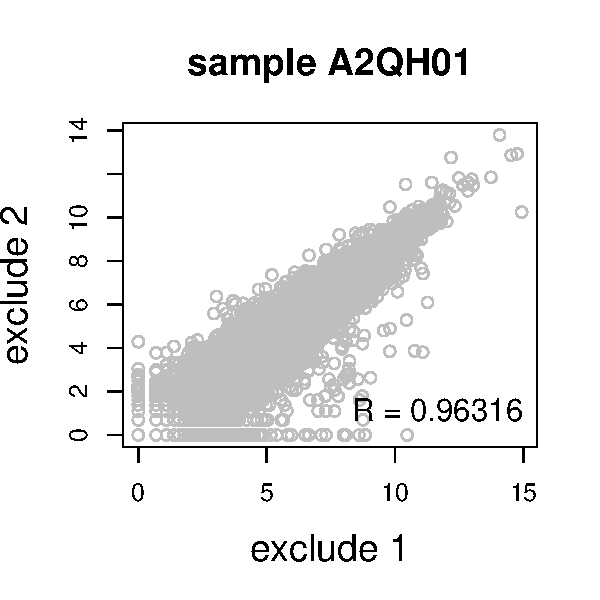
\includegraphics{Rep_picking_CutCut2.pdf}
   }
    \caption[Replicate excluded samples]{\small \textbf{Replicate excluded samples.} Both tumour samples of patient A2QH were excluded as they were poorly correlated with other samples, although they are highly similar to each other as shown by Pearson's correlation of log-raw counts.
}
\label{fig:rep_cutcut}
\end{mdframed}
\end{figure*}

\begin{figure*}[!ht]
\begin{mdframed}
           \begin{center}
%
        \subfigure[Remaining triplet]{%
           \label{fig:rep_keepcut:A26J:first}
           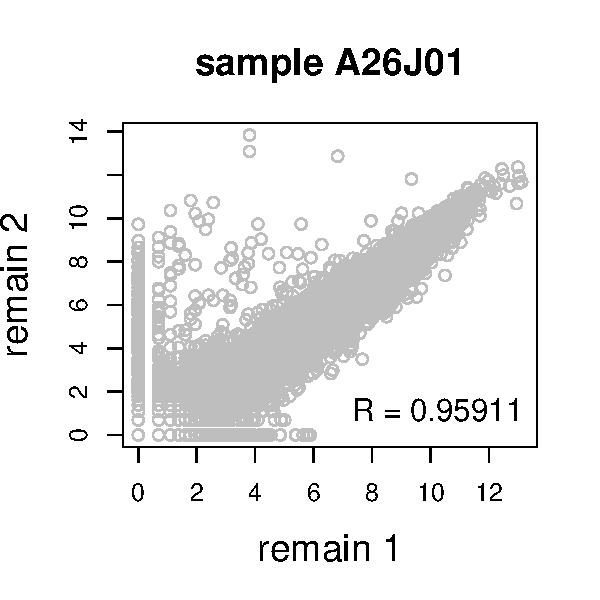
\includegraphics[width=0.3\textwidth]{Rep_picking_KeepKeep(1).pdf}}
        }%
        \subfigure[Remaining triplet]{%
           \label{fig:rep_keepcut:A26J:second}
           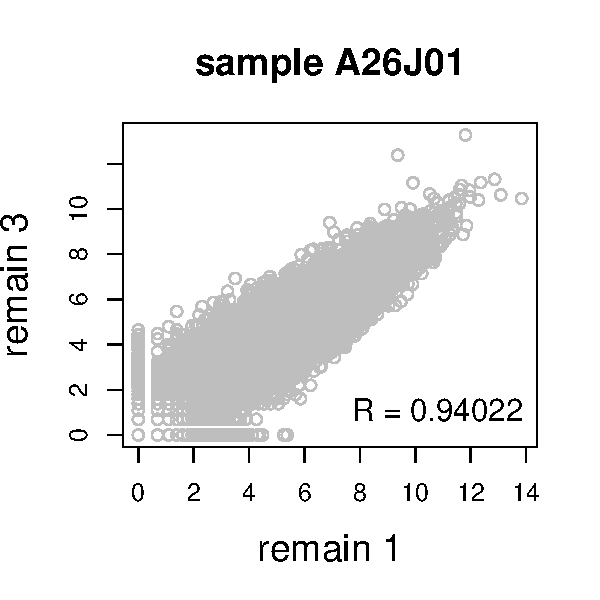
\includegraphics[width=0.3\textwidth]{Rep_picking_KeepKeep(2).pdf}}
        }%
        \subfigure[Remaining triplet]{%
           \label{fig:rep_keepcut:A26J:third}
           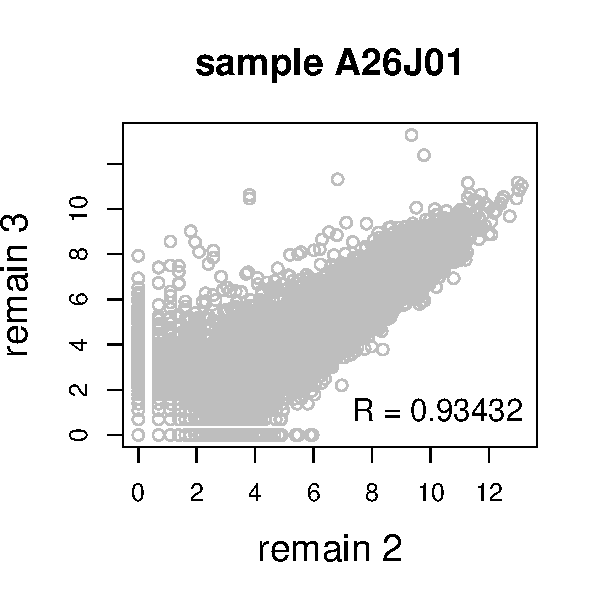
\includegraphics[width=0.3\textwidth]{Rep_picking_KeepKeep(3).pdf}}
        }%
%

%
        \subfigure[Remaining paired samples]{%
           \label{fig:rep_keepcut:A13G}
           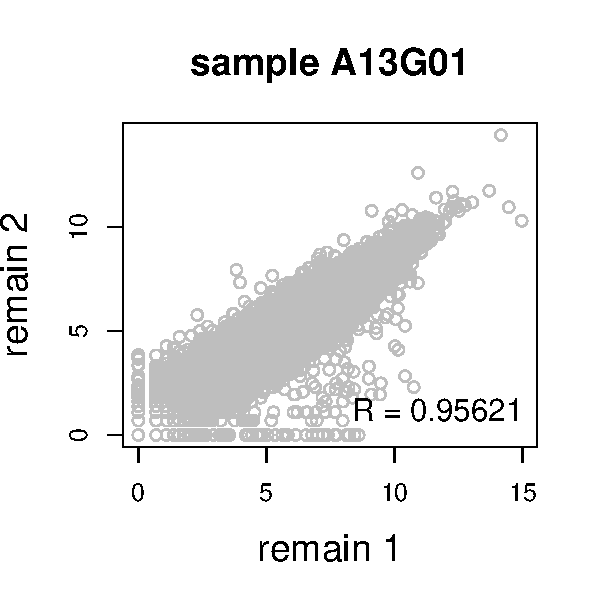
\includegraphics[width=0.3\textwidth]{Rep_picking_KeepKeep(4).pdf}}
        }%
        \subfigure[Remaining paired samples]{%
           \label{fig:rep_keepcut:A26F}
           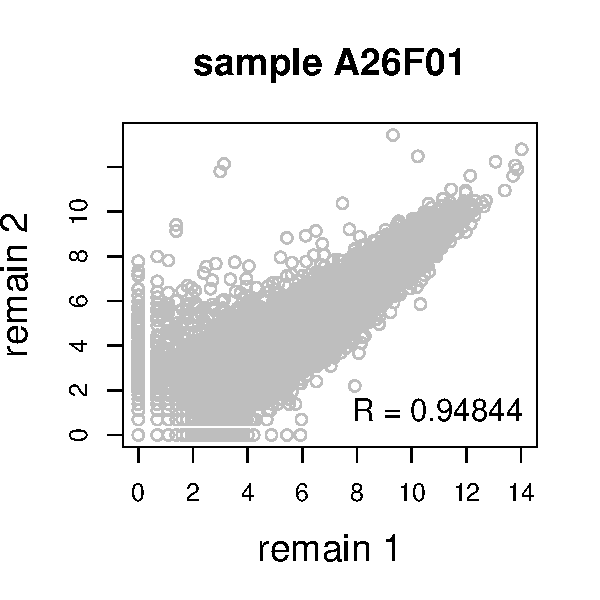
\includegraphics[width=0.3\textwidth]{Rep_picking_KeepKeep(5).pdf}}
        }%
        \subfigure[Remaining paired samples]{%
           \label{fig:rep_keepcut:A3OD}
           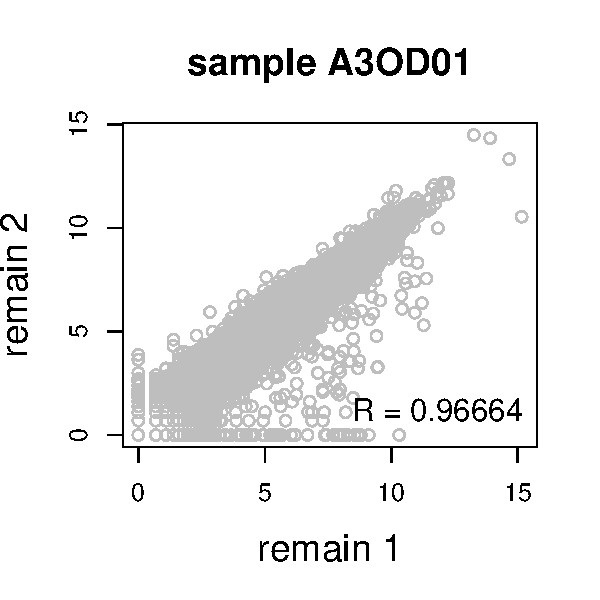
\includegraphics[width=0.3\textwidth]{Rep_picking_KeepKeep(6).pdf}}
        }%
%
    \end{center}
    \caption[Replicate samples with all remaining]{\small \textbf{Replicate samples with all remaining.} Patient A26J was sampled 3 times and compared pairwise. Pairs of samples were also compared for other patients with replicate samples.  In all cases, replicate samples remaining in the dataset were highly concordant as shown by Pearson's correlation of log-raw counts.
}
\label{fig:rep_keepkeep}
\end{mdframed}
\end{figure*}


\begin{figure*}[!ht]
\begin{mdframed}
           \begin{center}
%
        \subfigure[Remaining]{%
           \label{fig:rep_keepcut:A0DB:first}
           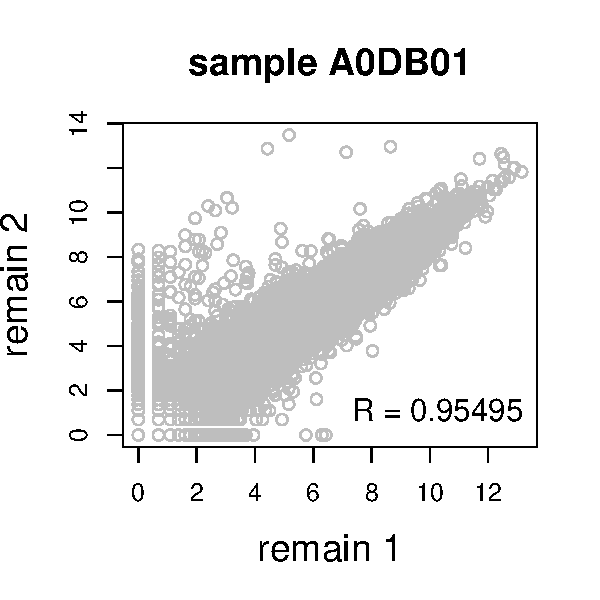
\includegraphics[width=0.3\textwidth]{Rep_picking_KeepCut(1).pdf}}
        }%
        \subfigure[Compare with excluded]{%
           \label{fig:rep_keepcut:A0DB:second}
           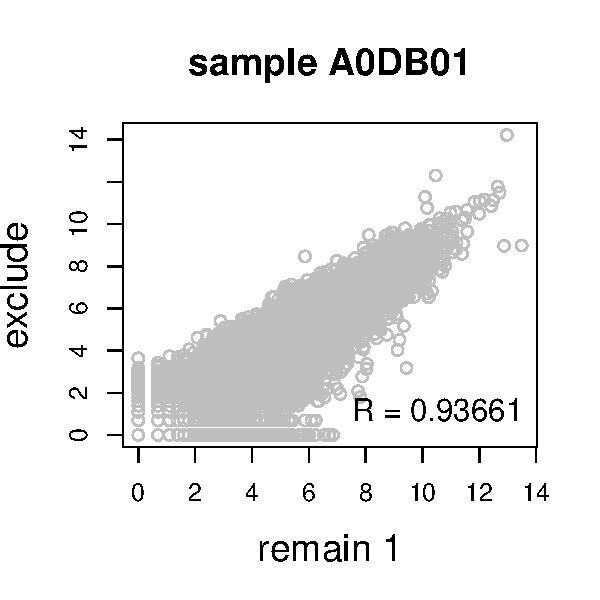
\includegraphics[width=0.3\textwidth]{Rep_picking_KeepCut(2).pdf}}
        }%
        \subfigure[Compare with excluded]{%
           \label{fig:rep_keepcut:A0DB:third}
           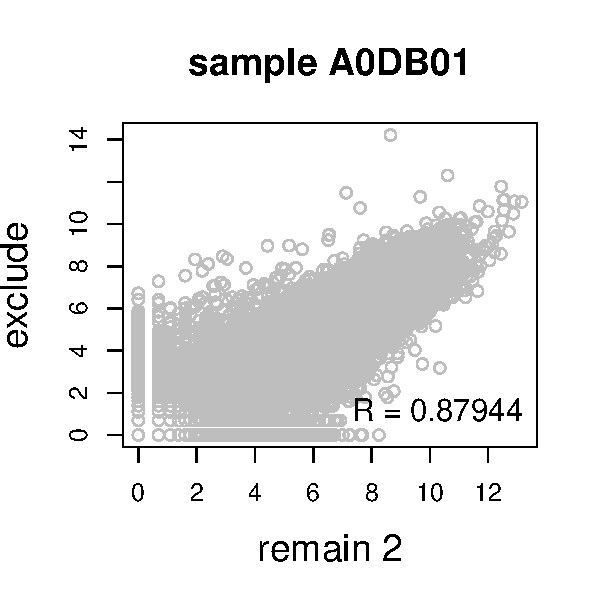
\includegraphics[width=0.3\textwidth]{Rep_picking_KeepCut(3).pdf}}
        }%
%

%
        \subfigure[Remaining]{%
           \label{fig:rep_keepcut:A13D:first}
           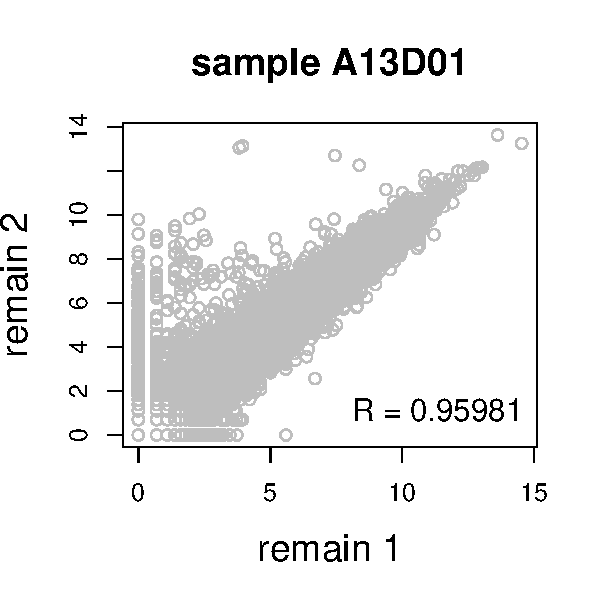
\includegraphics[width=0.3\textwidth]{Rep_picking_KeepCut(4).pdf}}
        }%
        \subfigure[Compare with excluded]{%
           \label{fig:rep_keepcut:A13D:second}
           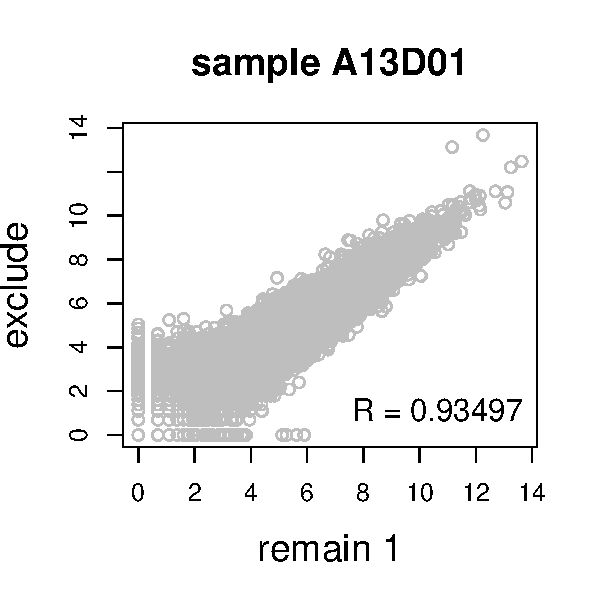
\includegraphics[width=0.3\textwidth]{Rep_picking_KeepCut(5).pdf}}
        }%
        \subfigure[Compare with excluded]{%
           \label{fig:rep_keepcut:A13D:third}
           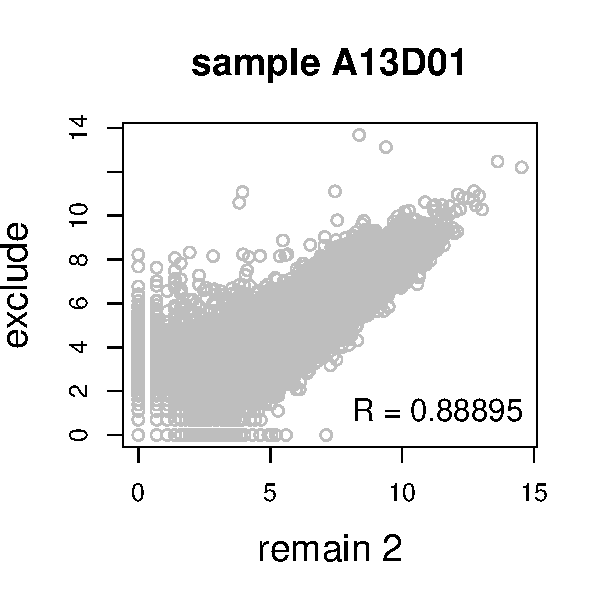
\includegraphics[width=0.3\textwidth]{Rep_picking_KeepCut(6).pdf}}
        }%
%

%
        \subfigure[Remaining]{%
           \label{fig:rep_keepcut:A13E:first}
           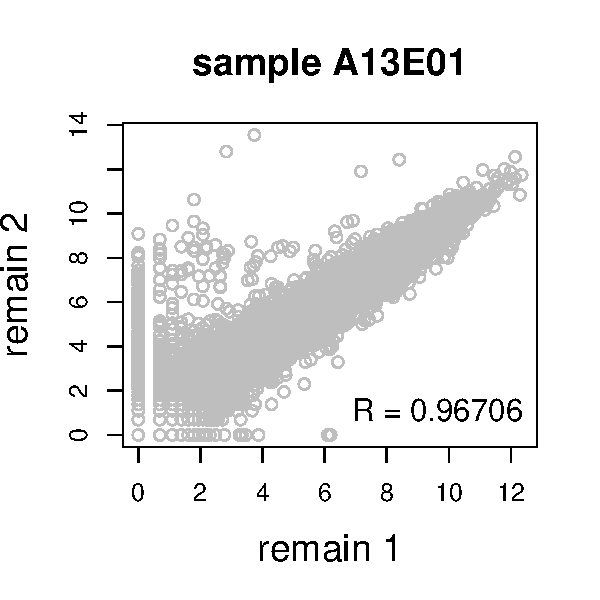
\includegraphics[width=0.3\textwidth]{Rep_picking_KeepCut(7).pdf}}
        }%
        \subfigure[Compare with excluded]{%
           \label{fig:rep_keepcut:A13E:second}
           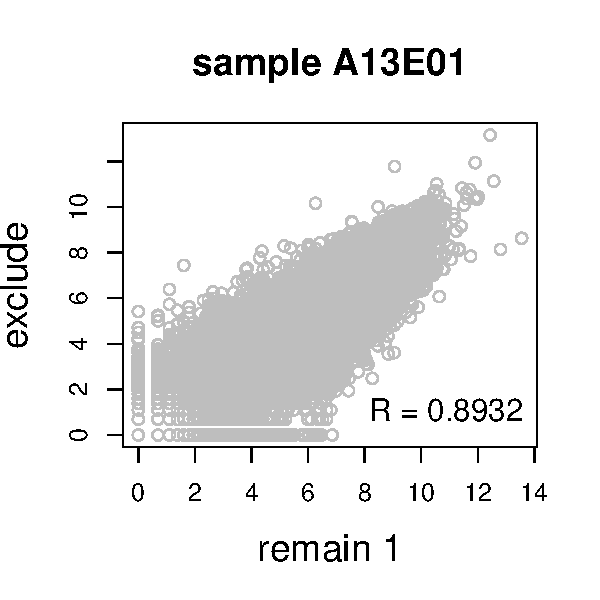
\includegraphics[width=0.3\textwidth]{Rep_picking_KeepCut(8).pdf}}
        }%
        \subfigure[Compare with excluded]{%
           \label{fig:rep_keepcut:A13E:third}
           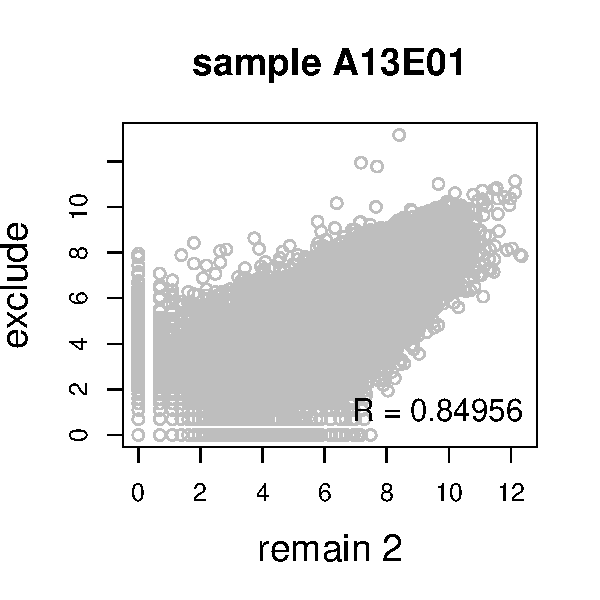
\includegraphics[width=0.3\textwidth]{Rep_picking_KeepCut(9).pdf}}
        }%
%
    \end{center}
    \caption[Replicate samples with some excluded]{\small \textbf{Replicate samples with some excluded.} Patients A0DB, A13D, A13E, and A26E were each sampled 3 times and compared pairwise. Pairs of samples were also compared for other patients with replicate samples. In all cases, the replicate samples remaining in the dataset more were highly concordant (as shown by Pearson's correlation of log-raw counts) than those excluded from the analysis.
}
\end{mdframed}
\end{figure}
\begin{figure}[!ht]\ContinuedFloat
\begin{mdframed}
     \begin{center}
%
        \subfigure[Remaining]{%
           \addtocounter{subfigure}{9}
           \label{fig:rep_keepcut:A26E:first}
           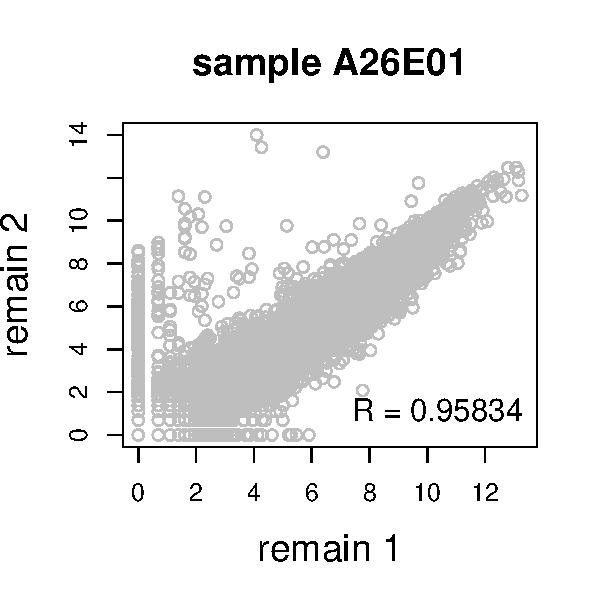
\includegraphics[width=0.3\textwidth]{Rep_picking_KeepCut(10).pdf}}
        }%
        \subfigure[Compare with excluded]{%
           \label{fig:rep_keepcut:A26E:second}
           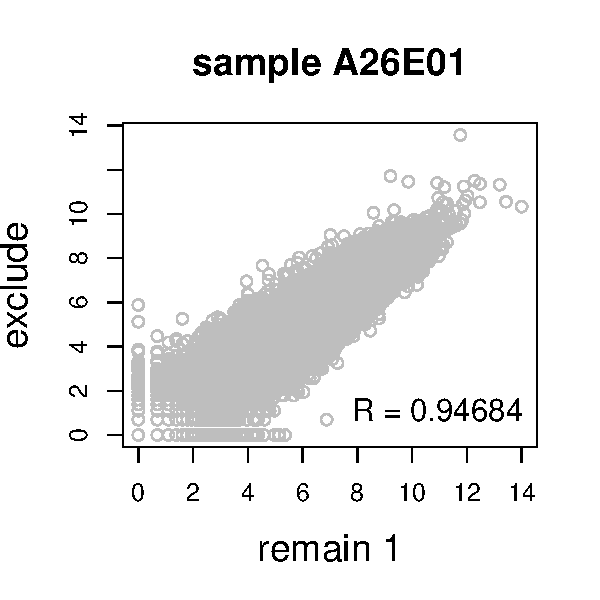
\includegraphics[width=0.3\textwidth]{Rep_picking_KeepCut(11).pdf}}
        }%
        \subfigure[Compare with excluded]{%
           \label{fig:rep_keepcut:A26E:third}
           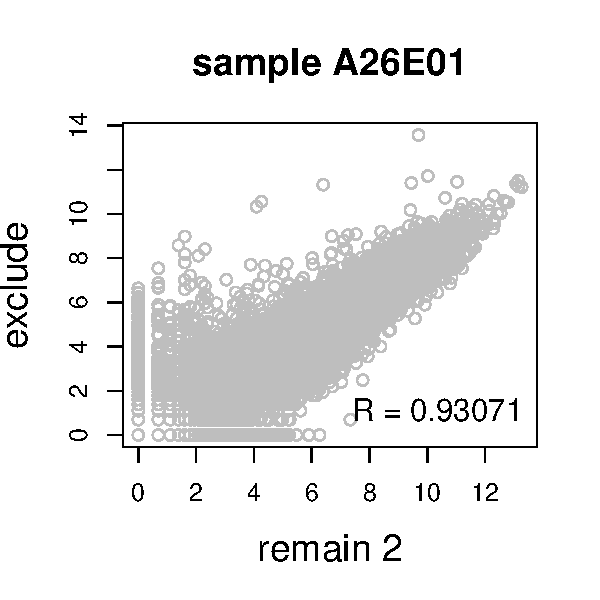
\includegraphics[width=0.3\textwidth]{Rep_picking_KeepCut(12).pdf}}
        }%
%

%
        \subfigure[Compare with excluded]{%
           \label{fig:rep_keepcut:A0DC}
           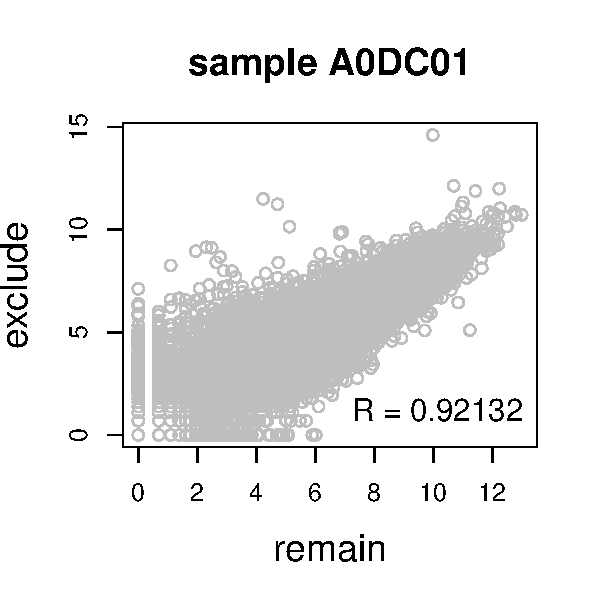
\includegraphics[width=0.3\textwidth]{Rep_picking_KeepCut(13).pdf}}
        }%
        \subfigure[Compare with excluded]{%
           \label{fig:rep_keepcut:A26I}
           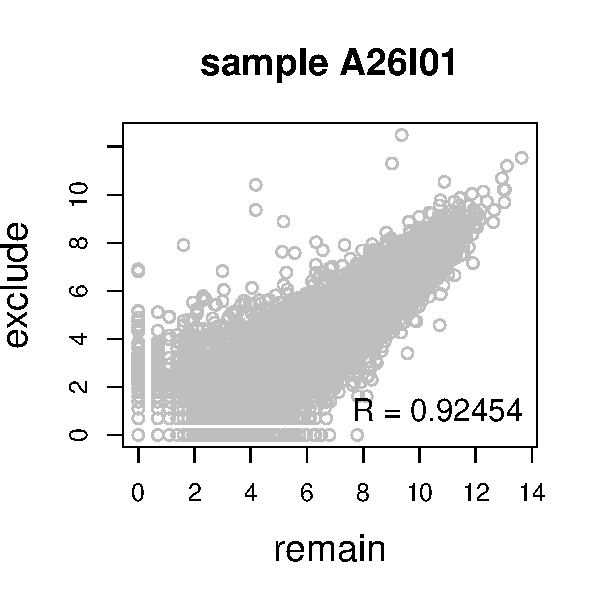
\includegraphics[width=0.3\textwidth]{Rep_picking_KeepCut(14).pdf}}
        }%
%
    \end{center}
    \caption[Replicate samples with some excluded]{\small \textbf{Replicate samples with some excluded.} Patients A0DB, A13D, A13E, and A26E were each sampled 3 times and compared pairwise. Pairs of samples were also compared for other patients with replicate samples. In all cases, the replicate samples remaining in the dataset more were highly concordant (as shown by Pearson's correlation of log-raw counts) than those excluded from the analysis.
}
\label{fig:rep_keepcut}
\end{mdframed}
\end{figure*}

\chapter{Mutation Analysis in Breast Cancer}
\label{appendix:mtSL}


\begin{table*}[!ht]
\caption{Candidate synthetic lethal genes against E-cadherin from mtSLIPT}
\label{tab:gene_mtSL}
\centering
\resizebox{0.8 \textwidth}{!}{
\begin{threeparttable}
\begin{tabular}{>{\em}sl^c^c^c^c^c}
\rowstyle{\bfseries}
 \em{Gene} & Observed & Expected & $\chi^2$ value & p-value & p-value (FDR) \\ 
  \hline
  \rowcolor{black!10}
TFAP2B & 8 & 36.7 & 89.5 & $3.60 \times 10^{-20}$ & $8.37 \times 10^{-17}$ \\
  \rowcolor{black!5}
  ZNF423 & 15 & 36.7 & 78.8 & $7.89 \times 10^{-18}$ & $1.22 \times 10^{-14}$ \\ 
  \rowcolor{black!10}
  CALCOCO1 & 11 & 36.7 & 76.8 & $2.09 \times 10^{-17}$ & $2.59 \times 10^{-14}$ \\ 
  \rowcolor{black!5}
  RBM5 & 13 & 36.7 & 75.7 & $3.65 \times 10^{-17}$ & $4.00 \times 10^{-14}$ \\ 
  \rowcolor{black!10}
  BTG2 & 7 & 36.7 & 71.7 & $2.72 \times 10^{-16}$ & $1.81 \times 10^{-13}$ \\ 
  \rowcolor{black!5}
  RXRA & 6 & 36.7 & 70.5 & $5.00 \times 10^{-16}$ & $2.97 \times 10^{-13}$ \\ 
  \rowcolor{black!10}
  SLC27A1 & 11 & 36.7 & 70.3 & $5.42 \times 10^{-16}$ & $2.97 \times 10^{-13}$ \\ 
  \rowcolor{black!5}
  MEF2D & 12 & 36.7 & 69.6 & $7.86 \times 10^{-16}$ & $3.95 \times 10^{-13}$ \\ 
  \rowcolor{black!10}
  NISCH & 12 & 36.7 & 69.6 & $7.86 \times 10^{-16}$ & $3.95 \times 10^{-13}$ \\ 
  \rowcolor{black!5}
  AVPR2 & 9 & 36.7 & 69.2 & $9.36 \times 10^{-16}$ & $4.58 \times 10^{-13}$ \\ 
  \rowcolor{black!10}
  CRY2 & 13 & 36.7 & 68.9 & $1.07 \times 10^{-15}$ & $4.98 \times 10^{-13}$ \\ 
  \rowcolor{black!5}
  RAPGEF3 & 13 & 36.7 & 68.9 & $1.07 \times 10^{-15}$ & $4.98 \times 10^{-13}$ \\ 
  \rowcolor{black!10}
  NRIP2 & 10 & 36.7 & 68.2 & $1.58 \times 10^{-15}$ & $7.18 \times 10^{-13}$ \\ 
  \rowcolor{black!5}
  DARC & 12 & 36.7 & 66.4 & $3.76 \times 10^{-15}$ & $1.54 \times 10^{-12}$ \\ 
  \rowcolor{black!10}
  SFRS5 & 12 & 36.7 & 66.4 & $3.76 \times 10^{-15}$ & $1.54 \times 10^{-12}$ \\ 
  \rowcolor{black!5}
  NOSTRIN & 5 & 36.7 & 65.1 & $7.40 \times 10^{-15}$ & $2.70 \times 10^{-12}$ \\ 
  \rowcolor{black!10}
  KIF13B & 12 & 36.7 & 63.4 & $1.69 \times 10^{-14}$ & $5.16 \times 10^{-12}$ \\ 
  \rowcolor{black!5}
  TENC1 & 10 & 36.7 & 62.5 & $2.67 \times 10^{-14}$ & $7.40 \times 10^{-12}$ \\ 
  \rowcolor{black!10}
  MFAP4 & 12 & 36.7 & 60.5 & $7.17 \times 10^{-14}$ & $1.67 \times 10^{-11}$ \\ 
  \rowcolor{black!5}
  ELN & 13 & 36.7 & 59.7 & $1.07 \times 10^{-13}$ & $2.32 \times 10^{-11}$ \\ 
  \rowcolor{black!10}
  SGK223 & 14 & 36.7 & 59 & $1.51 \times 10^{-13}$ & $3.05 \times 10^{-11}$ \\ 
  \rowcolor{black!5}
  KIF12 & 11 & 36.7 & 58.8 & $1.74 \times 10^{-13}$ & $3.34 \times 10^{-11}$ \\ 
  \rowcolor{black!10}
  SELP & 11 & 36.7 & 58.8 & $1.74 \times 10^{-13}$ & $3.34 \times 10^{-11}$ \\ 
  \rowcolor{black!5}
  CIRBP & 9 & 36.7 & 58.7 & $1.83 \times 10^{-13}$ & $3.41 \times 10^{-11}$ \\ 
  \rowcolor{black!10}
  CTDSP1 & 9 & 36.7 & 58.7 & $1.83 \times 10^{-13}$ & $3.41 \times 10^{-11}$ \\
   \hline
\end{tabular}
\begin{tablenotes}
\raggedright \small
Strongest candidate SL partners for \textit{CDH1} by mtSLIPT with observed and expected mutant samples with low expression of partner genes
\end{tablenotes}
\end{threeparttable}
}
\end{table*}


\begin{table*}[!ht]
\caption{Pathways for \textit{CDH1} partners from mtSLIPT}
\label{tab:pathway_mtSL}
\centering
\resizebox{1 \textwidth}{!}{
\begin{threeparttable}
\begin{tabular}{lccc}
  \hline
 \textbf{Pathways Over-represented} & \textbf{Pathway Size} & \textbf{SL Genes} & \textbf{p-value (FDR)} \\
  \hline
  \rowcolor{black!10}
  Eukaryotic Translation Elongation &  86 &  60 & $2.0 \times 10^{-128}$ \\ 
  \rowcolor{black!5}
  Peptide chain elongation &  83 &  59 & $2.0 \times 10^{-128}$ \\ 
  \rowcolor{black!10}
  Eukaryotic Translation Termination &  83 &  58 & $2.3 \times 10^{-125}$ \\ 
  \rowcolor{black!5}
  Viral mRNA Translation &  81 &  57 & $2.5 \times 10^{-124}$ \\ 
  \rowcolor{black!10}
  Nonsense Mediated Decay independent of the Exon Junction Complex &  88 &  59 & $8.6 \times 10^{-124}$ \\ 
  \rowcolor{black!5}
  Nonsense-Mediated Decay & 103 &  61 & $5.2 \times 10^{-117}$ \\ 
  \rowcolor{black!10}
  Nonsense Mediated Decay enhanced by the Exon Junction Complex & 103 &  61 & $5.2 \times 10^{-117}$ \\ 
  \rowcolor{black!5}
  Formation of a pool of free 40S subunits &  93 &  58 & $1.6 \times 10^{-116}$ \\ 
  \rowcolor{black!10}
  L13a-mediated translational silencing of Ceruloplasmin expression & 103 &  59 & $1.3 \times 10^{-111}$ \\ 
  \rowcolor{black!5}
  3' -UTR-mediated translational regulation & 103 &  59 & $1.3 \times 10^{-111}$ \\ 
  \rowcolor{black!10}
  GTP hydrolysis and joining of the 60S ribosomal subunit & 104 &  59 & $6.2 \times 10^{-111}$ \\ 
  \rowcolor{black!5}
  SRP-dependent cotranslational protein targeting to membrane & 104 &  58 & $2.9 \times 10^{-108}$ \\ 
  \rowcolor{black!10}
  Eukaryotic Translation Initiation & 111 &  59 & $3.0 \times 10^{-106}$ \\ 
  \rowcolor{black!5}
  Cap-dependent Translation Initiation & 111 &  59 & $3.0 \times 10^{-106}$ \\ 
  \rowcolor{black!10}
  Influenza Viral RNA Transcription and Replication & 108 &  57 & $5.1 \times 10^{-103}$ \\ 
  \rowcolor{black!5}
  Influenza Infection & 117 &  59 & $1.5 \times 10^{-102}$ \\ 
  \rowcolor{black!10}
  Translation & 141 &  64 & $3.7 \times 10^{-101}$ \\ 
  \rowcolor{black!5}
  Influenza Life Cycle & 112 &  57 & $1.4 \times 10^{-100}$ \\ 
  \rowcolor{black!10}
  GPCR downstream signaling & 472 & 116 & $1.0 \times 10^{-80}$ \\ 
  \rowcolor{black!5}
  Hemostasis & 422 & 105 & $1.4 \times 10^{-78}$ \\ 
  \hline
\end{tabular}
\begin{tablenotes}
\raggedright \small
Gene set over-representation analysis (hypergeometric test) for Reactome pathways in mtSLIPT partners for \textit{CDH1}
\end{tablenotes}
\end{threeparttable}
}
\end{table*}

\begin{figure*}[!ht]
\begin{mdframed}
  \centering
  \resizebox{0.99 \textwidth}{!}{
    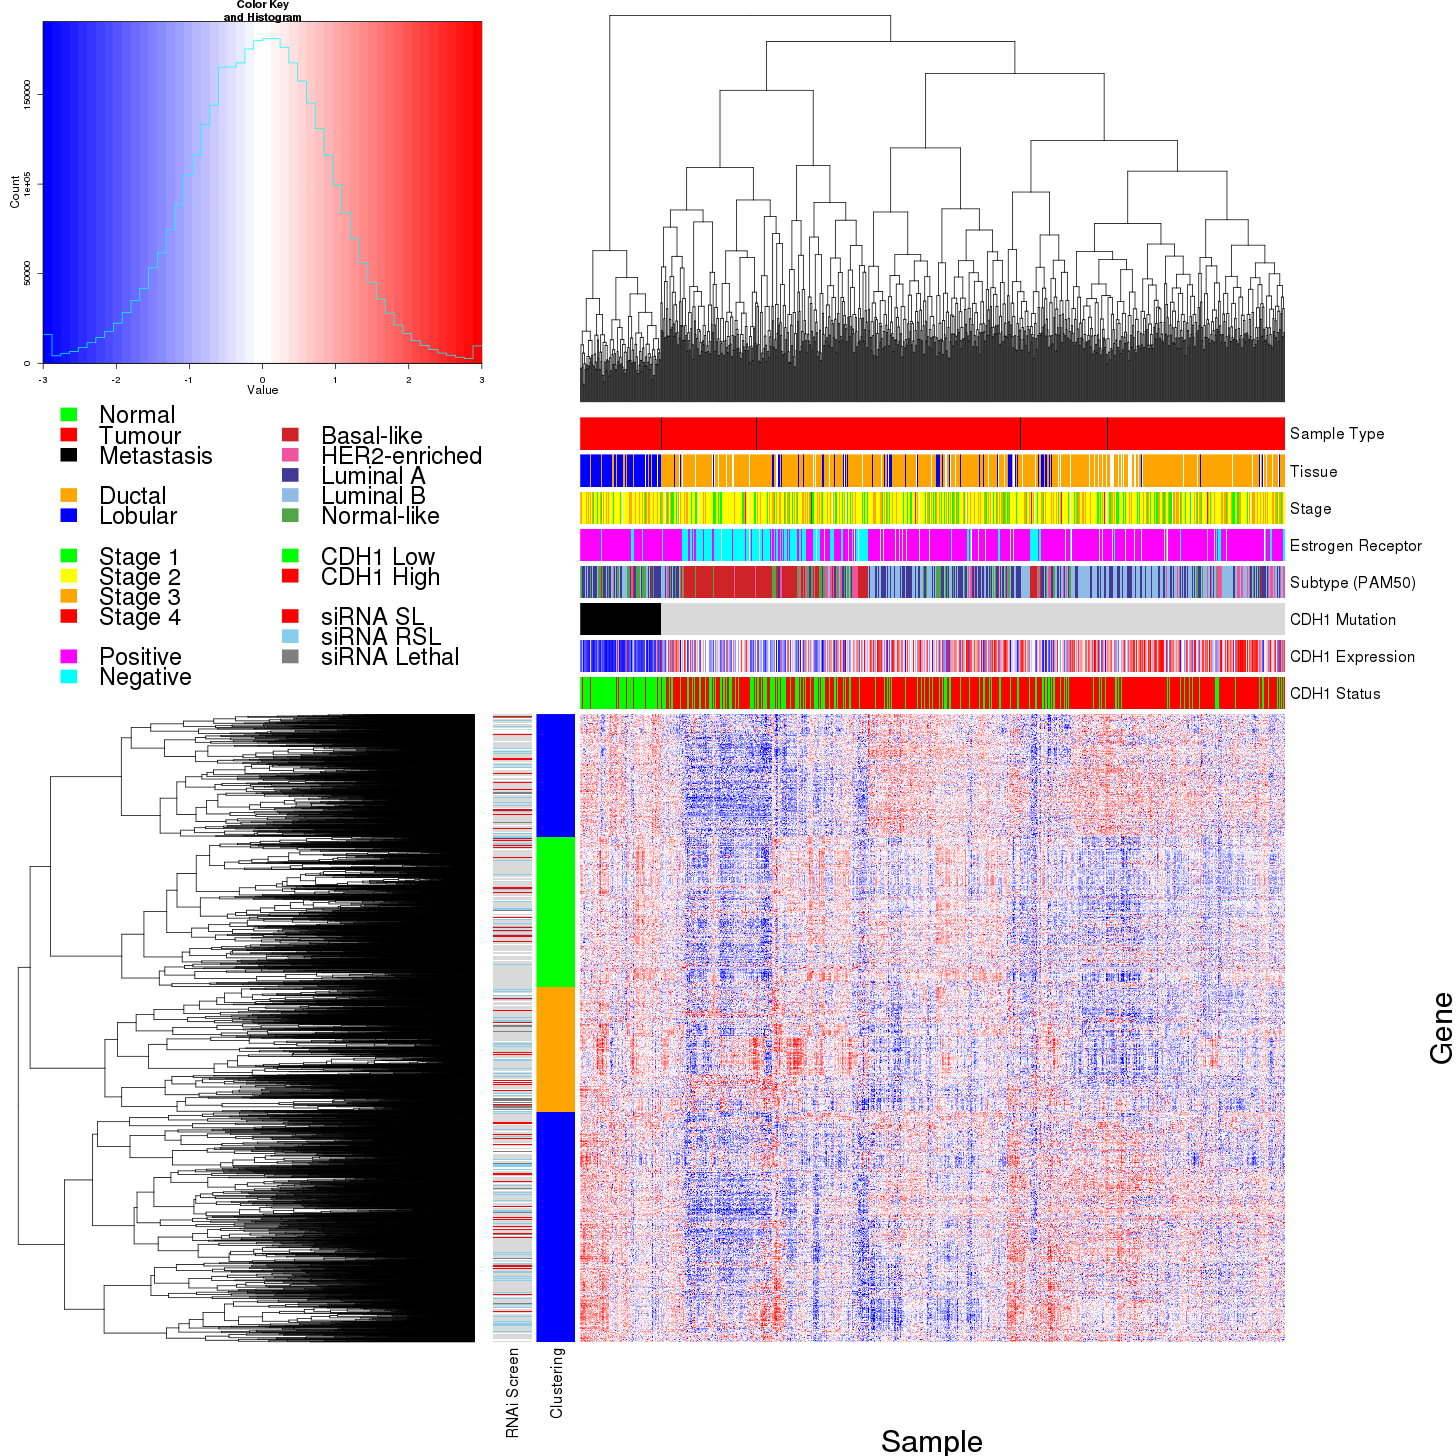
\includegraphics{CDH1_Heatmaps_Genes_Split_By_CDH1_z-trans_mtSL_cordistx_Pub.png}
   }
    \caption[Synthetic lethal expression profiles of analysed samples]{\small \textbf{Synthetic lethal expression profiles of analysed samples.} Gene expression profile heatmap (correlation distance) of all samples (separated by the $\sfrac{1}{3}$ quantile of \textit{CDH1} expression) analysed in TCGA breast cancer dataset for gene expression of 4,629 candidate partners of E-cadherin (\textit{CDH1}) from SLIPT prediction (with significant FDR adjusted $p < 0.05$). Deeply clustered, inter-correlated genes form several main groups, each containing genes that were SL candidates or toxic in an siRNA screen \cite{Telford2015}. Clusters had different sample groups highly expressing the synthetic lethal candidates in \textit{CDH1} low samples, notably 'normal-like', basal, and estrogen receptor negative samples have elevated expression in one or more distinct clusters showing complexity and variation among candidate synthetic lethal partners. \textit{CDH1} low samples also contained most of samples with \textit{CDH1} mutations.
   %This suggests that multiple targets may be needed to target \textit{CDH1} deficiency across genetic backgrounds and that combination therapy may be more effective. 
}
\label{fig:slipt_expr_mtSL}
\end{mdframed}
\end{figure*}


\begin{table*}[!Hp]
\caption{Pathway composition for clusters of \textit{CDH1} partners from mtSLIPT}
\label{tab:pathway_clusters_mtSL}
\centering
%\begin{tiny}
%\makebox[\textwidth][c]{
\resizebox{0.666 \textwidth}{!}{
\begin{tabular}{lccc}
%\caption{Pathway composition for clusters of \textit{CDH1} partners from SLIPT}
%\label{tab:pathway_clusters}
  \large{\textbf{Pathways Over-represented in Cluster 1}} & \large{\textbf{Pathway Size}} & \large{\textbf{Cluster Genes}} & \large{\textbf{p-value (FDR)}} \\ %(833 genes)  
  \hline
  \rowcolor{Cluster_Blue!20}
  Olfactory Signaling Pathway &  57 &   8 & $7.1 \times 10^{-9}$ \\ 
  \rowcolor{Cluster_Blue!15} 
  Assembly of the primary cilium & 149 &  14 & $8 \times 10^{-9}$ \\ 
  \rowcolor{Cluster_Blue!20} 
  Sphingolipid metabolism &  62 &   8 & $9.6 \times 10^{-9}$ \\ 
  \rowcolor{Cluster_Blue!15} 
  Signaling by ERBB4 & 133 &  12 & $5.1 \times 10^{-8}$ \\ 
  \rowcolor{Cluster_Blue!20} 
  PI3K Cascade &  65 &   7 & $4.9 \times 10^{-7}$ \\ 
  \rowcolor{Cluster_Blue!15} 
  Circadian Clock &  33 &   5 & $4.9 \times 10^{-7}$ \\ 
  \rowcolor{Cluster_Blue!20} 
  Nuclear signaling by ERBB4 &  34 &   5 & $4.9 \times 10^{-7}$ \\ 
  \rowcolor{Cluster_Blue!15} 
  Intraflagellar transport &  35 &   5 & $4.9 \times 10^{-7}$ \\ 
  \rowcolor{Cluster_Blue!20} 
  PI3K events in ERBB4 signaling &  87 &   8 & $4.9 \times 10^{-7}$ \\ 
  \rowcolor{Cluster_Blue!15} 
  PIP3 activates AKT signaling &  87 &   8 & $4.9 \times 10^{-7}$ \\ 
  \rowcolor{Cluster_Blue!20} 
  PI3K events in ERBB2 signaling &  87 &   8 & $4.9 \times 10^{-7}$ \\ 
  \rowcolor{Cluster_Blue!15} 
  PI-3K cascade:FGFR1 &  87 &   8 & $4.9 \times 10^{-7}$ \\ 
  \rowcolor{Cluster_Blue!20} 
  PI-3K cascade:FGFR2 &  87 &   8 & $4.9 \times 10^{-7}$ \\ 
  \rowcolor{Cluster_Blue!15} 
  PI-3K cascade:FGFR3 &  87 &   8 & $4.9 \times 10^{-7}$ \\ 
  \rowcolor{Cluster_Blue!20} 
  PI-3K cascade:FGFR4 &  87 &   8 & $4.9 \times 10^{-7}$ \\ 
  \rowcolor{Cluster_Blue!15} 
  Deadenylation of mRNA &  22 &   4 & $5.6 \times 10^{-7}$ \\ 
  \rowcolor{Cluster_Blue!20} 
  PI3K/AKT activation &  90 &   8 & $5.6 \times 10^{-7}$ \\ 
  \rowcolor{Cluster_Blue!15} 
  Cargo trafficking to the periciliary membrane &  38 &   5 & $5.6 \times 10^{-7}$ \\ 
  \rowcolor{Cluster_Blue!20} 
  Signaling by Hedgehog & 108 &   9 & $5.6 \times 10^{-7}$ \\ 
  \rowcolor{Cluster_Blue!15} 
  Downstream signal transduction & 143 &  11 & $5.6 \times 10^{-7}$ \\ 
  \hline
  \\
  \cellcolor{white} \large{\textbf{Pathways Over-represented in Cluster 2}} & \large{\textbf{Pathway Size}} & \large{\textbf{Cluster Genes}} & \large{\textbf{p-value (FDR)}} \\ %(833 genes)  
  \hline
  \rowcolor{Cluster_Green!20}
  G$_{\alpha s}$ signalling events &  83 &  19 & $5.1 \times 10^{-25}$ \\ 
  \rowcolor{Cluster_Green!15}
  Extracellular matrix organization & 238 &  30 & $1.4 \times 10^{-18}$ \\ 
  \rowcolor{Cluster_Green!20} 
  Hemostasis & 422 &  46 & $2.7 \times 10^{-16}$ \\ 
  \rowcolor{Cluster_Green!15} 
  Aquaporin-mediated transport &  32 &   9 & $2.7 \times 10^{-16}$ \\ 
  \rowcolor{Cluster_Green!20} 
  Transcriptional regulation of white adipocyte differentiation &  56 &  11 & $1.7 \times 10^{-15}$ \\ 
  \rowcolor{Cluster_Green!15} 
  Degradation of the extracellular matrix & 102 &  15 & $1.7 \times 10^{-15}$ \\ 
  \rowcolor{Cluster_Green!20} 
  Integration of energy metabolism &  84 &  13 & $8.8 \times 10^{-15}$ \\ 
  \rowcolor{Cluster_Green!15} 
  GPCR downstream signaling & 472 &  48 & $2.8 \times 10^{-14}$ \\ 
  \rowcolor{Cluster_Green!20} 
  G$_{\alpha z}$ signalling events &  15 &   6 & $5 \times 10^{-14}$ \\ 
  \rowcolor{Cluster_Green!15} 
  Molecules associated with elastic fibres &  33 &   8 & $5.4 \times 10^{-14}$ \\ 
  \rowcolor{Cluster_Green!20} 
  Phase 1 - Functionalization of compounds &  67 &  11 & $5.6 \times 10^{-14}$ \\ 
  \rowcolor{Cluster_Green!15} 
  Platelet activation, signaling and aggregation & 179 &  20 & $5.6 \times 10^{-14}$ \\ 
  \rowcolor{Cluster_Green!20} 
  Vasopressin regulates renal water homeostasis via Aquaporins &  24 &   7 & $6.1 \times 10^{-14}$ \\ 
  \rowcolor{Cluster_Green!15} 
  Elastic fibre formation &  37 &   8 & $3 \times 10^{-13}$ \\ 
  \rowcolor{Cluster_Green!20} 
  Calmodulin induced events &  27 &   7 & $3.3 \times 10^{-13}$ \\ 
  \rowcolor{Cluster_Green!15} 
  CaM pathway &  27 &   7 & $3.3 \times 10^{-13}$ \\ 
  \rowcolor{Cluster_Green!20} 
  cGMP effects &  18 &   6 & $3.6 \times 10^{-13}$ \\ 
  \rowcolor{Cluster_Green!15} 
  G$_{\alpha i}$ signalling events & 167 &  18 & $6.3 \times 10^{-13}$ \\ 
  \rowcolor{Cluster_Green!20} 
  Ca-dependent events &  29 &   7 & $8.2 \times 10^{-13}$ \\ 
  \rowcolor{Cluster_Green!15} 
  Binding and Uptake of Ligands by Scavenger Receptors &  40 &   8 & $8.2 \times 10^{-13}$ \\ 
  \hline
  \\
  \cellcolor{white} \large{\textbf{Pathways Over-represented in Cluster 3}} & \large{\textbf{Pathway Size}} & \large{\textbf{Cluster Genes}} & \large{\textbf{p-value (FDR)}} \\ %(833 genes)  
  \hline
  \rowcolor{Cluster_Orange!30}
  Eukaryotic Translation Elongation &  86 &  55 & $1.1 \times 10^{-112}$ \\ 
  \rowcolor{Cluster_Orange!20} 
  Peptide chain elongation &  83 &  54 & $1.3 \times 10^{-112}$ \\ 
  \rowcolor{Cluster_Orange!30} 
  Viral mRNA Translation &  81 &  53 & $1.6 \times 10^{-111}$ \\ 
  \rowcolor{Cluster_Orange!20} 
  Eukaryotic Translation Termination &  83 &  53 & $7.1 \times 10^{-110}$ \\ 
  \rowcolor{Cluster_Orange!30} 
  Nonsense Mediated Decay independent of the Exon Junction Complex &  88 &  54 & $1 \times 10^{-108}$ \\ 
  \rowcolor{Cluster_Orange!20} 
  Formation of a pool of free 40S subunits &  93 &  53 & $4.1 \times 10^{-102}$ \\ 
  \rowcolor{Cluster_Orange!30} 
  Nonsense-Mediated Decay & 103 &  54 & $3.9 \times 10^{-98}$ \\ 
  \rowcolor{Cluster_Orange!20} 
  Nonsense Mediated Decay enhanced by the Exon Junction Complex & 103 &  54 & $3.9 \times 10^{-98}$ \\ 
  \rowcolor{Cluster_Orange!30} 
  L13a-mediated translational silencing of Ceruloplasmin expression & 103 &  53 & $1.2 \times 10^{-95}$ \\ 
  \rowcolor{Cluster_Orange!20} 
  3' -UTR-mediated translational regulation & 103 &  53 & $1.2 \times 10^{-95}$ \\ 
  \rowcolor{Cluster_Orange!30} 
  SRP-dependent cotranslational protein targeting to membrane & 104 &  53 & $4.3 \times 10^{-95}$ \\ 
  \rowcolor{Cluster_Orange!20} 
  GTP hydrolysis and joining of the 60S ribosomal subunit & 104 &  53 & $4.3 \times 10^{-95}$ \\ 
  \rowcolor{Cluster_Orange!30} 
  Influenza Viral RNA Transcription and Replication & 108 &  53 & $9.6 \times 10^{-93}$ \\ 
  \rowcolor{Cluster_Orange!20} 
  Eukaryotic Translation Initiation & 111 &  53 & $4.2 \times 10^{-91}$ \\ 
  \rowcolor{Cluster_Orange!30} 
  Cap-dependent Translation Initiation & 111 &  53 & $4.2 \times 10^{-91}$ \\ 
  \rowcolor{Cluster_Orange!20} 
  Influenza Life Cycle & 112 &  53 & $1.4 \times 10^{-90}$ \\ 
  \rowcolor{Cluster_Orange!30} 
  Influenza Infection & 117 &  53 & $6.2 \times 10^{-88}$ \\ 
  \rowcolor{Cluster_Orange!20} 
  Translation & 141 &  55 & $3 \times 10^{-81}$ \\ 
  \rowcolor{Cluster_Orange!30} 
  Formation of the ternary complex, and subsequently, the 43S complex &  47 &  23 & $2.3 \times 10^{-48}$ \\ 
  \rowcolor{Cluster_Orange!20} 
  Translation initiation complex formation &  54 &  23 & $9.1 \times 10^{-45}$ \\ 
  \hline
  \\ 
  \cellcolor{white} \large{\textbf{Pathways Over-represented in Cluster 4}} & \large{\textbf{Pathway Size}} & \large{\textbf{Cluster Genes}} & \large{\textbf{p-value (FDR)}} \\ %(833 genes)  
  \hline 
  \rowcolor{Cluster_Red!20}
  ECM proteoglycans &  66 &  10 & $2.9 \times 10^{-11}$ \\ 
  \rowcolor{Cluster_Red!15} 
  deactivation of the beta-catenin transactivating complex &  38 &   7 & $5.1 \times 10^{-10}$ \\ 
  \rowcolor{Cluster_Red!20} 
  Arachidonic acid metabolism &  41 &   7 & $1.1 \times 10^{-9}$ \\ 
  \rowcolor{Cluster_Red!15} 
  G_${\alpha q}$ signalling events & 149 &  14 & $4 \times 10^{-9}$ \\ 
  \rowcolor{Cluster_Red!20} 
  HS-GAG degradation &  21 &   5 & $4.5 \times 10^{-9}$ \\ 
  \rowcolor{Cluster_Red!15} 
  Uptake and actions of bacterial toxins &  22 &   5 & $6.1 \times 10^{-9}$ \\ 
  \rowcolor{Cluster_Red!20} 
  Gastrin-CREB signalling pathway via PKC and MAPK & 170 &  15 & $6.1 \times 10^{-9}$ \\ 
  \rowcolor{Cluster_Red!15} 
  RNA Polymerase I, RNA Polymerase III, and Mitochondrial Transcription \textcolor{Cluster_Red!15}{ll}  &  64 &   8 & $6.1 \times 10^{-9}$ \\ 
  \rowcolor{Cluster_Red!20} 
  Non-integrin membrane-ECM interactions &  53 &   7 & $1.5 \times 10^{-8}$ \\ 
  \rowcolor{Cluster_Red!15} 
  Syndecan interactions &  25 &   5 & $1.5 \times 10^{-8}$ \\ 
  \rowcolor{Cluster_Red!20} 
  NOTCH1 Intracellular Domain Regulates Transcription &  40 &   6 & $2.3 \times 10^{-8}$ \\ 
  \rowcolor{Cluster_Red!15} 
  Synthesis of Leukotrienes and Eoxins &  15 &   4 & $3.2 \times 10^{-8}$ \\ 
  \rowcolor{Cluster_Red!20} 
  Signaling by NOTCH1 &  59 &   7 & $5.3 \times 10^{-8}$ \\ 
  \rowcolor{Cluster_Red!15} 
  Regulation of insulin secretion &  44 &   6 & $6 \times 10^{-8}$ \\ 
  \rowcolor{Cluster_Red!20} 
  Metabolism of lipids and lipoproteins & 471 &  37 & $8.2 \times 10^{-8}$ \\ 
  \rowcolor{Cluster_Red!15} 
  Signaling by NOTCH &  80 &   8 & $1.2 \times 10^{-7}$ \\ 
  \rowcolor{Cluster_Red!20} 
  Platelet activation, signaling and aggregation & 179 &  14 & $1.2 \times 10^{-7}$ \\ 
  \rowcolor{Cluster_Red!15} 
  Recruitment of mitotic centrosome proteins and complexes &  64 &   7 & $1.2 \times 10^{-7}$ \\ 
  \rowcolor{Cluster_Red!20} 
  Centrosome maturation &  64 &   7 & $1.2 \times 10^{-7}$ \\ 
  \rowcolor{Cluster_Red!15} 
  Biological oxidations & 133 &  11 & $1.5 \times 10^{-7}$ \\ 
  \hline
\end{tabular}
}
\end{table*}

\begin{figure}[!ht]
\begin{mdframed}
  \centering
  \resizebox{0.66 \columnwidth}{!}{
    \includegraphics{Venn_mtSL_siRNA_allgenes_reduced_Pub.png}
   }
    \caption[Comparison of mtSLIPT to siRNA]{\small \textbf{Comparison of mtSLIPT to siRNA.} Testing the overlap of gene candidates for E-cadherin synthetic lethal partners between computational (SLIPT) and experimental screening (siRNA) approaches. The $\chi^2$ test suggests that the overlap is no more than would be expected by chance ($p = 0.281$). %A Venn diagram of all 16298 genes tested by both approaches.
}
\label{fig:Venn_allgenes_mtSL}
\end{mdframed}
\end{figure}


\begin{table*}[!Hp]
\caption{Pathway composition for \textit{CDH1} partners from mtSLIPT and siRNA}
\label{tab:Venn_over-representation_mtSL}
\centering
\resizebox{0.8 \textwidth}{!}{
\begin{tabular}{sl^c^c^c}
\rowstyle{\bfseries}
  Predicted only by SLIPT (2901 genes) & Pathway Size & Genes Identified & p-value (FDR) \\ 
  \hline
  \rowcolor{Cluster_Red!20}
  Eukaryotic Translation Elongation &  87 &  57 & $2.8 \times 10^{-120}$ \\ 
  \rowcolor{Cluster_Red!15}
  Peptide chain elongation &  84 &  56 & $3.1 \times 10^{-120}$ \\ 
  \rowcolor{Cluster_Red!20}
  Eukaryotic Translation Termination &  84 &  55 & $2.8 \times 10^{-117}$ \\ 
  \rowcolor{Cluster_Red!15}
  Viral mRNA Translation &  82 &  54 & $4.1 \times 10^{-116}$ \\ 
  \rowcolor{Cluster_Red!20}
  Nonsense Mediated Decay independent of the Exon Junction Complex &  89 &  55 & $3.7 \times 10^{-113}$ \\ 
  \rowcolor{Cluster_Red!15}
  Formation of a pool of free 40S subunits &  94 &  55 & $2.8 \times 10^{-109}$ \\ 
  \rowcolor{Cluster_Red!20}
  Nonsense-Mediated Decay & 104 &  57 & $8.4 \times 10^{-108}$ \\ 
  \rowcolor{Cluster_Red!15}
  Nonsense Mediated Decay enhanced by the Exon Junction Complex & 104 &  57 & $8.4 \times 10^{-108}$ \\ 
  \rowcolor{Cluster_Red!20}
  L13a-mediated translational silencing of Ceruloplasmin expression & 104 &  56 & $3.4 \times 10^{-105}$ \\ 
  \rowcolor{Cluster_Red!15}
  3' -UTR-mediated translational regulation & 104 &  56 & $3.4 \times 10^{-105}$ \\ 
  \rowcolor{Cluster_Red!20}
  GTP hydrolysis and joining of the 60S ribosomal subunit & 105 &  56 & $1.4 \times 10^{-104}$ \\ 
  \rowcolor{Cluster_Red!15}
  Eukaryotic Translation Initiation & 112 &  56 & $2.8 \times 10^{-100}$ \\ 
  \rowcolor{Cluster_Red!20}
  Cap-dependent Translation Initiation & 112 &  56 & $2.8 \times 10^{-100}$ \\ 
  \rowcolor{Cluster_Red!15}
  SRP-dependent cotranslational protein targeting to membrane & 105 &  54 & $2.2 \times 10^{-99}$ \\ 
  \rowcolor{Cluster_Red!20}
  Influenza Viral RNA Transcription and Replication & 109 &  54 & $5.3 \times 10^{-97}$ \\ 
  \rowcolor{Cluster_Red!15}
  Influenza Life Cycle & 113 &  54 & $9.6 \times 10^{-95}$ \\ 
  \rowcolor{Cluster_Red!20}
  Influenza Infection & 118 &  55 & $1.7 \times 10^{-94}$ \\ 
  \rowcolor{Cluster_Red!15}
  Translation & 142 &  60 & $3.5 \times 10^{-94}$ \\ 
  \rowcolor{Cluster_Red!20}
  Infectious disease & 349 &  77 & $5.9 \times 10^{-62}$ \\ 
  \rowcolor{Cluster_Red!15}
  Extracellular matrix organization & 241 &  54 & $3.0 \times 10^{-52}$ \\
  \hline
  \\
  \rowstyle{\bfseries}
  Detected only by siRNA screen (1752 genes) & Pathway Size & Genes Identified & p-value (FDR) \\ 
  \hline
  \rowcolor{Cluster_Blue!20}
  Class A/1 (Rhodopsin-like receptors) & 282 &  69 & $1.9 \times 10^{-59}$ \\ 
  \rowcolor{Cluster_Blue!15}
  GPCR ligand binding & 363 &  78 & $2.7 \times 10^{-54}$ \\ 
  \rowcolor{Cluster_Blue!20}
  Peptide ligand-binding receptors & 175 &  41 & $1.5 \times 10^{-42}$ \\ 
  \rowcolor{Cluster_Blue!15}
  $G_{\alpha i}$ signalling events & 184 &  41 & $1.1 \times 10^{-40}$ \\ 
  \rowcolor{Cluster_Blue!20}
  Gastrin-CREB signalling pathway via PKC and MAPK & 180 &  37 & $1.5 \times 10^{-35}$ \\ 
  \rowcolor{Cluster_Blue!15}
  $G_{\alpha q}$ signalling events & 159 &  34 & $3.7 \times 10^{-35}$ \\ 
  \rowcolor{Cluster_Blue!20}
  DAP12 interactions & 159 &  27 & $1.1 \times 10^{-24}$ \\ 
  \rowcolor{Cluster_Blue!15}
  VEGFA-VEGFR2 Pathway &  91 &  19 & $1.0 \times 10^{-23}$ \\ 
  \rowcolor{Cluster_Blue!20}
  Downstream signal transduction & 146 &  24 & $1.9 \times 10^{-22}$ \\ 
  \rowcolor{Cluster_Blue!15}
  Signaling by VEGF &  99 &  19 & $2.6 \times 10^{-22}$ \\ 
  \rowcolor{Cluster_Blue!20}
  DAP12 signaling & 149 &  24 & $4.2 \times 10^{-22}$ \\ 
  \rowcolor{Cluster_Blue!15}
  Organelle biogenesis and maintenance & 264 &  34 & $4.3 \times 10^{-20}$ \\ 
  \rowcolor{Cluster_Blue!20}
  Downstream signaling of activated FGFR1 & 134 &  21 & $4.3 \times 10^{-20}$ \\ 
  \rowcolor{Cluster_Blue!15}
  Downstream signaling of activated FGFR2 & 134 &  21 & $4.3 \times 10^{-20}$ \\ 
  \rowcolor{Cluster_Blue!20}
  Downstream signaling of activated FGFR3 & 134 &  21 & $4.3 \times 10^{-20}$ \\ 
  \rowcolor{Cluster_Blue!15}
  Downstream signaling of activated FGFR4 & 134 &  21 & $4.3 \times 10^{-20}$ \\ 
  \rowcolor{Cluster_Blue!20}
  Signaling by ERBB2 & 146 &  22 & $5.3 \times 10^{-20}$ \\ 
  \rowcolor{Cluster_Blue!15}
  Signaling by FGFR & 146 &  22 & $5.3 \times 10^{-20}$ \\ 
  \rowcolor{Cluster_Blue!20}
  Signaling by FGFR1 & 146 &  22 & $5.3 \times 10^{-20}$ \\ 
  \rowcolor{Cluster_Blue!15}
  Signaling by FGFR2 & 146 &  22 & $5.3 \times 10^{-20}$ \\ 
  \hline
  \\
  \rowstyle{\bfseries}
  Intersection of SLIPT and siRNA screen (450 genes) & Pathway Size & Genes Identified & p-value (FDR) \\ 
  \hline
  \rowcolor{Cluster_Red!20!Cluster_Blue!20}
  HS-GAG degradation &  21 &   4 & $4.9 \times 10^{-6}$ \\ 
  \rowcolor{Cluster_Red!15!Cluster_Blue!15}
  Retinoid metabolism and transport &  39 &   5 & $4.9 \times 10^{-6}$ \\ 
  \rowcolor{Cluster_Red!20!Cluster_Blue!20}
  Platelet activation, signaling and aggregation & 186 &  13 & $4.9 \times 10^{-6}$ \\ 
  \rowcolor{Cluster_Red!15!Cluster_Blue!15}
  Signaling by NOTCH4 &  11 &   3 & $4.9 \times 10^{-6}$ \\ 
  \rowcolor{Cluster_Red!20!Cluster_Blue!20}
  $G_{\alpha s}$ signalling events & 100 &   8 & $5.0 \times 10^{-6}$ \\ 
  \rowcolor{Cluster_Red!15!Cluster_Blue!15}
  Defective EXT2 causes exostoses 2 &  12 &   3 & $5.0 \times 10^{-6}$ \\ 
  \rowcolor{Cluster_Red!20!Cluster_Blue!20}
  Defective EXT1 causes exostoses 1, TRPS2 and CHDS &  12 &   3 & $5.0 \times 10^{-6}$ \\ 
  \rowcolor{Cluster_Red!15!Cluster_Blue!15}
  Class A/1 (Rhodopsin-like receptors) & 289 &  18 & $2.2 \times 10^{-5}$ \\ 
  \rowcolor{Cluster_Red!20!Cluster_Blue!20}
  Signaling by PDGF & 173 &  11 & $2.9 \times 10^{-5}$ \\ 
  \rowcolor{Cluster_Red!15!Cluster_Blue!15}
  Circadian Clock &  34 &   4 & $2.9 \times 10^{-5}$ \\ 
  \rowcolor{Cluster_Red!20!Cluster_Blue!20}
  Signaling by ERBB4 & 139 &   9 & $4.3 \times 10^{-5}$ \\ 
  \rowcolor{Cluster_Red!15!Cluster_Blue!15}
  Role of LAT2/NTAL/LAB on calcium mobilization &  99 &   7 & $4.4 \times 10^{-5}$ \\ 
  \rowcolor{Cluster_Red!20!Cluster_Blue!20}
  Peptide ligand-binding receptors & 181 &  11 & $4.5 \times 10^{-5}$ \\ 
  \rowcolor{Cluster_Red!15!Cluster_Blue!15}
  Defective B4GALT7 causes EDS, progeroid type &  19 &   3 & $4.5 \times 10^{-5}$ \\ 
  \rowcolor{Cluster_Red!20!Cluster_Blue!20}
  Defective B3GAT3 causes JDSSDHD &  19 &   3 & $4.5 \times 10^{-5}$ \\ 
  \rowcolor{Cluster_Red!15!Cluster_Blue!15}
  Signaling by NOTCH &  80 &   6 & $4.5 \times 10^{-5}$ \\ 
  \rowcolor{Cluster_Red!20!Cluster_Blue!20}
  $G_{\alpha q}$ signalling events & 164 &  10 & $5.1 \times 10^{-5}$ \\ 
  \rowcolor{Cluster_Red!15!Cluster_Blue!15}
  Response to elevated platelet cytosolic Ca$^{2+}$ &  84 &   6 & $7.1 \times 10^{-5}$ \\ 
  \rowcolor{Cluster_Red!20!Cluster_Blue!20}
  Signaling by ERBB2 & 148 &   9 & $7.1 \times 10^{-5}$ \\ 
  \rowcolor{Cluster_Red!15!Cluster_Blue!15}
  Signaling by SCF-KIT & 129 &   8 & $8.3 \times 10^{-5}$ \\ 
  \hline
\end{tabular}
}
\end{table*}


\begin{table*}[!Htp]
\caption{Pathways for \textit{CDH1} partners from mtSLIPT}
\label{tab:pathway_perm_mtSL}
\centering
\resizebox{0.8 \textwidth}{!}{
\begin{threeparttable}
\begin{tabular}{sl^c^c}
\rowstyle{\bfseries}
 Reactome Pathway & Over-representation & Permutation \\ 
  \hline
  \rowcolor{Cluster_Red!20} 
  \textbf{Eukaryotic Translation Elongation} & $3.2 \times 10^{-128}$ & $<7.035 \times 10^{-4}$ \\ 
    \rowcolor{Cluster_Red!15} 
  \textbf{Peptide chain elongation} & $3.2 \times 10^{-128}$ & $<7.035 \times 10^{-4}$ \\ 
    \rowcolor{Cluster_Red!20} 
  \textbf{Eukaryotic Translation Termination} & $3.7 \times 10^{-125}$ & $<7.035 \times 10^{-4}$ \\ 
    \rowcolor{Cluster_Red!15} 
  \textbf{Viral mRNA Translation} & $4.1 \times 10^{-124}$ & $<7.035 \times 10^{-4}$ \\ 
    \rowcolor{Cluster_Red!20} 
  \textbf{Nonsense Mediated Decay independent of the Exon Junction Complex} & $1.4 \times 10^{-123}$ & $<7.035 \times 10^{-4}$ \\ 
    \rowcolor{Cluster_Red!15} 
  \textbf{Nonsense-Mediated Decay} & $8.4 \times 10^{-117}$ & $<7.035 \times 10^{-4}$ \\ 
    \rowcolor{Cluster_Red!20} 
  \textbf{Nonsense Mediated Decay enhanced by the Exon Junction Complex} & $8.4 \times 10^{-117}$ & $<7.035 \times 10^{-4}$ \\ 
    \rowcolor{Cluster_Red!15} 
  \textbf{Formation of a pool of free 40S subunits} & $2.6 \times 10^{-116}$ & $<7.035 \times 10^{-4}$ \\ 
    \rowcolor{Cluster_Red!20} 
  \textbf{L13a-mediated translational silencing of Ceruloplasmin expression} & $2.0 \times 10^{-111}$ & $<7.035 \times 10^{-4}$ \\ 
    \rowcolor{Cluster_Red!15} 
  \textbf{3' -UTR-mediated translational regulation} & $2.0 \times 10^{-111}$ & $<7.035 \times 10^{-4}$ \\ 
    \rowcolor{Cluster_Red!20} 
  \textbf{GTP hydrolysis and joining of the 60S ribosomal subunit} & $9.9 \times 10^{-111}$ & $<7.035 \times 10^{-4}$ \\ 
    \rowcolor{Cluster_Red!15} 
 \textbf{SRP-dependent cotranslational protein targeting to membrane} & $4.7 \times 10^{-108}$ & $<7.035 \times 10^{-4}$ \\ 
    \rowcolor{Cluster_Red!20} 
  \textbf{Eukaryotic Translation Initiation} & $4.8 \times 10^{-106}$ & $<7.035 \times 10^{-4}$ \\ 
    \rowcolor{Cluster_Red!15} 
  \textbf{Cap-dependent Translation Initiation} & $4.8 \times 10^{-106}$ & $<7.035 \times 10^{-4}$ \\ 
    \rowcolor{Cluster_Red!20} 
  \textbf{Influenza Viral RNA Transcription and Replication} & $8.1 \times 10^{-103}$ & $<7.035 \times 10^{-4}$ \\ 
    \rowcolor{Cluster_Red!15} 
  \textbf{Influenza Infection} & $2.4 \times 10^{-102}$ & $<7.035 \times 10^{-4}$ \\ 
    \rowcolor{Cluster_Red!20} 
  \textbf{Translation} & $6.0 \times 10^{-101}$ & $<7.035 \times 10^{-4}$ \\ 
    \rowcolor{Cluster_Red!15} 
  \textbf{Influenza Life Cycle} & $2.2 \times 10^{-100}$ & $<7.035 \times 10^{-4}$ \\ 
    \rowcolor{Cluster_Red!20} 
  \textbf{Disease} & $2.1 \times 10^{-90}$ & $0.013347$ \\ 
    \rowcolor{Cluster_Red!15} 
  \textbf{GPCR downstream signaling} & $1.6 \times 10^{-80}$ & $0.095478$ \\ 
    \rowcolor{Cluster_Red!20} 
  Hemostasis & $2.1 \times 10^{-78}$ & $0.2671$ \\ 
    \rowcolor{Cluster_Red!15} 
  Signaling by GPCR & $1.2 \times 10^{-73}$ & $0.44939$ \\ 
    \rowcolor{Cluster_Red!20} 
  \textit{Extracellular matrix organization} & $2.2 \times 10^{-67}$ & $0.054008$ \\ 
    \rowcolor{Cluster_Red!15} 
  Metabolism of proteins & $1.4 \times 10^{-66}$ & $0.9607$ \\ 
    \rowcolor{Cluster_Red!20} 
  Signal Transduction & $2.1 \times 10^{-66}$ & $0.48184$ \\ 
    \rowcolor{Cluster_Red!15} 
  Developmental Biology & $2.5 \times 10^{-66}$ & $0.54075$ \\ 
    \rowcolor{Cluster_Red!20} 
  Innate Immune System & $5.3 \times 10^{-66}$ & $0.9589$ \\ 
    \rowcolor{Cluster_Red!15} 
  Infectious disease & $9.6 \times 10^{-66}$ & $0.21075$ \\ 
    \rowcolor{Cluster_Red!20} 
  Signalling by NGF & $1.1 \times 10^{-62}$ & $0.43356$ \\ 
    \rowcolor{Cluster_Red!15} 
  Immune System & $2.8 \times 10^{-62}$ & $0.23052$ \\ 
  \iffalse
  \rowcolor{Cluster_Red!20} 
    Metabolism of lipids and lipoproteins & $6.4 \times 10^{-58}$ & $0.72543$ \\ 
    \rowcolor{Cluster_Red!15} 
  Metabolism & $9.7 \times 10^{-56}$ & $0.72543$ \\ 
    \rowcolor{Cluster_Red!20} 
  Platelet activation, signaling and aggregation & $3.4 \times 10^{-55}$ & $0.29119$ \\ 
    \rowcolor{Cluster_Red!15} 
  GPCR ligand binding & $9.3 \times 10^{-55}$ & $0.59136$ \\ 
    \rowcolor{Cluster_Red!20} 
  Signaling by PDGF & $1.1 \times 10^{-54}$ & $0.40041$ \\ 
    \rowcolor{Cluster_Red!15} 
  Class A/1 (Rhodopsin-like receptors) & $4.2 \times 10^{-54}$ & $0.63215$ \\ 
    \rowcolor{Cluster_Red!20} 
  Fc epsilon receptor (FCERI) signaling & $8 \times 10^{-53}$ & $0.44441$ \\ 
    \rowcolor{Cluster_Red!15} 
  Adaptive Immune System & $6.7 \times 10^{-52}$ & $0.14054$ \\ 
    \rowcolor{Cluster_Red!20} 
  Signaling by ERBB4 & $7.8 \times 10^{-52}$ & $0.24354$ \\ 
    \rowcolor{Cluster_Red!15} 
  Axon guidance & $1.2 \times 10^{-51}$ & $0.6903$ \\ 
    \rowcolor{Cluster_Red!20} 
  Formation of the ternary complex, and subsequently, the 43S complex & $2.2 \times 10^{-51}$ & $<7.035 \times 10^{-4}$ \\ 
    \rowcolor{Cluster_Red!15} 
  Translation initiation complex formation & $3 \times 10^{-50}$ & $<7.035 \times 10^{-4}$ \\ 
    \rowcolor{Cluster_Red!20} 
  Ribosomal scanning and start codon recognition & $3 \times 10^{-50}$ & $<7.035 \times 10^{-4}$ \\ 
    \rowcolor{Cluster_Red!15} 
  NGF signalling via TRKA from the plasma membrane & $9.1 \times 10^{-50}$ & $0.60808$ \\ 
    \rowcolor{Cluster_Red!20} 
  \begin{tabular}[c]{@{}l@{}}Activation of the mRNA upon binding of the cap-binding complex and eIFs,\\and subsequent binding to 43S \end{tabular} & $9.6 \times 10^{-50}$ & $<7.035 \times 10^{-4}$ \\ 
    \rowcolor{Cluster_Red!15} 
  Transmembrane transport of small molecules & $2.5 \times 10^{-49}$ & $0.17506$ \\ 
    \rowcolor{Cluster_Red!20} 
  Signaling by ERBB2 & $8.1 \times 10^{-49}$ & $0.45422$ \\ 
    \rowcolor{Cluster_Red!15} 
  Rho GTPase cycle & $4.9 \times 10^{-48}$ & $0.10613$ \\ 
    \rowcolor{Cluster_Red!20} 
  G_${\alpha s}$ signalling events & $1.5 \times 10^{-47}$ & $0.0026835$ \\ 
    \rowcolor{Cluster_Red!15} 
  Signaling by FGFR & $2.4 \times 10^{-47}$ & $0.54308$ \\ 
  \fi
  \hline
\end{tabular}
\begin{tablenotes}
\raggedright \small
Over-representation (hypergeometric test) and Permutation p-values adjusted for multiple tests across pathways (FDR). Significant pathways are marked in bold (FDR $ < 0.05$) and italics (FDR $ < 0.1$).
\end{tablenotes}
\end{threeparttable}
}
\end{table*}


\begin{table*}[!Htp]
\caption{Pathways for \textit{CDH1} partners from mtSLIPT and siRNA primary screen}
\label{tab:pathway_perm_overlap_mtSL}
\centering
\resizebox{0.8 \textwidth}{!}{
\begin{threeparttable}
\begin{tabular}{sl^c^c}
\rowstyle{\bfseries}
 Reactome Pathway & Over-representation & Permutation \\ 
  \hline
  \rowcolor{Cluster_Red!20!Cluster_Blue!20} 
  Visual phototransduction & $1.2 \times 10^{-9}$ & $0.86279$ \\ 
    \rowcolor{Cluster_Red!15!Cluster_Blue!15} 
  \textbf{G$_{\alpha s}$ signalling events} & $2.9 \times 10^{-7}$ & $0.023066$ \\ 
    \rowcolor{Cluster_Red!20!Cluster_Blue!20} 
  Retinoid metabolism and transport & $2.9 \times 10^{-7}$ & $0.299$ \\ 
    \rowcolor{Cluster_Red!15!Cluster_Blue!15} 
  Acyl chain remodelling of PS & $1.1 \times 10^{-5}$ & $0.42584$ \\ 
    \rowcolor{Cluster_Red!20!Cluster_Blue!20} 
  Transcriptional regulation of white adipocyte differentiation & $1.1 \times 10^{-5}$ & $0.53928$ \\ 
    \rowcolor{Cluster_Red!15!Cluster_Blue!15} 
  Chemokine receptors bind chemokines & $1.1 \times 10^{-5}$ & $0.95259$ \\ 
    \rowcolor{Cluster_Red!20!Cluster_Blue!20} 
  \textit{Signaling by NOTCH4} & $1.2 \times 10^{-5}$ & $0.079229$ \\ 
    \rowcolor{Cluster_Red!15!Cluster_Blue!15} 
  Defective EXT2 causes exostoses 2 & $1.2 \times 10^{-5}$ & $0.22292$ \\ 
    \rowcolor{Cluster_Red!20!Cluster_Blue!20} 
  Defective EXT1 causes exostoses 1, TRPS2 and CHDS & $1.2 \times 10^{-5}$ & $0.22292$ \\ 
    \rowcolor{Cluster_Red!15!Cluster_Blue!15} 
  Platelet activation, signaling and aggregation & $1.2 \times 10^{-5}$ & $0.48853$ \\ 
    \rowcolor{Cluster_Red!20!Cluster_Blue!20} 
  Serotonin receptors & $1.4 \times 10^{-5}$ & $0.34596$ \\ 
    \rowcolor{Cluster_Red!15!Cluster_Blue!15} 
  Nicotinamide salvaging & $1.4 \times 10^{-5}$ & $0.70881$ \\ 
    \rowcolor{Cluster_Red!20!Cluster_Blue!20} 
  Phase 1 - Functionalization of compounds & $2 \times 10^{-5}$ & $0.31142$ \\ 
    \rowcolor{Cluster_Red!15!Cluster_Blue!15} 
  Amine ligand-binding receptors & $2.5 \times 10^{-5}$ & $0.34934$ \\ 
    \rowcolor{Cluster_Red!20!Cluster_Blue!20} 
  Acyl chain remodelling of PE & $3.8 \times 10^{-5}$ & $0.42615$ \\ 
    \rowcolor{Cluster_Red!15!Cluster_Blue!15} 
  Signaling by GPCR & $3.8 \times 10^{-5}$ & $0.93888$ \\ 
    \rowcolor{Cluster_Red!20!Cluster_Blue!20} 
  \textbf{Molecules associated with elastic fibres} & $3.9 \times 10^{-5}$ & $0.017982$ \\ 
    \rowcolor{Cluster_Red!15!Cluster_Blue!15} 
  DAP12 interactions & $3.9 \times 10^{-5}$ & $0.71983$ \\ 
    \rowcolor{Cluster_Red!20!Cluster_Blue!20} 
  Beta defensins & $3.9 \times 10^{-5}$ & $0.91458$ \\ 
    \rowcolor{Cluster_Red!15!Cluster_Blue!15} 
  Cytochrome P$_{450}$ - arranged by substrate type & $4.7 \times 10^{-5}$ & $0.83493$ \\ 
    \rowcolor{Cluster_Red!20!Cluster_Blue!20} 
  GPCR ligand binding & $5.7 \times 10^{-5}$ & $0.95258$ \\ 
    \rowcolor{Cluster_Red!15!Cluster_Blue!15} 
  Acyl chain remodelling of PC & $6.1 \times 10^{-5}$ & $0.42584$ \\ 
    \rowcolor{Cluster_Red!20!Cluster_Blue!20} 
  Response to elevated platelet cytosolic Ca$^{2+}$ & $6.4 \times 10^{-5}$ & $0.54046$ \\ 
    \rowcolor{Cluster_Red!15!Cluster_Blue!15} 
  \textbf{Arachidonic acid metabolism} & $6.7 \times 10^{-5}$ & $0.026696$ \\ 
    \rowcolor{Cluster_Red!20!Cluster_Blue!20} 
  Defective B4GALT7 causes EDS, progeroid type & $7.3 \times 10^{-5}$ & $0.24921$ \\ 
    \rowcolor{Cluster_Red!15!Cluster_Blue!15} 
  Defective B3GAT3 causes JDSSDHD & $7.3 \times 10^{-5}$ & $0.24921$ \\ 
    \rowcolor{Cluster_Red!20!Cluster_Blue!20} 
  Hydrolysis of LPC & $7.3 \times 10^{-5}$ & $0.80663$ \\ 
    \rowcolor{Cluster_Red!15!Cluster_Blue!15} 
  \textbf{Elastic fibre formation} & $7.4 \times 10^{-5}$ & $0.0058768$ \\ 
    \rowcolor{Cluster_Red!20!Cluster_Blue!20} 
 \textbf{ HS-GAG degradation} & $9.4 \times 10^{-5}$ & $0.0083179$ \\ 
    \rowcolor{Cluster_Red!15!Cluster_Blue!15} 
  \textit{Bile acid and bile salt metabolism} & $9.4 \times 10^{-5}$ & $0.079905$ \\ 
    \rowcolor{Cluster_Red!20!Cluster_Blue!20} 
  Netrin-1 signaling & $0.00011$ & $0.92216$ \\ 
    \rowcolor{Cluster_Red!15!Cluster_Blue!15} 
  \textbf{Integration of energy metabolism} & $0.00011$ & $0.011152$ \\ 
    \rowcolor{Cluster_Red!20!Cluster_Blue!20} 
  Dectin-2 family & $0.00012$ & $0.10385$ \\ 
    \rowcolor{Cluster_Red!15!Cluster_Blue!15} 
  Platelet sensitization by LDL & $0.00012$ & $0.34596$ \\ 
    \rowcolor{Cluster_Red!20!Cluster_Blue!20} 
  DAP12 signaling & $0.00012$ & $0.62787$ \\ 
    \rowcolor{Cluster_Red!15!Cluster_Blue!15} 
  Defensins & $0.00012$ & $0.77542$ \\ 
    \rowcolor{Cluster_Red!20!Cluster_Blue!20} 
  GPCR downstream signaling & $0.00012$ & $0.79454$ \\ 
    \rowcolor{Cluster_Red!15!Cluster_Blue!15} 
  \textit{Diseases associated with glycosaminoglycan metabolism} & $0.00013$ & $0.065927$ \\ 
    \rowcolor{Cluster_Red!20!Cluster_Blue!20} 
  \textit{Diseases of glycosylation} & $0.00013$ & $0.065927$ \\ 
    \rowcolor{Cluster_Red!15!Cluster_Blue!15} 
  Signaling by Retinoic Acid & $0.00013$ & $0.22292$ \\ 
    \rowcolor{Cluster_Red!20!Cluster_Blue!20} 
  Signaling by Leptin & $0.00013$ & $0.34596$ \\ 
    \rowcolor{Cluster_Red!15!Cluster_Blue!15} 
  Signaling by SCF-KIT & $0.00013$ & $0.70881$ \\ 
    \rowcolor{Cluster_Red!20!Cluster_Blue!20} 
  Opioid Signalling & $0.00013$ & $0.96053$ \\ 
    \rowcolor{Cluster_Red!15!Cluster_Blue!15} 
  Signaling by NOTCH & $0.00015$ & $0.26884$ \\ 
    \rowcolor{Cluster_Red!20!Cluster_Blue!20} 
  Platelet homeostasis & $0.00015$ & $0.4878$ \\ 
    \rowcolor{Cluster_Red!15!Cluster_Blue!15} 
  Signaling by NOTCH1 & $0.00016$ & $0.13043$ \\ 
    \rowcolor{Cluster_Red!20!Cluster_Blue!20} 
  Class B/2 (Secretin family receptors) & $0.00016$ & $0.13994$ \\ 
    \rowcolor{Cluster_Red!15!Cluster_Blue!15} 
  \textit{Diseases of Immune System} & $0.0002$ & $0.0795$ \\ 
    \rowcolor{Cluster_Red!20!Cluster_Blue!20} 
  \textit{Diseases associated with the TLR signaling cascade} & $0.0002$ & $0.0795$ \\ 
    \rowcolor{Cluster_Red!15!Cluster_Blue!15} 
  A tetrasaccharide linker sequence is required for GAG synthesis & $0.0002$ & $0.42615$ \\
  \hline
\end{tabular}
\begin{tablenotes}
\raggedright \small
Over-representation (hypergeometric test) and Permutation p-values adjusted for multiple tests across pathways (FDR). Significant pathways are marked in bold (FDR $ < 0.05$) and italics (FDR $ < 0.1$).
\end{tablenotes}
\end{threeparttable}
}
\end{table*}

\iffalse
\begin{table}
\caption{Pathways for \textit{CDH1} partners from mtSLIPT and siRNA screen}
\label{tab:pathway_perm_overlap_small_mtSL}
\centering
\resizebox{1 \textwidth}{!}{
\begin{tabular}{sl^c^c}
\rowstyle{\bfseries}
Reactome Pathway & Over-representation & Permutation \\ 
  \hline
  \rowcolor{Cluster_Red!20!Cluster_Blue!20} 
  \textbf{G$_{\alpha s}$ signalling events} & $3.305 \times 10^{-7}$ & $2.229 \times 10^{-2}$ \\
  \rowcolor{Cluster_Red!15!Cluster_Blue!15}  
  \textit{Signaling by NOTCH4} & $1.642 \times 10^{-5}$ & $7.159 \times 10^{-2}$ \\
  \rowcolor{Cluster_Red!20!Cluster_Blue!20}  
  Defective EXT2 causes exostoses 2 & $1.642 \times 10^{-5}$ & $1.880 \times 10^{-1}$ \\
  \rowcolor{Cluster_Red!15!Cluster_Blue!15}  
  Defective EXT1 causes exostoses 1, TRPS2 and CHDS & $1.642 \times 10^{-5}$ & $1.880 \times 10^{-1}$ \\
  \rowcolor{Cluster_Red!20!Cluster_Blue!20}  
  Retinoid metabolism and transport & $1.642 \times 10^{-5}$ & $2.587 \times 10^{-1}$ \\
  \rowcolor{Cluster_Red!15!Cluster_Blue!15}  
  \textbf{Circadian Clock} & $1.405 \times 10^{-4}$ & $2.229 \times 10^{-2}$ \\
  \rowcolor{Cluster_Red!20!Cluster_Blue!20}  
  Defective B4GALT7 causes EDS, progeroid type & $1.405 \times 10^{-4}$ & $2.071 \times 10^{-1}$ \\
  \rowcolor{Cluster_Red!15!Cluster_Blue!15}  
  Defective B3GAT3 causes JDSSDHD & $1.405 \times 10^{-4}$ & $2.071 \times 10^{-1}$ \\
  \rowcolor{Cluster_Red!20!Cluster_Blue!20}  
  \textbf{HS-GAG degradation} & $1.795 \times 10^{-4}$ & $6.056 \times 10^{-3}$ \\
  \rowcolor{Cluster_Red!15!Cluster_Blue!15}  
  \textit{Growth hormone receptor signaling} & $2.274 \times 10^{-4}$ & $7.127 \times 10^{-2}$ \\
  \rowcolor{Cluster_Red!20!Cluster_Blue!20}  
  \textit{Diseases associated with glycosaminoglycan metabolism} & $2.618 \times 10^{-4}$ & $6.388 \times 10^{-2}$ \\
  \hline
\end{tabular}
}
\end{table}
\fi



\begin{table*}[!ht]
\caption{Candidate synthetic lethal metagenes against \textit{CDH1} from mtSLIPT}
\label{tab:metagene_mtSL}
\centering
\resizebox{1 \textwidth}{!}{
\begin{threeparttable}
\begin{tabular}{sl^l^c^c^c^c^c}
\rowstyle{\bfseries}
 Pathway & ID & Observed & Expected & $\chi^2$value & p-value & p-value (FDR) \\
  \hline
  \rowcolor{black!10}
  Linoleic acid (LA) metabolism & 2046105 & 79 & 36.70 & 87.03 & $1.2637 \times 10^{-19}$ & $2.0839 \times 10^{-160}$\\
\rowcolor{black!5}
  ATF6-alpha activates chaperone genes & 381183 & 78 & 36.70 & 80.25 & $3.7449 \times 10^{-18}$ & $3.0877 \times 10^{-150}$\\
  \rowcolor{black!10}
  Neurotoxicity of clostridium toxins & 168799 & 8 & 36.70 & 79.41 & $5.7092 \times 10^{-18}$ & $3.1382 \times 10^{-150}$\\
  \rowcolor{black!5}
  Aquaporin-mediated transport & 445717 & 8 & 36.70 & 76.28 & $2.7327 \times 10^{-17}$ & $9.0124 \times 10^{-150}$\\
  \rowcolor{black!10}
  Toxicity of botulinum toxin type G (BoNT\/G) & 5250989 & 8 & 36.70 & 76.278 & $2.7327 \times 10^{-17}$ & $9.0124 \times 10^{-150}$\\
  \rowcolor{black!5}
  Purine metabolism & 73847 & 75 & 36.70 & 75.86 & $3.3623 \times 10^{-17}$ & $9.2407 \times 10^{-150}$\\
  \rowcolor{black!10}
  Chk1\/Chk2(Cds1) mediated inactivation of Cyclin B:Cdk1 complex & 75035 & 74 & 36.70 & 71.68 & $2.7211 \times 10^{-16}$ & $6.41 \times 10^{-140}$\\
  \rowcolor{black!5}
  Scavenging by Class F Receptors & 3000484 & 75 & 36.70 & 69.56 & $7.8573 \times 10^{-16}$ & $1.4396 \times 10^{-130}$\\
  \rowcolor{black!10}
  Cytosolic tRNA aminoacylation & 379716 & 75 & 36.70 & 69.56 & $7.8573 \times 10^{-16}$ & $1.4396 \times 10^{-130}$\\
  \rowcolor{black!5}
  G1\/S Transition & 69206 & 74 & 36.70 & 69.21 & $9.3593 \times 10^{-16}$ & $1.5433 \times 10^{-130}$\\
  \rowcolor{black!10}
  ABC-family proteins mediated transport & 382556 & 10 & 36.70 & 68.16 & $1.5826 \times 10^{-15}$ & $1.8641 \times 10^{-130}$\\
  \rowcolor{black!5}
  M\/G1 Transition & 68874 & 74 & 36.70 & 68.16 & $1.5826 \times 10^{-15}$ & $1.8641 \times 10^{-130}$\\
  \rowcolor{black!10}
  DNA Replication Pre-Initiation & 69002 & 74 & 36.70 & 68.16 & $1.5826 \times 10^{-15}$ & $1.8641 \times 10^{-130}$\\
  \rowcolor{black!5}
  Cell Cycle Checkpoints & 69620 & 74 & 36.70 & 68.16 & $1.5826 \times 10^{-15}$ & $1.8641 \times 10^{-130}$\\
  \rowcolor{black!10}
  Basigin interactions & 210991 & 74 & 36.70 & 67.23 & $2.5162 \times 10^{-15}$ & $2.7661 \times 10^{-130}$\\
  \rowcolor{black!5}
  Mitotic G1-G1\/S phases & 453279 & 72 & 36.70 & 64.98 & $7.7471 \times 10^{-15}$ & $7.9843 \times 10^{-130}$\\
  \rowcolor{black!10}
  Metabolism of folate and pterines & 196757 & 73 & 36.70 & 63.42 & $1.6932 \times 10^{-14}$ & $1.6424 \times 10^{-120}$\\
  \rowcolor{black!5}
  Tetrahydrobiopterin (BH4) synthesis, recycling, salvage and regulation \textcolor{black!5}{city1} & 1474151 & 73 & 36.70 & 62.68 & $2.4547 \times 10^{-14}$ & $2.0427 \times 10^{-120}$\\
  \rowcolor{black!10}
  DNA Replication & 69306 & 72 & 36.70 & 62.51 & $2.6652 \times 10^{-14}$ & $2.0427 \times 10^{-120}$\\
  \rowcolor{black!5}
  Separation of Sister Chromatids & 2467813 & 71 & 36.70 & 62.47 & $2.7252 \times 10^{-14}$ & $2.0427 \times 10^{-120}$\\
  \rowcolor{black!10}
  M Phase & 68886 & 71 & 36.70 & 62.47 & $2.7252 \times 10^{-14}$ & $2.0427 \times 10^{-120}$\\
  \rowcolor{black!5}
  Cell Cycle, Mitotic & 69278 & 71 & 36.70 & 62.47 & $2.7252 \times 10^{-14}$ & $2.0427 \times 10^{-120}$\\
  \rowcolor{black!10}
  G0 and Early G1 & 1538133 & 70 & 36.70 & 61.62 & $4.1658 \times 10^{-14}$ & $2.8623 \times 10^{-120}$\\
  \rowcolor{black!5}
  Regulation of PLK1 Activity at G2\/M Transition & 2565942 & 70 & 36.70 & 61.62 & $4.1658 \times 10^{-14}$ & $2.8623 \times 10^{-120}$\\
  \rowcolor{black!10}
  alpha-linolenic (omega3) and linoleic (omega6) acid metabolism & 2046104 & 70 & 36.70 & 60.07 & $9.0139 \times 10^{-14}$ & $5.1255 \times 10^{-120}$\\
   \hline
\end{tabular}
\begin{tablenotes}
\raggedright \small
Strongest candidate SL partners for \textit{CDH1} by mtSLIPT with observed and expected mutant samples with low expression of partner metagenes
\end{tablenotes}
\end{threeparttable}
}
\end{table*}


\chapter{Expression Analysis in Stomach Cancer}
\label{appendix:stad_exprSL}

\chapter{Mutation Analysis in Stomach Cancer}
\label{appendix:stad_mtSL}


\begin{table*}[!ht]
\caption{Candidate synthetic lethal genes against E-cadherin from mtSLIPT in stomach cancer}
\label{tab:gene_stad_mtSL}
\centering
\resizebox{0.8 \textwidth}{!}{
\begin{threeparttable}
\begin{tabular}{>{\em}sl^c^c^c^c^c}
\rowstyle{\bfseries}
 \em{Gene} & Observed & Expected & $\chi^2$ value & p-value & p-value (FDR) \\ 
  \hline
  \rowcolor{black!10}
  OLFML1 & 5 & 10.1 & 29.2 & $4.53 \times 10^{-7}$ & $0.0031$ \\ 
  \rowcolor{black!5}
  NRIP2 & 6 & 10.1 & 25.4 & $3.11 \times 10^{-6}$ & $0.00706$ \\ 
  \rowcolor{black!10}
  VIM & 3 & 10.1 & 24.7 & $4.29 \times 10^{-6}$ & $0.00706$ \\ 
  \rowcolor{black!5}
  TCF4 & 5 & 10.1 & 24.7 & $4.33 \times 10^{-6}$ & $0.00706$ \\ 
  \rowcolor{black!10}
  ZEB2 & 5 & 10.1 & 24.7 & $4.33 \times 10^{-6}$ & $0.00706$ \\ 
  \rowcolor{black!5}
  BCL2 & 2 & 10.1 & 22 & $1.66 \times 10^{-5}$ & $0.0155$ \\ 
  \rowcolor{black!10}
  SMARCA2 & 2 & 10.1 & 22 & $1.66 \times 10^{-5}$ & $0.0155$ \\ 
  \rowcolor{black!5}
  CCND2 & 3 & 10.1 & 21.1 & $2.61 \times 10^{-5}$ & $0.0155$ \\ 
  \rowcolor{black!10}
  MMP19 & 3 & 10.1 & 21.1 & $2.61 \times 10^{-5}$ & $0.0155$ \\ 
  \rowcolor{black!5}
  NEURL1B & 3 & 10.1 & 21.1 & $2.61 \times 10^{-5}$ & $0.0155$ \\ 
  \rowcolor{black!10}
  IGFBP6 & 6 & 10.1 & 21.1 & $2.65 \times 10^{-5}$ & $0.0155$ \\ 
  \rowcolor{black!5}
  OGN & 6 & 10.1 & 21.1 & $2.65 \times 10^{-5}$ & $0.0155$ \\ 
  \rowcolor{black!10}
  THY1 & 6 & 10.2 & 21 & $2.7 \times 10^{-5}$ & $0.0155$ \\ 
  \rowcolor{black!5}
  DZIP1 & 4 & 10.1 & 20.6 & $3.29 \times 10^{-5}$ & $0.0155$ \\ 
  \rowcolor{black!10}
  LOC650368 & 4 & 10.1 & 20.6 & $3.29 \times 10^{-5}$ & $0.0155$ \\ 
  \rowcolor{black!5}
  PCOLCE & 4 & 10.1 & 20.6 & $3.29 \times 10^{-5}$ & $0.0155$ \\ 
  \rowcolor{black!10}
  PTGFR & 4 & 10.1 & 20.6 & $3.29 \times 10^{-5}$ & $0.0155$ \\ 
  \rowcolor{black!5}
  RUNX1T1 & 4 & 10.1 & 20.6 & $3.29 \times 10^{-5}$ & $0.0155$ \\ 
  \rowcolor{black!10}
  CLEC2B & 5 & 10.1 & 20.6 & $3.3 \times 10^{-5}$ & $0.0155$ \\ 
  \rowcolor{black!5}
  MSC & 5 & 10.1 & 20.6 & $3.3 \times 10^{-5}$ & $0.0155$ \\ 
  \rowcolor{black!10}
  NISCH & 5 & 10.1 & 20.6 & $3.3 \times 10^{-5}$ & $0.0155$ \\ 
  \rowcolor{black!5}
  TSPAN11 & 5 & 10.1 & 20.6 & $3.3 \times 10^{-5}$ & $0.0155$ \\ 
  \rowcolor{black!10}
  KCTD12 & 2 & 10.1 & 19.1 & $7.19 \times 10^{-5}$ & $0.0246$ \\ 
  \rowcolor{black!5}
  LRRC55 & 2 & 10.1 & 19.1 & $7.19 \times 10^{-5}$ & $0.0246$ \\ 
  \rowcolor{black!10}
  PCBP3 & 2 & 10.1 & 19.1 & $7.19 \times 10^{-5}$ & $0.0246$ \\
   \hline
\end{tabular}
\begin{tablenotes}
\raggedright \small
Strongest candidate SL partners for \textit{CDH1} by mtSLIPT with observed and expected mutant samples with low expression of partner genes
\end{tablenotes}
\end{threeparttable}
}
\end{table*}


\begin{table*}[!ht]
\caption{Pathways for \textit{CDH1} partners from mtSLIPT in stomach cancer}
\label{tab:pathway_stad_mtSL}
\centering
\resizebox{1 \textwidth}{!}{
\begin{threeparttable}
\begin{tabular}{lccc}
  \hline
 \textbf{Pathways Over-represented} & \textbf{Pathway Size} & \textbf{SL Genes} & \textbf{p-value (FDR)} \\
  \hline
  \rowcolor{black!10}
  Extracellular matrix organization & 241 &  20 & $9.6 \times 10^{-9}$ \\ 
  \rowcolor{black!5}
  Elastic fibre formation &  38 &   6 & $3.7 \times 10^{-8}$ \\ 
  \rowcolor{black!10}
  Diseases associated with glycosaminoglycan metabolism &  26 &   5 & $3.7 \times 10^{-8}$ \\ 
  \rowcolor{black!5}
  Diseases of glycosylation &  26 &   5 & $3.7 \times 10^{-8}$ \\ 
  \rowcolor{black!10}
  Nitric oxide stimulates guanylate cyclase &  24 &   4 & $3.1 \times 10^{-6}$ \\ 
  \rowcolor{black!5}
  Molecules associated with elastic fibres &  34 &   4 & $3.7 \times 10^{-5}$ \\ 
  \rowcolor{black!10}
  Platelet homeostasis &  54 &   5 & $3.7 \times 10^{-5}$ \\ 
  \rowcolor{black!5}
  Initial triggering of complement &  17 &   3 & $3.7 \times 10^{-5}$ \\ 
  \rowcolor{black!10}
  %Regulation of Insulin-like Growth Factor (IGF) transport and uptake by Insulin-like Growth Factor Binding Proteins (IGFBPs) &  17 &   3 & $3.7 \times 10^{-5}$ \\ 
  Regulation of IGF transport and uptake by IGFBPs &  17 &   3 & $3.7 \times 10^{-5}$ \\ 
  \rowcolor{black!5}
  Collagen degradation &  58 &   5 & $5.6 \times 10^{-5}$ \\ 
  \rowcolor{black!10}
  Defective B4GALT7 causes EDS, progeroid type &  19 &   3 & $5.6 \times 10^{-5}$ \\ 
  \rowcolor{black!5}
  Defective B3GAT3 causes JDSSDHD &  19 &   3 & $5.6 \times 10^{-5}$ \\ 
  \rowcolor{black!10}
  Degradation of the extracellular matrix & 104 &   7 & $8.0 \times 10^{-5}$ \\ 
  \rowcolor{black!5}
  ECM proteoglycans &  66 &   5 & 0.00017 \\ 
  \rowcolor{black!10}
  A tetrasaccharide linker sequence is required for GAG synthesis \textcolor{black!10}{x} &  25 &   3 & 0.00025 \\ 
  \rowcolor{black!5}
  RHO GTPases Activate WASPs and WAVEs &  29 &   3 & 0.00059 \\ 
  \rowcolor{black!10}
  Non-integrin membrane-ECM interactions &  53 &   4 & 0.00065 \\ 
  \rowcolor{black!5}
  Creation of C4 and C2 activators &  11 &   2 & 0.00079 \\ 
  \rowcolor{black!10}
  Dermatan sulfate biosynthesis &  11 &   2 & 0.00079 \\ 
  \rowcolor{black!5}
  Integrin cell surface interactions &  82 &   5 & 0.00098 \\ 
  \hline
\end{tabular}
\begin{tablenotes}
\raggedright \small
Gene set over-representation analysis (hypergeometric test) for Reactome pathways in mtSLIPT partners for \textit{CDH1}
\end{tablenotes}
\end{threeparttable}
}
\end{table*}

\begin{figure*}[!ht]
\begin{mdframed}
  \centering
  \resizebox{0.99 \textwidth}{!}{
    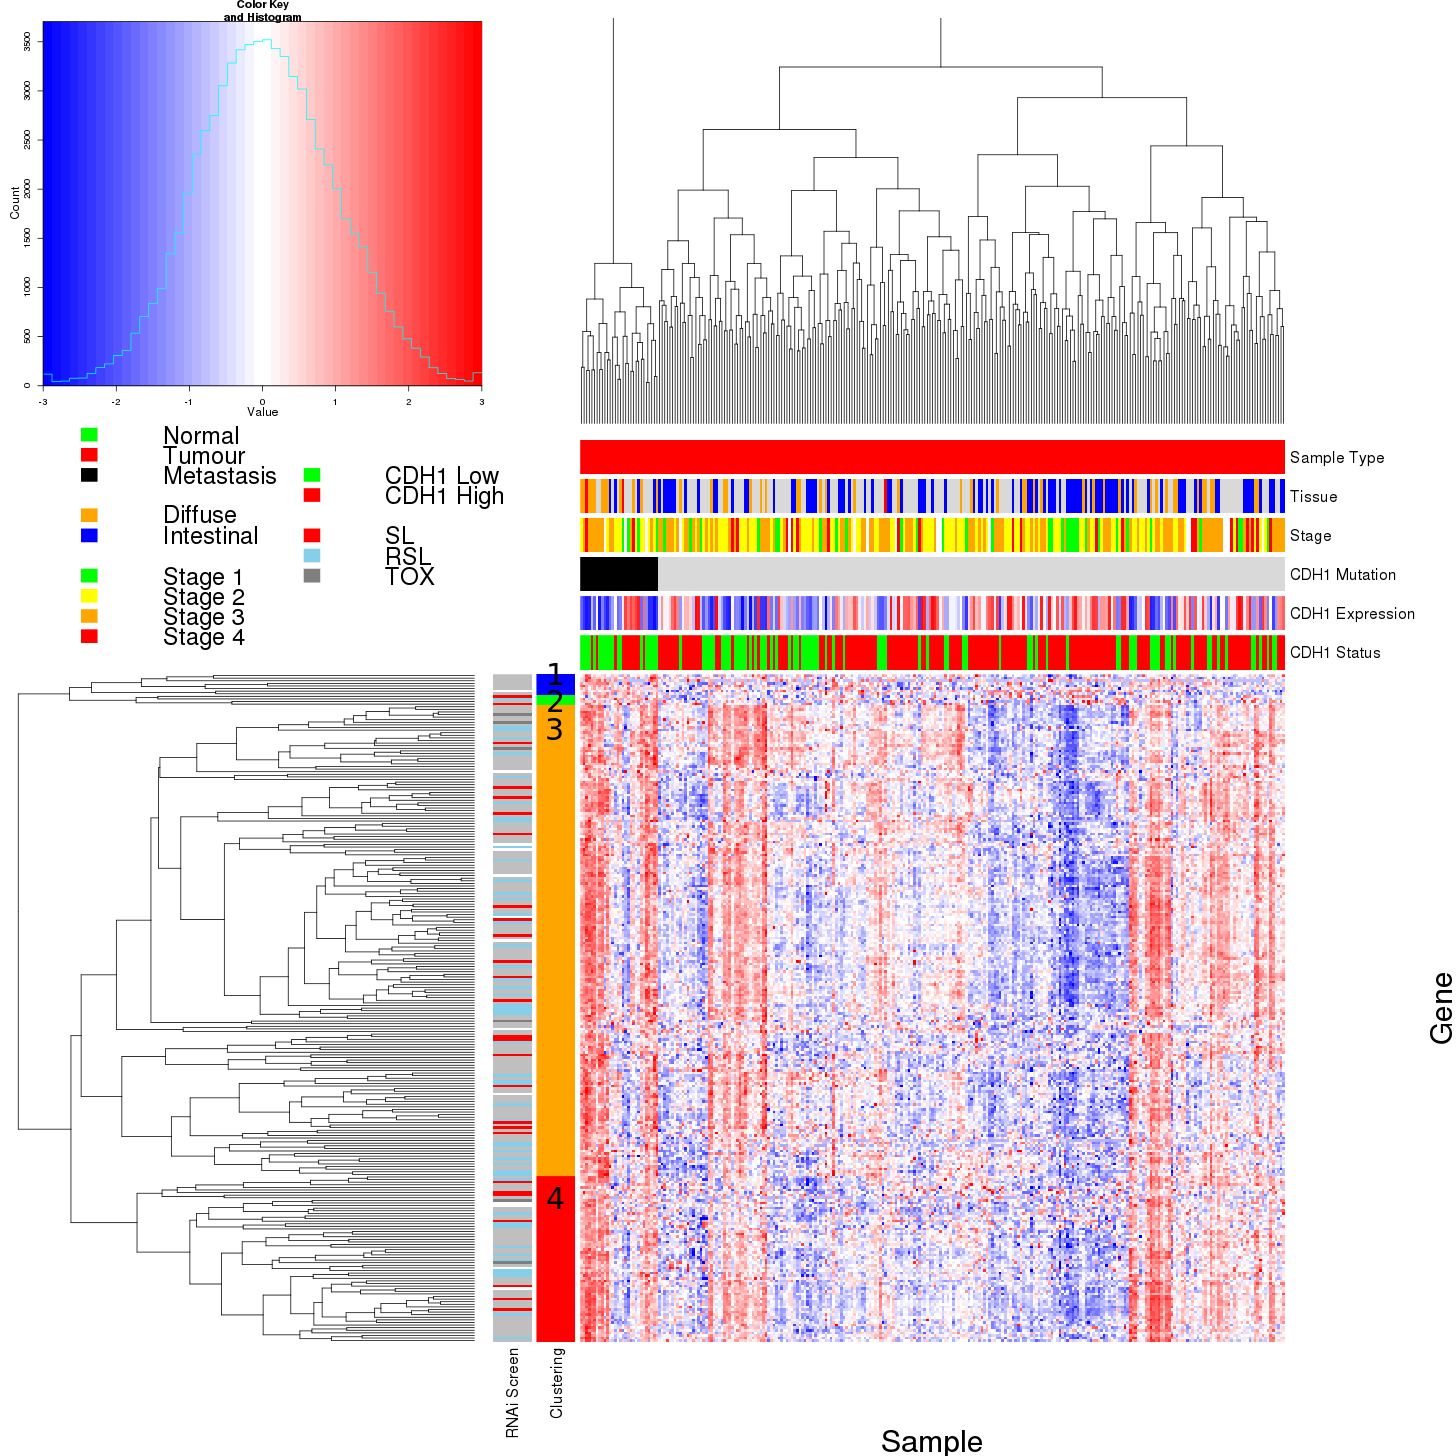
\includegraphics{CDH1_Heatmaps_Genes_Split_By_CDH1_z-trans_mtSL_cordistx_Pub_stad.png}
   }
    \caption[Synthetic lethal expression profiles of stomach samples]{\small \textbf{Synthetic lethal expression profiles of analysed samples.} Gene expression profile heatmap (correlation distance) of all samples (separated by the $\sfrac{1}{3}$ quantile of \textit{CDH1} expression) analysed in TCGA breast cancer dataset for gene expression of 4,629 candidate partners of E-cadherin (\textit{CDH1}) from SLIPT prediction (with significant FDR adjusted $p < 0.05$). Deeply clustered, inter-correlated genes form several main groups, each containing genes that were SL candidates or toxic in an siRNA screen \cite{Telford2015}. Clusters had different sample groups highly expressing the synthetic lethal candidates in \textit{CDH1} low samples, notably diffuse and \textit{CDH1} mutant samples have elevated expression in one or more distinct clusters, although there was less complexity and variation among candidate synthetic lethal partners than in breast data. \textit{CDH1} low samples also contained most of samples with \textit{CDH1} mutations.
   %This suggests that multiple targets may be needed to target \textit{CDH1} deficiency across genetic backgrounds and that combination therapy may be more effective. 
}
\label{fig:slipt_expr_stad_mtSL}
\end{mdframed}
\end{figure*}


\begin{table*}[!Hp]
\caption{Pathway composition for clusters of \textit{CDH1} partners in stomach mtSLIPT}
\label{tab:pathway_clusters_stad_mtSL}
\centering
%\begin{tiny}
%\makebox[\textwidth][c]{
\resizebox{0.666 \textwidth}{!}{
\begin{tabular}{lccc}
%\caption{Pathway composition for clusters of \textit{CDH1} partners from SLIPT}
%\label{tab:pathway_clusters}
  \large{\textbf{Pathways Over-represented in Cluster 1}} & \large{\textbf{Pathway Size}} & \large{\textbf{Cluster Genes}} & \large{\textbf{p-value (FDR)}} \\ %(833 genes)  
  \hline
  \rowcolor{Cluster_Blue!20}
  CD28 dependent PI3K/Akt signaling &  15 &   1 &   1 \\ 
  \rowcolor{Cluster_Blue!15}
  Hormone-sensitive lipase (HSL)-mediated triacylglycerol hydrolysis &  19 &   1 &   1 \\ 
  \rowcolor{Cluster_Blue!20}
  CD28 co-stimulation &  26 &   1 &   1 \\ 
  \rowcolor{Cluster_Blue!15}
  Lipid digestion, mobilization, and transport &  48 &   1 &   1 \\ 
  \rowcolor{Cluster_Blue!20}
  Costimulation by the CD28 family &  51 &   1 &   1 \\ 
  \rowcolor{Cluster_Blue!15}
  Dectin-1 mediated noncanonical NF-kB signaling &  58 &   1 &   1 \\ 
  \rowcolor{Cluster_Blue!20}
  CLEC7A (Dectin-1) signaling &  99 &   1 &   1 \\ 
  \rowcolor{Cluster_Blue!15}
  C-type lectin receptors (CLRs) & 123 &   1 &   1 \\ 
  \rowcolor{Cluster_Blue!20}
  Adaptive Immune System & 418 &   1 &   1 \\ 
  \rowcolor{Cluster_Blue!15}
  Metabolism of lipids and lipoproteins & 494 &   1 &   1 \\ 
  \rowcolor{Cluster_Blue!20}
  Interleukin-6 signaling &  10 &   0 &   1 \\ 
  \rowcolor{Cluster_Blue!15}
  Apoptosis & 150 &   0 &   1 \\ 
  \rowcolor{Cluster_Blue!20}
  Hemostasis & 445 &   0 &   1 \\ 
  \rowcolor{Cluster_Blue!15}
  Intrinsic Pathway for Apoptosis &  36 &   0 &   1 \\ 
  \rowcolor{Cluster_Blue!20}
  Cleavage of Growing Transcript in the Termination Region &  33 &   0 &   1 \\ 
  \rowcolor{Cluster_Blue!15}
  PKB-mediated events &  28 &   0 &   1 \\ 
  \rowcolor{Cluster_Blue!20}
  PI3K Cascade &  68 &   0 &   1 \\ 
  \rowcolor{Cluster_Blue!15}
  RAF/MAP kinase cascade &  10 &   0 &   1 \\ 
  \rowcolor{Cluster_Blue!20}
  Global Genomic NER (GG-NER) &  35 &   0 &   1 \\ 
  \rowcolor{Cluster_Blue!15}
  Repair synthesis for gap-filling by DNA polymerase in TC-NER &  15 &   0 &   1 \\ 
  \hline
  \\
  \cellcolor{white} \large{\textbf{Pathways Over-represented in Cluster 2}} & \large{\textbf{Pathway Size}} & \large{\textbf{Cluster Genes}} & \large{\textbf{p-value (FDR)}} \\ %(833 genes)  
  \hline
  \rowcolor{Cluster_Green!30}
  Kinesins &  22 &   1 &   1 \\ 
  \rowcolor{Cluster_Green!20}
  O-linked glycosylation of mucins &  49 &   1 &   1 \\ 
  \rowcolor{Cluster_Green!30}
  O-linked glycosylation &  59 &   1 &   1 \\ 
  \rowcolor{Cluster_Green!20}
  MHC class II antigen presentation &  85 &   1 &   1 \\ 
  \rowcolor{Cluster_Green!30}
  Factors involved in megakaryocyte development and platelet production \textcolor{Cluster_Green!30} {cellll} & 120 &   1 &   1 \\
  \rowcolor{Cluster_Green!20}
  Post-translational protein modification & 303 &   1 &   1 \\ 
  \rowcolor{Cluster_Green!30}
  Adaptive Immune System & 418 &   1 &   1 \\ 
  \rowcolor{Cluster_Green!20}
  Hemostasis & 445 &   1 &   1 \\ 
  \rowcolor{Cluster_Green!30}
  Interleukin-6 signaling &  10 &   0 &   1 \\ 
  \rowcolor{Cluster_Green!20}
  Apoptosis & 150 &   0 &   1 \\ 
  \rowcolor{Cluster_Green!30}
  Intrinsic Pathway for Apoptosis &  36 &   0 &   1 \\ 
  \rowcolor{Cluster_Green!20}
  Cleavage of Growing Transcript in the Termination Region &  33 &   0 &   1 \\ 
  \rowcolor{Cluster_Green!30}
  PKB-mediated events &  28 &   0 &   1 \\ 
  \rowcolor{Cluster_Green!20}
  PI3K Cascade &  68 &   0 &   1 \\ 
  \rowcolor{Cluster_Green!30}
  RAF/MAP kinase cascade &  10 &   0 &   1 \\ 
  \rowcolor{Cluster_Green!20}
  Global Genomic NER (GG-NER) &  35 &   0 &   1 \\ 
  \rowcolor{Cluster_Green!30}
  Repair synthesis for gap-filling by DNA polymerase in TC-NER &  15 &   0 &   1 \\ 
  \rowcolor{Cluster_Green!20}
  Gap-filling DNA repair synthesis and ligation in TC-NER &  17 &   0 &   1 \\ 
  \rowcolor{Cluster_Green!30}
  Formation of transcription-coupled NER (TC-NER) repair complex &  29 &   0 &   1 \\ 
  \rowcolor{Cluster_Green!20}
  Dual incision reaction in TC-NER &  29 &   0 &   1 \\ 
  \hline
  \\ 
  \cellcolor{white} \large{\textbf{Pathways Over-represented in Cluster 3}} & \large{\textbf{Pathway Size}} & \large{\textbf{Cluster Genes}} & \large{\textbf{p-value (FDR)}} \\ %(833 genes)  
  \hline 
  \rowcolor{Cluster_Orange!20}
  Extracellular matrix organization & 241 &  20 & $9.6 \times 10^{-9}$ \\ 
  \rowcolor{Cluster_Orange!15}
  Elastic fibre formation &  38 &   6 & $3.7 \times 10^{-8}$ \\ 
  \rowcolor{Cluster_Orange!20}
  Diseases associated with glycosaminoglycan metabolism &  26 &   5 & $3.7 \times 10^{-8}$ \\ 
  \rowcolor{Cluster_Orange!15}
  Diseases of glycosylation &  26 &   5 & $3.7 \times 10^{-8}$ \\ 
  \rowcolor{Cluster_Orange!20}
  Molecules associated with elastic fibres &  34 &   4 & $4.8 \times 10^{-5}$ \\ 
  \rowcolor{Cluster_Orange!15}
  Initial triggering of complement &  17 &   3 & $4.8 \times 10^{-5}$ \\ 
  \rowcolor{Cluster_Orange!20}
  %\begin{tabular}[c]{@{}l@{}}Regulation of Insulin-like Growth Factor (IGF) transport and \\ uptake by Insulin-like Growth Factor Binding Proteins (IGFBPs)\end{tabular} &  17 &   3 & $4.8 \times 10^{-5}$ \\
  \begin{tabular}[c]{@{}l@{}}Regulation of  IGF transport and uptake by IGFBPs\end{tabular} &  17 &   3 & $4.8 \times 10^{-5}$ \\ 
  \rowcolor{Cluster_Orange!15}
  Collagen degradation &  58 &   5 & $6.7 \times 10^{-5}$ \\ 
  \rowcolor{Cluster_Orange!20}
  Defective B4GALT7 causes EDS, progeroid type &  19 &   3 & $6.7 \times 10^{-5}$ \\ 
  \rowcolor{Cluster_Orange!15}
  Defective B3GAT3 causes JDSSDHD &  19 &   3 & $6.7 \times 10^{-5}$ \\ 
  \rowcolor{Cluster_Orange!20}
  Degradation of the extracellular matrix & 104 &   7 & $9.5 \times 10^{-5}$ \\ 
  \rowcolor{Cluster_Orange!15}
  ECM proteoglycans &  66 &   5 & 0.0002 \\ 
  \rowcolor{Cluster_Orange!20}
  A tetrasaccharide linker sequence is required for GAG synthesis &  25 & 5 3 & 0.00029 \\ 
  \rowcolor{Cluster_Orange!15}
  Non-integrin membrane-ECM interactions &  53 &   4 & 0.00079 \\ 
  \rowcolor{Cluster_Orange!20}
  Creation of C4 and C2 activators &  11 &   2 & 0.00093 \\ 
  \rowcolor{Cluster_Orange!15}
  Dermatan sulfate biosynthesis &  11 &   2 & 0.00093 \\ 
  \rowcolor{Cluster_Orange!20}
  Integrin cell surface interactions &  82 &   5 & 0.0012 \\ 
  \rowcolor{Cluster_Orange!15}
  Keratan sulfate degradation &  12 &   2 & 0.0012 \\ 
  \rowcolor{Cluster_Orange!20}
  Complement cascade &  34 &   3 & 0.0013 \\ 
  \rowcolor{Cluster_Orange!15}
  CS/DS degradation &  13 &   2 & 0.0015 \\ 
  \hline
  \\ 
  \cellcolor{white} \large{\textbf{Pathways Over-represented in Cluster 4}} & \large{\textbf{Pathway Size}} & \large{\textbf{Cluster Genes}} & \large{\textbf{p-value (FDR)}} \\ %(833 genes)  
  \hline
  \rowcolor{Cluster_Red!20}
  cGMP effects &  18 &   2 & 0.11 \\ 
  \rowcolor{Cluster_Red!15}
  Nitric oxide stimulates guanylate cyclase &  24 &   2 & 0.19 \\ 
  \rowcolor{Cluster_Red!20}
  Neurotoxicity of clostridium toxins &  10 &   1 &   1 \\ 
  \rowcolor{Cluster_Red!15}
  Platelet homeostasis &  54 &   2 &   1 \\ 
  \rowcolor{Cluster_Red!20}
  Eicosanoid ligand-binding receptors &  14 &   1 &   1 \\ 
  \rowcolor{Cluster_Red!15}
  Prolactin receptor signaling &  15 &   1 &   1 \\ 
  \rowcolor{Cluster_Red!20}
  Acyl chain remodelling of PI &  15 &   1 &   1 \\ 
  \rowcolor{Cluster_Red!15}
  Signaling by FGFR1 fusion mutants &  15 &   1 &   1 \\ 
  \rowcolor{Cluster_Red!20}
  PKA activation &  16 &   1 &   1 \\ 
  \rowcolor{Cluster_Red!15}
  PKA-mediated phosphorylation of CREB &  17 &   1 &   1 \\ 
  \rowcolor{Cluster_Red!20}
  Synthesis of glycosylphosphatidylinositol (GPI) &  17 &   1 &   1 \\ 
  \rowcolor{Cluster_Red!15}
  PKA activation in glucagon signalling &  17 &   1 &   1 \\ 
  \rowcolor{Cluster_Red!20}
  Butyrate Response Factor 1 (BRF1) destabilizes mRNA &  17 &   1 &   1 \\ 
  \rowcolor{Cluster_Red!15}
  Other semaphorin interactions &  19 &   1 &   1 \\ 
  \rowcolor{Cluster_Red!20}
  Acyl chain remodelling of PE &  21 &   1 &   1 \\ 
  \rowcolor{Cluster_Red!15}
  Signaling by Leptin &  21 &   1 &   1 \\ 
  \rowcolor{Cluster_Red!20}
  DARPP-32 events &  22 &   1 &   1 \\ 
  \rowcolor{Cluster_Red!15}
  Glucagon-like Peptide-1 (GLP1) regulates insulin secretion &  22 &   1 &   1 \\ 
  \rowcolor{Cluster_Red!20}
  Uptake and actions of bacterial toxins &  22 &   1 &   1 \\ 
  \rowcolor{Cluster_Red!15}
  Acyl chain remodelling of PC &  23 &   1 &   1 \\ 
  \hline
  \\
\end{tabular}
}
\end{table*}

\begin{figure}[!ht]
\begin{mdframed}
  \centering
  \resizebox{0.66 \columnwidth}{!}{
    \includegraphics{Venn_mtSL_siRNA_allgenes_reduced_Pub_stad.png}
   }
    \caption[Comparison of mtSLIPT in stomach to siRNA]{\small \textbf{Comparison of mtSLIPT in stomach to siRNA.} Testing the overlap of gene candidates for E-cadherin synthetic lethal partners between computational (SLIPT) and experimental screening (siRNA) approaches. The $\chi^2$ test suggests that the overlap is no more than would be expected by chance ($p = 0.281$). %A Venn diagram of all 16298 genes tested by both approaches.
}
\label{fig:Venn_allgenes_stad_mtSL}
\end{mdframed}
\end{figure}


\begin{table*}[!Hp]
\caption{Pathway composition for \textit{CDH1} partners from mtSLIPT and siRNA}
\label{tab:Venn_over-representation_stad_mtSL}
\centering
\resizebox{0.8 \textwidth}{!}{
\begin{tabular}{sl^c^c^c}
\rowstyle{\bfseries}
  Predicted only by SLIPT (217 genes) & Pathway Size & Genes Identified & p-value (FDR) \\ 
  \hline
  \rowcolor{Cluster_Red!20}
  Eukaryotic Translation Elongation &  87 &  57 & $2.8 \times 10^{-120}$ \\ 
  \rowcolor{Cluster_Red!15}
  Peptide chain elongation &  84 &  56 & $3.1 \times 10^{-120}$ \\ 
  \rowcolor{Cluster_Red!20}
  Eukaryotic Translation Termination &  84 &  55 & $2.8 \times 10^{-117}$ \\ 
  \rowcolor{Cluster_Red!15}
  Viral mRNA Translation &  82 &  54 & $4.1 \times 10^{-116}$ \\ 
  \rowcolor{Cluster_Red!20}
  Nonsense Mediated Decay independent of the Exon Junction Complex &  89 &  55 & $3.7 \times 10^{-113}$ \\ 
  \rowcolor{Cluster_Red!15}
  Formation of a pool of free 40S subunits &  94 &  55 & $2.8 \times 10^{-109}$ \\ 
  \rowcolor{Cluster_Red!20}
  Nonsense-Mediated Decay & 104 &  57 & $8.4 \times 10^{-108}$ \\ 
  \rowcolor{Cluster_Red!15}
  Nonsense Mediated Decay enhanced by the Exon Junction Complex & 104 &  57 & $8.4 \times 10^{-108}$ \\ 
  \rowcolor{Cluster_Red!20}
  L13a-mediated translational silencing of Ceruloplasmin expression & 104 &  56 & $3.4 \times 10^{-105}$ \\ 
  \rowcolor{Cluster_Red!15}
  3' -UTR-mediated translational regulation & 104 &  56 & $3.4 \times 10^{-105}$ \\ 
  \rowcolor{Cluster_Red!20}
  GTP hydrolysis and joining of the 60S ribosomal subunit & 105 &  56 & $1.4 \times 10^{-104}$ \\ 
  \rowcolor{Cluster_Red!15}
  Eukaryotic Translation Initiation & 112 &  56 & $2.8 \times 10^{-100}$ \\ 
  \rowcolor{Cluster_Red!20}
  Cap-dependent Translation Initiation & 112 &  56 & $2.8 \times 10^{-100}$ \\ 
  \rowcolor{Cluster_Red!15}
  SRP-dependent cotranslational protein targeting to membrane & 105 &  54 & $2.2 \times 10^{-99}$ \\ 
  \rowcolor{Cluster_Red!20}
  Influenza Viral RNA Transcription and Replication & 109 &  54 & $5.3 \times 10^{-97}$ \\ 
  \rowcolor{Cluster_Red!15}
  Influenza Life Cycle & 113 &  54 & $9.6 \times 10^{-95}$ \\ 
  \rowcolor{Cluster_Red!20}
  Influenza Infection & 118 &  55 & $1.7 \times 10^{-94}$ \\ 
  \rowcolor{Cluster_Red!15}
  Translation & 142 &  60 & $3.5 \times 10^{-94}$ \\ 
  \rowcolor{Cluster_Red!20}
  Infectious disease & 349 &  77 & $5.9 \times 10^{-62}$ \\ 
  \rowcolor{Cluster_Red!15}
  Extracellular matrix organization & 241 &  54 & $3 \times 10^{-52}$ \\ 
  \hline
  \\
  \rowstyle{\bfseries}
  Detected only by siRNA screen (2323 genes) & Pathway Size & Genes Identified & p-value (FDR) \\ 
  \hline
  \rowcolor{Cluster_Blue!20}
  Class A/1 (Rhodopsin-like receptors) & 282 &  69 & $1.9 \times 10^{-59}$ \\ 
  \rowcolor{Cluster_Blue!15}
  GPCR ligand binding & 363 &  78 & $2.7 \times 10^{-54}$ \\ 
  \rowcolor{Cluster_Blue!20}
  Peptide ligand-binding receptors & 175 &  41 & $1.5 \times 10^{-42}$ \\ 
  \rowcolor{Cluster_Blue!15}
  G$_{\alpha i}$ signalling events & 184 &  41 & $1.1 \times 10^{-40}$ \\ 
  \rowcolor{Cluster_Blue!20}
  Gastrin-CREB signalling pathway via PKC and MAPK & 180 &  37 & $1.5 \times 10^{-35}$ \\ 
  \rowcolor{Cluster_Blue!15}
  G$_{\alpha q}$ signalling events & 159 &  34 & $3.7 \times 10^{-35}$ \\ 
  \rowcolor{Cluster_Blue!20}
  DAP12 interactions & 159 &  27 & $1.1 \times 10^{-24}$ \\ 
  \rowcolor{Cluster_Blue!15}
  VEGFA-VEGFR2 Pathway &  91 &  19 & $1.0 \times 10^{-23}$ \\ 
  \rowcolor{Cluster_Blue!20}
  Downstream signal transduction & 146 &  24 & $1.9 \times 10^{-22}$ \\ 
  \rowcolor{Cluster_Blue!15}
  Signaling by VEGF &  99 &  19 & $2.6 \times 10^{-22}$ \\ 
  \rowcolor{Cluster_Blue!20}
  DAP12 signaling & 149 &  24 & $4.2 \times 10^{-22}$ \\ 
  \rowcolor{Cluster_Blue!15}
  Organelle biogenesis and maintenance & 264 &  34 & $4.3 \times 10^{-20}$ \\ 
  \rowcolor{Cluster_Blue!20}
  Downstream signaling of activated FGFR1 & 134 &  21 & $4.3 \times 10^{-20}$ \\ 
  \rowcolor{Cluster_Blue!15}
  Downstream signaling of activated FGFR2 & 134 &  21 & $4.3 \times 10^{-20}$ \\ 
  \rowcolor{Cluster_Blue!20}
  Downstream signaling of activated FGFR3 & 134 &  21 & $4.3 \times 10^{-20}$ \\ 
  \rowcolor{Cluster_Blue!15}
  Downstream signaling of activated FGFR4 & 134 &  21 & $4.3 \times 10^{-20}$ \\ 
  \rowcolor{Cluster_Blue!20}
  Signaling by ERBB2 & 146 &  22 & $5.3 \times 10^{-20}$ \\ 
  \rowcolor{Cluster_Blue!15}
  Signaling by FGFR & 146 &  22 & $5.3 \times 10^{-20}$ \\ 
  \rowcolor{Cluster_Blue!20}
  Signaling by FGFR1 & 146 &  22 & $5.3 \times 10^{-20}$ \\ 
  \rowcolor{Cluster_Blue!15}
  Signaling by FGFR2 & 146 &  22 & $5.3 \times 10^{-20}$ \\ 
  \hline
  \\
  \rowstyle{\bfseries}
  Intersection of SLIPT and siRNA screen (23 genes) & Pathway Size & Genes Identified & p-value (FDR) \\ 
  \hline
  \rowcolor{Cluster_Red!20!Cluster_Blue!20}
  HS-GAG degradation &  21 &   4 & $4.9 \times 10^{-6}$ \\ 
  \rowcolor{Cluster_Red!15!Cluster_Blue!15}
  Retinoid metabolism and transport &  39 &   5 & $4.9 \times 10^{-6}$ \\ 
  \rowcolor{Cluster_Red!20!Cluster_Blue!20}
  Platelet activation, signaling and aggregation & 186 &  13 & $4.9 \times 10^{-6}$ \\ 
  \rowcolor{Cluster_Red!15!Cluster_Blue!15}
  Signaling by NOTCH4 &  11 &   3 & $4.9 \times 10^{-6}$ \\ 
  \rowcolor{Cluster_Red!20!Cluster_Blue!20}
  G$_{\alpha s}$ signalling events & 100 &   8 & $5 \times 10^{-6}$ \\ 
  \rowcolor{Cluster_Red!15!Cluster_Blue!15}
  Defective EXT2 causes exostoses 2 &  12 &   3 & $5 \times 10^{-6}$ \\ 
  \rowcolor{Cluster_Red!20!Cluster_Blue!20}
  Defective EXT1 causes exostoses 1, TRPS2 and CHDS &  12 &   3 & $5 \times 10^{-6}$ \\ 
  \rowcolor{Cluster_Red!15!Cluster_Blue!15}
  Class A/1 (Rhodopsin-like receptors) & 289 &  18 & $2.2 \times 10^{-5}$ \\ 
  \rowcolor{Cluster_Red!20!Cluster_Blue!20}
  Signaling by PDGF & 173 &  11 & $2.9 \times 10^{-5}$ \\ 
  \rowcolor{Cluster_Red!15!Cluster_Blue!15}
  Circadian Clock &  34 &   4 & $2.9 \times 10^{-5}$ \\ 
  \rowcolor{Cluster_Red!20!Cluster_Blue!20}
  Signaling by ERBB4 & 139 &   9 & $4.3 \times 10^{-5}$ \\ 
  \rowcolor{Cluster_Red!15!Cluster_Blue!15}
  Role of LAT2/NTAL/LAB on calcium mobilization &  99 &   7 & $4.4 \times 10^{-5}$ \\ 
  \rowcolor{Cluster_Red!20!Cluster_Blue!20}
  Peptide ligand-binding receptors & 181 &  11 & $4.5 \times 10^{-5}$ \\ 
  \rowcolor{Cluster_Red!15!Cluster_Blue!15}
  Defective B4GALT7 causes EDS, progeroid type &  19 &   3 & $4.5 \times 10^{-5}$ \\ 
  \rowcolor{Cluster_Red!20!Cluster_Blue!20}
  Defective B3GAT3 causes JDSSDHD &  19 &   3 & $4.5 \times 10^{-5}$ \\ 
  \rowcolor{Cluster_Red!15!Cluster_Blue!15}
  Signaling by NOTCH &  80 &   6 & $4.5 \times 10^{-5}$ \\ 
  \rowcolor{Cluster_Red!20!Cluster_Blue!20}
  G$_{\alpha q}$ signalling events & 164 &  10 & $5.1 \times 10^{-5}$ \\ 
  \rowcolor{Cluster_Red!15!Cluster_Blue!15}
  Response to elevated platelet cytosolic Ca$^{2+}$ &  84 &   6 & $7.1 \times 10^{-5}$ \\ 
  \rowcolor{Cluster_Red!20!Cluster_Blue!20}
  Signaling by ERBB2 & 148 &  9 & $7.1 \times 10^{-5}$ \\ 
  \rowcolor{Cluster_Red!15!Cluster_Blue!15}
  Signaling by SCF-KIT & 129 &   8 & $8.3 \times 10^{-5}$ \\ 
  \hline
\end{tabular}
}
\end{table*}


\begin{table*}[!Htp]
\caption{Pathways for \textit{CDH1} partners from mtSLIPT in stomach cancer}
\label{tab:pathway_perm_stad_mtSL}}
\centering
\resizebox{0.8 \textwidth}{!}{
\begin{threeparttable}
\begin{tabular}{sl^c^c}
\rowstyle{\bfseries}
  Reactome Pathway & Over-representation & Permutation \\ 
  \hline
  \rowcolor{Cluster_Red!20} 
  Eukaryotic Translation Elongation & $2 \times 10^{-128}$ & $<8.802 \times 10^{-4}$ \\ 
  \rowcolor{Cluster_Red!15} 
  Peptide chain elongation & $2 \times 10^{-128}$ & $<8.802 \times 10^{-4}$ \\ 
  \rowcolor{Cluster_Red!20} 
  Eukaryotic Translation Termination & $2.3 \times 10^{-125}$ & $<8.802 \times 10^{-4}$ \\ 
  \rowcolor{Cluster_Red!15} 
  Viral mRNA Translation & $2.5 \times 10^{-124}$ & $<8.802 \times 10^{-4}$ \\ 
  \rowcolor{Cluster_Red!20} 
  Nonsense Mediated Decay independent of the Exon Junction Complex & $8.6 \times 10^{-124}$ & $<8.802 \times 10^{-4}$ \\ 
  \rowcolor{Cluster_Red!15} 
  Nonsense-Mediated Decay & $5.2 \times 10^{-117}$ & $<8.802 \times 10^{-4}$ \\ 
  \rowcolor{Cluster_Red!20} 
  Nonsense Mediated Decay enhanced by the Exon Junction Complex & $5.2 \times 10^{-117}$ & $<8.802 \times 10^{-4}$ \\ 
  \rowcolor{Cluster_Red!15} 
  Formation of a pool of free 40S subunits & $1.6 \times 10^{-116}$ & $<8.802 \times 10^{-4}$ \\ 
  \rowcolor{Cluster_Red!20} 
  L13a-mediated translational silencing of Ceruloplasmin expression & $1.3 \times 10^{-111}$ & $<8.802 \times 10^{-4}$ \\ 
  \rowcolor{Cluster_Red!15} 
  3' -UTR-mediated translational regulation & $1.3 \times 10^{-111}$ & $<8.802 \times 10^{-4}$ \\ 
  \rowcolor{Cluster_Red!20} 
  GTP hydrolysis and joining of the 60S ribosomal subunit & $6.2 \times 10^{-111}$ & $<8.802 \times 10^{-4}$ \\ 
  \rowcolor{Cluster_Red!15} 
  SRP-dependent cotranslational protein targeting to membrane & $2.9 \times 10^{-108}$ & $<8.802 \times 10^{-4}$ \\ 
  \rowcolor{Cluster_Red!20} 
  Eukaryotic Translation Initiation & $3 \times 10^{-106}$ & $<8.802 \times 10^{-4}$ \\ 
  \rowcolor{Cluster_Red!15} 
  Cap-dependent Translation Initiation & $3 \times 10^{-106}$ & $<8.802 \times 10^{-4}$ \\ 
  \rowcolor{Cluster_Red!20} 
  Influenza Viral RNA Transcription and Replication & $5.1 \times 10^{-103}$ & $<8.802 \times 10^{-4}$ \\ 
  \rowcolor{Cluster_Red!15} 
  Influenza Infection & $1.5 \times 10^{-102}$ & $<8.802 \times 10^{-4}$ \\ 
  \rowcolor{Cluster_Red!20} 
  Translation & $3.7 \times 10^{-101}$ & $<8.802 \times 10^{-4}$ \\ 
  \rowcolor{Cluster_Red!15} 
  Influenza Life Cycle & $1.4 \times 10^{-100}$ & $<8.802 \times 10^{-4}$ \\ 
  \rowcolor{Cluster_Red!20} 
  GPCR downstream signaling & $1 \times 10^{-80}$ & $0.034498$ \\ 
  \rowcolor{Cluster_Red!15} 
  Hemostasis & $1.4 \times 10^{-78}$ & $0.086519$ \\ 
  \rowcolor{Cluster_Red!20} 
  Extracellular matrix organization & $1.5 \times 10^{-67}$ & $0.040016$ \\ 
  \rowcolor{Cluster_Red!15} 
  Developmental Biology & $1.8 \times 10^{-66}$ & $0.18385$ \\ 
  \rowcolor{Cluster_Red!20} 
  Infectious disease & $7.3 \times 10^{-66}$ & $0.068426$ \\ 
  \rowcolor{Cluster_Red!15} 
  Signalling by NGF & $8.5 \times 10^{-63}$ & $0.16798$ \\ 
  \rowcolor{Cluster_Red!20} 
  Metabolism of lipids and lipoproteins & $4.9 \times 10^{-58}$ & $0.51411$ \\ 
  \rowcolor{Cluster_Red!15} 
  Platelet activation, signaling and aggregation & $2.7 \times 10^{-55}$ & $0.081717$ \\ 
  \rowcolor{Cluster_Red!20} 
  GPCR ligand binding & $7.3 \times 10^{-55}$ & $0.28898$ \\ 
  \rowcolor{Cluster_Red!15} 
  Signaling by PDGF & $8.4 \times 10^{-55}$ & $0.16025$ \\ 
  \rowcolor{Cluster_Red!20} 
  Class A/1 (Rhodopsin-like receptors) & $3.2 \times 10^{-54}$ & $0.22801$ \\ 
  \rowcolor{Cluster_Red!15} 
  Fc epsilon receptor (FCERI) signaling & $6.2 \times 10^{-53}$ & $0.15229$ \\ 
  \rowcolor{Cluster_Red!20} 
  Adaptive Immune System & $5.1 \times 10^{-52}$ & $0.037698$ \\ 
  \rowcolor{Cluster_Red!15} 
  Signaling by ERBB4 & $5.9 \times 10^{-52}$ & $0.10088$ \\ 
  \rowcolor{Cluster_Red!20} 
  Axon guidance & $8.8 \times 10^{-52}$ & $0.40234$ \\ 
  \rowcolor{Cluster_Red!15} 
  Formation of the ternary complex, and subsequently, the 43S complex & $1.6 \times 10^{-51}$ & $0.00088017$ \\ 
  \rowcolor{Cluster_Red!20} 
  Ribosomal scanning and start codon recognition & $2.2 \times 10^{-50}$ & $0.00088017$ \\ 
  \rowcolor{Cluster_Red!15} 
  Translation initiation complex formation & $2.2 \times 10^{-50}$ & $0.0017305$ \\ 
  \rowcolor{Cluster_Red!20} 
  NGF signalling via TRKA from the plasma membrane & $6.7 \times 10^{-50}$ & $0.28811$ \\ 
  \rowcolor{Cluster_Red!15} 
  \begin{tabular}[c]{@{}l@{}}Activation of the mRNA upon binding of the cap-binding complex and eIFs,\\and subsequent binding to 43S \end{tabular} & $7.1 \times 10^{-50}$ & $0.0017305$ \\ 
  \rowcolor{Cluster_Red!20} 
  Transmembrane transport of small molecules & $1.8 \times 10^{-49}$ & $0.081229$ \\ 
  \rowcolor{Cluster_Red!15} 
  Signaling by ERBB2 & $5.9 \times 10^{-49}$ & $0.11896$ \\ 
  \rowcolor{Cluster_Red!20} 
  Rho GTPase cycle & $3.6 \times 10^{-48}$ & $0.035735$ \\ 
  \rowcolor{Cluster_Red!15} 
  G_${\alpha s}$ signalling events & $1.1 \times 10^{-47}$ & $0.0088487$ \\ 
  \rowcolor{Cluster_Red!20} 
  Downstream signal transduction & $1.7 \times 10^{-47}$ & $0.11909$ \\ 
  \rowcolor{Cluster_Red!15} 
  Signaling by FGFR & $1.7 \times 10^{-47}$ & $0.11896$ \\ 
  \rowcolor{Cluster_Red!20} 
  Signaling by FGFR1 & $1.7 \times 10^{-47}$ & $0.11896$ \\ 
  \rowcolor{Cluster_Red!15} 
  Signaling by FGFR2 & $1.7 \times 10^{-47}$ & $0.11896$ \\ 
  \rowcolor{Cluster_Red!20} 
  Signaling by FGFR3 & $1.7 \times 10^{-47}$ & $0.11896$ \\ 
  \rowcolor{Cluster_Red!15} 
  Signaling by FGFR4 & $1.7 \times 10^{-47}$ & $0.11896$ \\ 
  \rowcolor{Cluster_Red!20} 
  DAP12 interactions & $1.9 \times 10^{-47}$ & $0.28811$ \\ 
  \rowcolor{Cluster_Red!15} 
  DAP12 signaling & $1 \times 10^{-46}$ & $0.12442$ \\ 
  \hline
\end{tabular}
\begin{tablenotes}
\raggedright \small
Over-representation (hypergeometric test) and Permutation p-values adjusted for multiple tests across pathways (FDR). Significant pathways are marked in bold (FDR $ < 0.05$) and italics (FDR $ < 0.1$).
\end{tablenotes}
\end{threeparttable}
}
\end{table*}

\begin{table*}[!Htp]
\caption{Pathways for \textit{CDH1} partners from mtSLIPT in stomach and siRNA screen}
\label{tab:pathway_perm_overlap_stad_mtSL}
\centering
\resizebox{0.8 \textwidth}{!}{
\begin{threeparttable}
\begin{tabular}{sl^c^c}
\rowstyle{\bfseries}
  Reactome Pathway & Over-representation & Permutation \\ 
  \hline
  \rowcolor{Cluster_Red!20!Cluster_Blue!20} 
  Signaling by NOTCH4 & $4.9 \times 10^{-6}$ & $0.050121$ \\ 
  \rowcolor{Cluster_Red!15!Cluster_Blue!15} 
  HS-GAG degradation & $4.9 \times 10^{-6}$ & $0.013193$ \\ 
  \rowcolor{Cluster_Red!20!Cluster_Blue!20} 
  Platelet activation, signaling and aggregation & $4.9 \times 10^{-6}$ & $0.28053$ \\ 
  \rowcolor{Cluster_Red!15!Cluster_Blue!15} 
  Retinoid metabolism and transport & $4.9 \times 10^{-6}$ & $0.0927$ \\ 
  \rowcolor{Cluster_Red!20!Cluster_Blue!20} 
  Defective EXT2 causes exostoses 2 & $5 \times 10^{-6}$ & $0.14898$ \\ 
  \rowcolor{Cluster_Red!15!Cluster_Blue!15} 
  Defective EXT1 causes exostoses 1, TRPS2 and CHDS & $5 \times 10^{-6}$ & $0.14898$ \\ 
  \rowcolor{Cluster_Red!20!Cluster_Blue!20} 
  G_${\alpha s}$ signalling events & $5 \times 10^{-6}$ & $0.048426$ \\ 
  \rowcolor{Cluster_Red!15!Cluster_Blue!15} 
  Class A/1 (Rhodopsin-like receptors) & $2.2 \times 10^{-5}$ & $0.60435$ \\ 
  \rowcolor{Cluster_Red!20!Cluster_Blue!20} 
  Signaling by PDGF & $2.9 \times 10^{-5}$ & $0.43907$ \\ 
  \rowcolor{Cluster_Red!15!Cluster_Blue!15} 
  Circadian Clock & $2.9 \times 10^{-5}$ & $0.012519$ \\ 
  \rowcolor{Cluster_Red!20!Cluster_Blue!20} 
  Signaling by ERBB4 & $4.3 \times 10^{-5}$ & $0.12835$ \\ 
  \rowcolor{Cluster_Red!15!Cluster_Blue!15} 
  Role of LAT2/NTAL/LAB on calcium mobilization & $4.4 \times 10^{-5}$ & $0.27344$ \\ 
  \rowcolor{Cluster_Red!20!Cluster_Blue!20} 
  Defective B4GALT7 causes EDS, progeroid type & $4.5 \times 10^{-5}$ & $0.23536$ \\ 
  \rowcolor{Cluster_Red!15!Cluster_Blue!15} 
  Defective B3GAT3 causes JDSSDHD & $4.5 \times 10^{-5}$ & $0.23536$ \\ 
  \rowcolor{Cluster_Red!20!Cluster_Blue!20} 
  Peptide ligand-binding receptors & $4.5 \times 10^{-5}$ & $0.41193$ \\ 
  \rowcolor{Cluster_Red!15!Cluster_Blue!15} 
  Signaling by NOTCH & $4.5 \times 10^{-5}$ & $0.10912$ \\ 
  \rowcolor{Cluster_Red!20!Cluster_Blue!20} 
  G_${\alpha q}$ signalling events & $5.1 \times 10^{-5}$ & $0.28937$ \\ 
  \rowcolor{Cluster_Red!15!Cluster_Blue!15} 
  Signaling by ERBB2 & $7.1 \times 10^{-5}$ & $0.50797$ \\ 
  \rowcolor{Cluster_Red!20!Cluster_Blue!20} 
  Response to elevated platelet cytosolic Ca$^{2+}$ & $7.1 \times 10^{-5}$ & $0.38513$ \\ 
  \rowcolor{Cluster_Red!15!Cluster_Blue!15} 
  Signaling by SCF-KIT & $8.3 \times 10^{-5}$ & $0.55412$ \\ 
  \rowcolor{Cluster_Red!20!Cluster_Blue!20} 
  PI3K events in ERBB4 signaling & $0.0001$ & $0.24486$ \\ 
  \rowcolor{Cluster_Red!15!Cluster_Blue!15} 
  PIP3 activates AKT signaling & $0.0001$ & $0.24486$ \\ 
  \rowcolor{Cluster_Red!20!Cluster_Blue!20} 
  Collagen formation & $0.0001$ & $0.15296$ \\ 
  \rowcolor{Cluster_Red!15!Cluster_Blue!15} 
  PI3K events in ERBB2 signaling & $0.0001$ & $0.24486$ \\ 
  \rowcolor{Cluster_Red!20!Cluster_Blue!20} 
  PI-3K cascade:FGFR1 & $0.0001$ & $0.24486$ \\ 
  \rowcolor{Cluster_Red!15!Cluster_Blue!15} 
  PI-3K cascade:FGFR2 & $0.0001$ & $0.24486$ \\ 
  \rowcolor{Cluster_Red!20!Cluster_Blue!20} 
  PI-3K cascade:FGFR3 & $0.0001$ & $0.24486$ \\ 
  \rowcolor{Cluster_Red!15!Cluster_Blue!15} 
  PI-3K cascade:FGFR4 & $0.0001$ & $0.24486$ \\ 
  \rowcolor{Cluster_Red!20!Cluster_Blue!20} 
  Growth hormone receptor signaling & $0.0001$ & $0.057494$ \\ 
  \rowcolor{Cluster_Red!15!Cluster_Blue!15} 
  PI3K Cascade & $0.00011$ & $0.20906$ \\ 
  \rowcolor{Cluster_Red!20!Cluster_Blue!20} 
  Effects of PIP2 hydrolysis & $0.00012$ & $0.14898$ \\ 
  \rowcolor{Cluster_Red!15!Cluster_Blue!15} 
  A tetrasaccharide linker sequence is required for GAG synthesis & $0.00012$ & $0.29766$ \\ 
  \rowcolor{Cluster_Red!20!Cluster_Blue!20} 
  PI3K/AKT activation & $0.00013$ & $0.24486$ \\ 
  \rowcolor{Cluster_Red!15!Cluster_Blue!15} 
  GAB1 signalosome & $0.00013$ & $0.4648$ \\ 
  \rowcolor{Cluster_Red!20!Cluster_Blue!20} 
  Diseases associated with glycosaminoglycan metabolism & $0.00013$ & $0.050121$ \\ 
  \rowcolor{Cluster_Red!15!Cluster_Blue!15} 
  Diseases of glycosylation & $0.00013$ & $0.050121$ \\ 
  \rowcolor{Cluster_Red!20!Cluster_Blue!20} 
  Heparan sulfate/heparin (HS-GAG) metabolism & $0.00016$ & $0.19$ \\ 
  \rowcolor{Cluster_Red!15!Cluster_Blue!15} 
  HS-GAG biosynthesis & $0.00016$ & $0.29681$ \\ 
  \rowcolor{Cluster_Red!20!Cluster_Blue!20} 
  Integrin alphaIIb beta3 signaling & $0.00016$ & $0.63007$ \\ 
  \rowcolor{Cluster_Red!15!Cluster_Blue!15} 
  Interferon gamma signaling & $0.00018$ & $0.43088$ \\ 
  \rowcolor{Cluster_Red!20!Cluster_Blue!20} 
  Gastrin-CREB signalling pathway via PKC and MAPK & $0.00018$ & $0.77958$ \\ 
  \rowcolor{Cluster_Red!15!Cluster_Blue!15} 
  Chemokine receptors bind chemokines & $0.00023$ & $0.62702$ \\ 
  \rowcolor{Cluster_Red!20!Cluster_Blue!20} 
  Downstream signal transduction & $0.00027$ & $0.54921$ \\ 
  \rowcolor{Cluster_Red!15!Cluster_Blue!15} 
  Platelet homeostasis & $0.00029$ & $0.24577$ \\ 
  \rowcolor{Cluster_Red!20!Cluster_Blue!20} 
  IRS-mediated signalling & $0.00029$ & $0.31766$ \\ 
  \rowcolor{Cluster_Red!15!Cluster_Blue!15} 
  G_${\alpha i}$ signalling events & $0.00029$ & $<2.749 \times 10^{-4}$ \\ 
  \rowcolor{Cluster_Red!20!Cluster_Blue!20} 
  Diseases of signal transduction & $0.00029$ & $0.65733$ \\ 
  \rowcolor{Cluster_Red!15!Cluster_Blue!15} 
  Signaling by activated point mutants of FGFR1 & $0.00029$ & $0.24892$ \\ 
  \rowcolor{Cluster_Red!20!Cluster_Blue!20} 
  FGFR1c ligand binding and activation & $0.00029$ & $0.24892$ \\ 
  \rowcolor{Cluster_Red!15!Cluster_Blue!15} 
  Signaling by NOTCH3 & $0.00029$ & $0.017419$ \\ 
  \hline
\end{tabular}
\begin{tablenotes}
\raggedright \small
Over-representation (hypergeometric test) and Permutation p-values adjusted for multiple tests across pathways (FDR). Significant pathways are marked in bold (FDR $ < 0.05$) and italics (FDR $ < 0.1$).
\end{tablenotes}
\end{threeparttable}
}
\end{table*}  

\begin{table*}[!ht]
\caption{Candidate synthetic lethal metagenes against \textit{CDH1} from mtSLIPT in stomach cancer}
\label{tab:metagene_stad_mtSL}
\centering
\resizebox{1 \textwidth}{!}{
\begin{threeparttable}
\begin{tabular}{sl^l^c^c^c^c^c}
\rowstyle{\bfseries}
 Pathway & ID & Observed & Expected & $\chi^2$value & p-value & p-value (FDR) \\
  \hline
  \rowcolor{black!10}
  Prostacyclin signalling through prostacyclin receptor & 392851 & 1 & 10.07 & 26.53 & $1.7307 \times 10^{-6}$ & $0.0028590$\\
  \rowcolor{black!5}
  Cell surface interactions at the vascular wall & 202733 & 3 & 10.07 & 21.11 & $2.6107 \times 10^{-5}$ & $0.00642330$\\
  \rowcolor{black!10}
  The NLRP1 inflammasome & 844455 & 3 & 10.07 & 21.11 & $2.6107 \times 10^{-5}$ & $0.00642330$\\
  \rowcolor{black!5}
  Innate Immune System & 168249 & 6 & 10.07 & 21.07 & $2.6548 \times 10^{-5}$ & $0.00642330$\\
  \rowcolor{black!10}
  Keratan sulfate\/keratin metabolism & 1638074 & 4 & 10.07 & 20.65 & $3.2861 \times 10^{-5}$ & $0.00642330$\\
  \rowcolor{black!5}
  Keratan sulfate biosynthesis & 2022854 & 4 & 10.07 & 20.65 & $3.2861 \times 10^{-5}$ & $0.00642330$\\
  \rowcolor{black!10}
  Signaling by SCF-KIT & 1433557 & 5 & 10.07 & 20.64 & $3.3045 \times 10^{-5}$ & $0.00642330$\\
  \rowcolor{black!5}
  VEGFA-VEGFR2 Pathway & 4420097 & 5 & 10.07 & 20.64 & $3.3045 \times 10^{-5}$ & $0.00642330$\\
  \rowcolor{black!10}
  ERK1 activation & 110056 & 21 & 10.07 & 20.12 & $4.277 \times 10^{-5}$ & $0.00642330$\\
  \rowcolor{black!5}
  Cholesterol biosynthesis & 191273 & 21 & 10.07 & 20.12 & $4.277 \times 10^{-5}$ & $0.00642330$\\
  \rowcolor{black!10}
  G2 Phase & 68911 & 21 & 10.07 & 20.12 & $4.277 \times 10^{-5}$ & $0.00642330$\\
  \rowcolor{black!5}
  p130Cas linkage to MAPK signaling for integrins & 372708 & 2 & 10.07 & 19.08 & $7.1872 \times 10^{-5}$ & $0.00651340$\\
  \rowcolor{black!10}
  cGMP effects & 418457 & 8 & 10.07 & 19.01 & $7.4597 \times 10^{-5}$ & $0.00651340$\\
  \rowcolor{black!5}
   \begin{tabular}[c]{@{}l@{}}Regulation of cytoskeletal remodeling and cell spreading by IPP \\ complex components \end{tabular} & 446388 & 8 & 10.07 & 19.01 & $7.4597 \times 10^{-5}$ & $0.00651340$\\
  \rowcolor{black!10}
  Post-translational modification: synthesis of GPI-anchored proteins & 163125 & 20 & 10.07 & 18.59 & $9.1878 \times 10^{-5}$ & $0.00651340$\\
  \rowcolor{black!5}
  Fcgamma receptor (FCGR) dependent phagocytosis & 2029480 & 3 & 10.07 & 17.95 & $0.00012676$ & $0.00651340$\\
  \rowcolor{black!10}
  A third proteolytic cleavage releases NICD & 157212 & 7 & 10.07 & 17.90 & $0.00012995$ & $0.00651340$\\
  \rowcolor{black!5}
  Signalling by NGF & 166520 & 7 & 10.07 & 17.90 & $0.00012995$ & $0.00651340$\\
  \rowcolor{black!10}
  Signaling by VEGF & 194138 & 7 & 10.07 & 17.90 & $0.00012995$ & $0.00651340$\\
  \rowcolor{black!5}
  Regulation of thyroid hormone activity & 350864 & 7 & 10.07 & 17.90 & $0.00012995$ & $0.00651340$\\
  \rowcolor{black!10}
  Nitric oxide stimulates guanylate cyclase & 392154 & 7 & 10.07 & 17.90 & $0.00012995$ & $0.00651340$\\
  \rowcolor{black!5}
  Platelet homeostasis & 418346 & 7 & 10.07 & 17.90 & $0.00012995$ & $0.00651340$\\
  \rowcolor{black!10}
  Termination of translesion DNA synthesis & 5656169 & 20 & 10.07 & 17.46 & $0.00016155$ & $0.00651340$\\
  \rowcolor{black!5}
  PI3K events in ERBB4 signaling & 1250342 & 4 & 10.07 & 17.26 & $0.00017862$ & $0.00651340$\\
  \rowcolor{black!5}
  PIP3 activates AKT signaling & 1257604 & 4 & 10.07 & 17.26 & $0.00017862$ & $0.00651340$\\
   \hline
\end{tabular}
\begin{tablenotes}
\raggedright \small
Strongest candidate SL partners for \textit{CDH1} by mtSLIPT with observed and expected mutant samples with low expression of partner metagenes
\end{tablenotes}
\end{threeparttable}
}
\end{table*}


